\documentclass[11pt, a4paper]{article}
\usepackage{natbib}         % Pour la bibliographie
\usepackage{graphicx}        
\usepackage[T1]{fontenc}    % Encodage des accents
\usepackage[utf8]{inputenc} % Lui aussi
\usepackage[french]{babel} % Pour la traduction française
\usepackage{numprint}       % Histoire que les chiffres soient bien
\usepackage{amsmath}        % La base pour les maths
\usepackage{cases}
\usepackage{mathrsfs}       % Quelques symboles supplémentaires
\usepackage{stmaryrd}
\usepackage{amssymb}        % encore des symboles.
\usepackage{amsfonts}       % Des fontes, eg pour \mathbb.
\usepackage{mathtools}
\usepackage[svgnames]{xcolor} % De la couleur
\usepackage{geometry}       % Gérer correctement la taille
\title{Etude stabilité numérique}
\author{paul.beguin }
\date{May 2020}
\begin{document}
\maketitle
\section{Manifestation d'instabilité du schéma}
Cette étude fut modifiée par le glissement trop élevé des blocs du glacier en l'absence de perturbation extérieur. La question étant de comprendre l'origine de ce glissement et pouvoir adapter le modèle. Dans cette partie, nous nous intéresserons aux résultats initiaux et au comportement du système sans préoccupations particulières pour le glissement. Les paramètres numériques retenues dans cette partie sont présentés tableau . La valeur de $\delta t$ respecte le critère de stabilité imposée par l'élasticité des liaisons entre les blocs.
\begin{table}[h!]
    \centering
    \begin{tabular}{|ccc|}
         \hline
         \textbf{Paramètres} & \textbf{Valeurs} & \textbf{Unités} \\
         \hline
         $T_{tot}$ & 300 & s \\
         \hline
         $L_{tot}$ & 40 & km \\
         \hline
         $\delta t$ & 0.012 & s \\
         \hline
         $\delta l$ & 800 & m \\
         \hline
         $N_{t}$ & 2500 & - \\
         \hline
         $N_{p}$ & 50 & - \\
         \hline 
    \end{tabular}
    \caption{Paramètres spatial et temporel de discrétisation pour schéma instable}
    \label{PaSimuInsta}
\end{table}
\setlength{\parindent}{1cm} La figure  présente les déplacements totaux et perturbés à certains blocs du glacier. La figure de droite affiche les déplacements perturbés (auxquels sont soustraits les déplacements de glissement d'équilibre) sans force de perturbation. Les vitesses d'équilibre semblent être donc trop faibles.
\begin{figure}[h!]
    \centering
    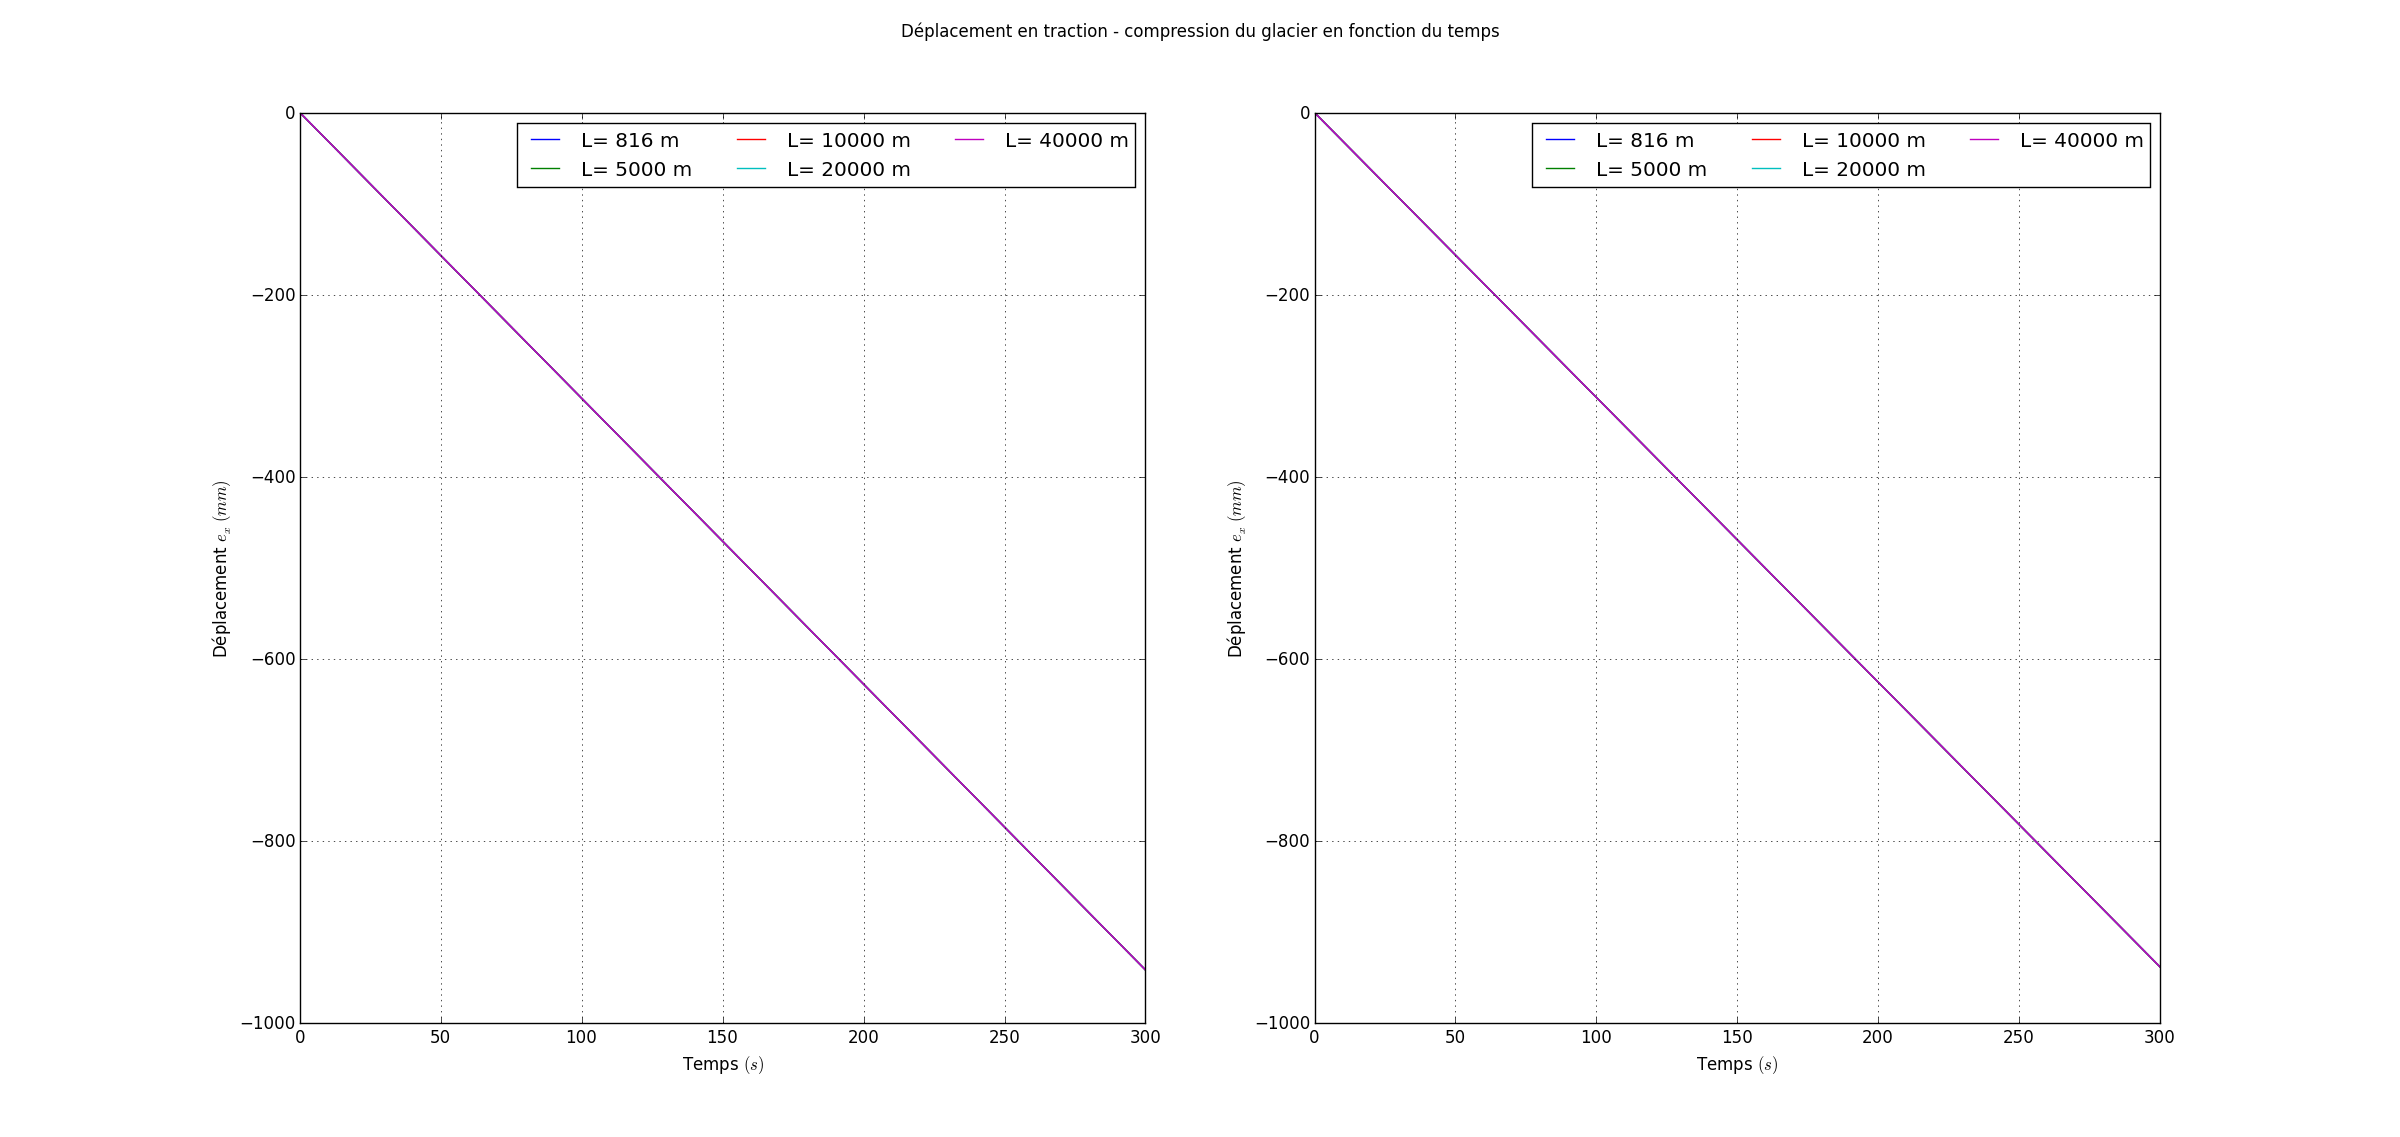
\includegraphics[width=1\linewidth]{figures/Part1/DeplacementDt0012Init.png}
    \caption{Déplacements modèle instable au cours du temps sans force de perturbation}
    \label{UtInstable}
\end{figure}
\\

La figure \ref{UtdInstable} montre un caractère oscillant du système. Ces figures sont dominées par l'affichage de la vitesse au dernier bloc, car étant la dernière courbe affichée et car subissant des oscillations très courtes. Toutefois le système ne prend pas encore en compte de force de perturbation. D'autre part les glissements initiaux des blocs entre eux (considérés à l'équilibre) étant nuls avec la loi de Weertman, aucunes forces élastiques de liaisons ne devraient apparaître entre ceux-ci. Les oscillations des vitesses glissements ne semblent pas justifiées.
\\

\begin{figure}[h!]
    \centering
    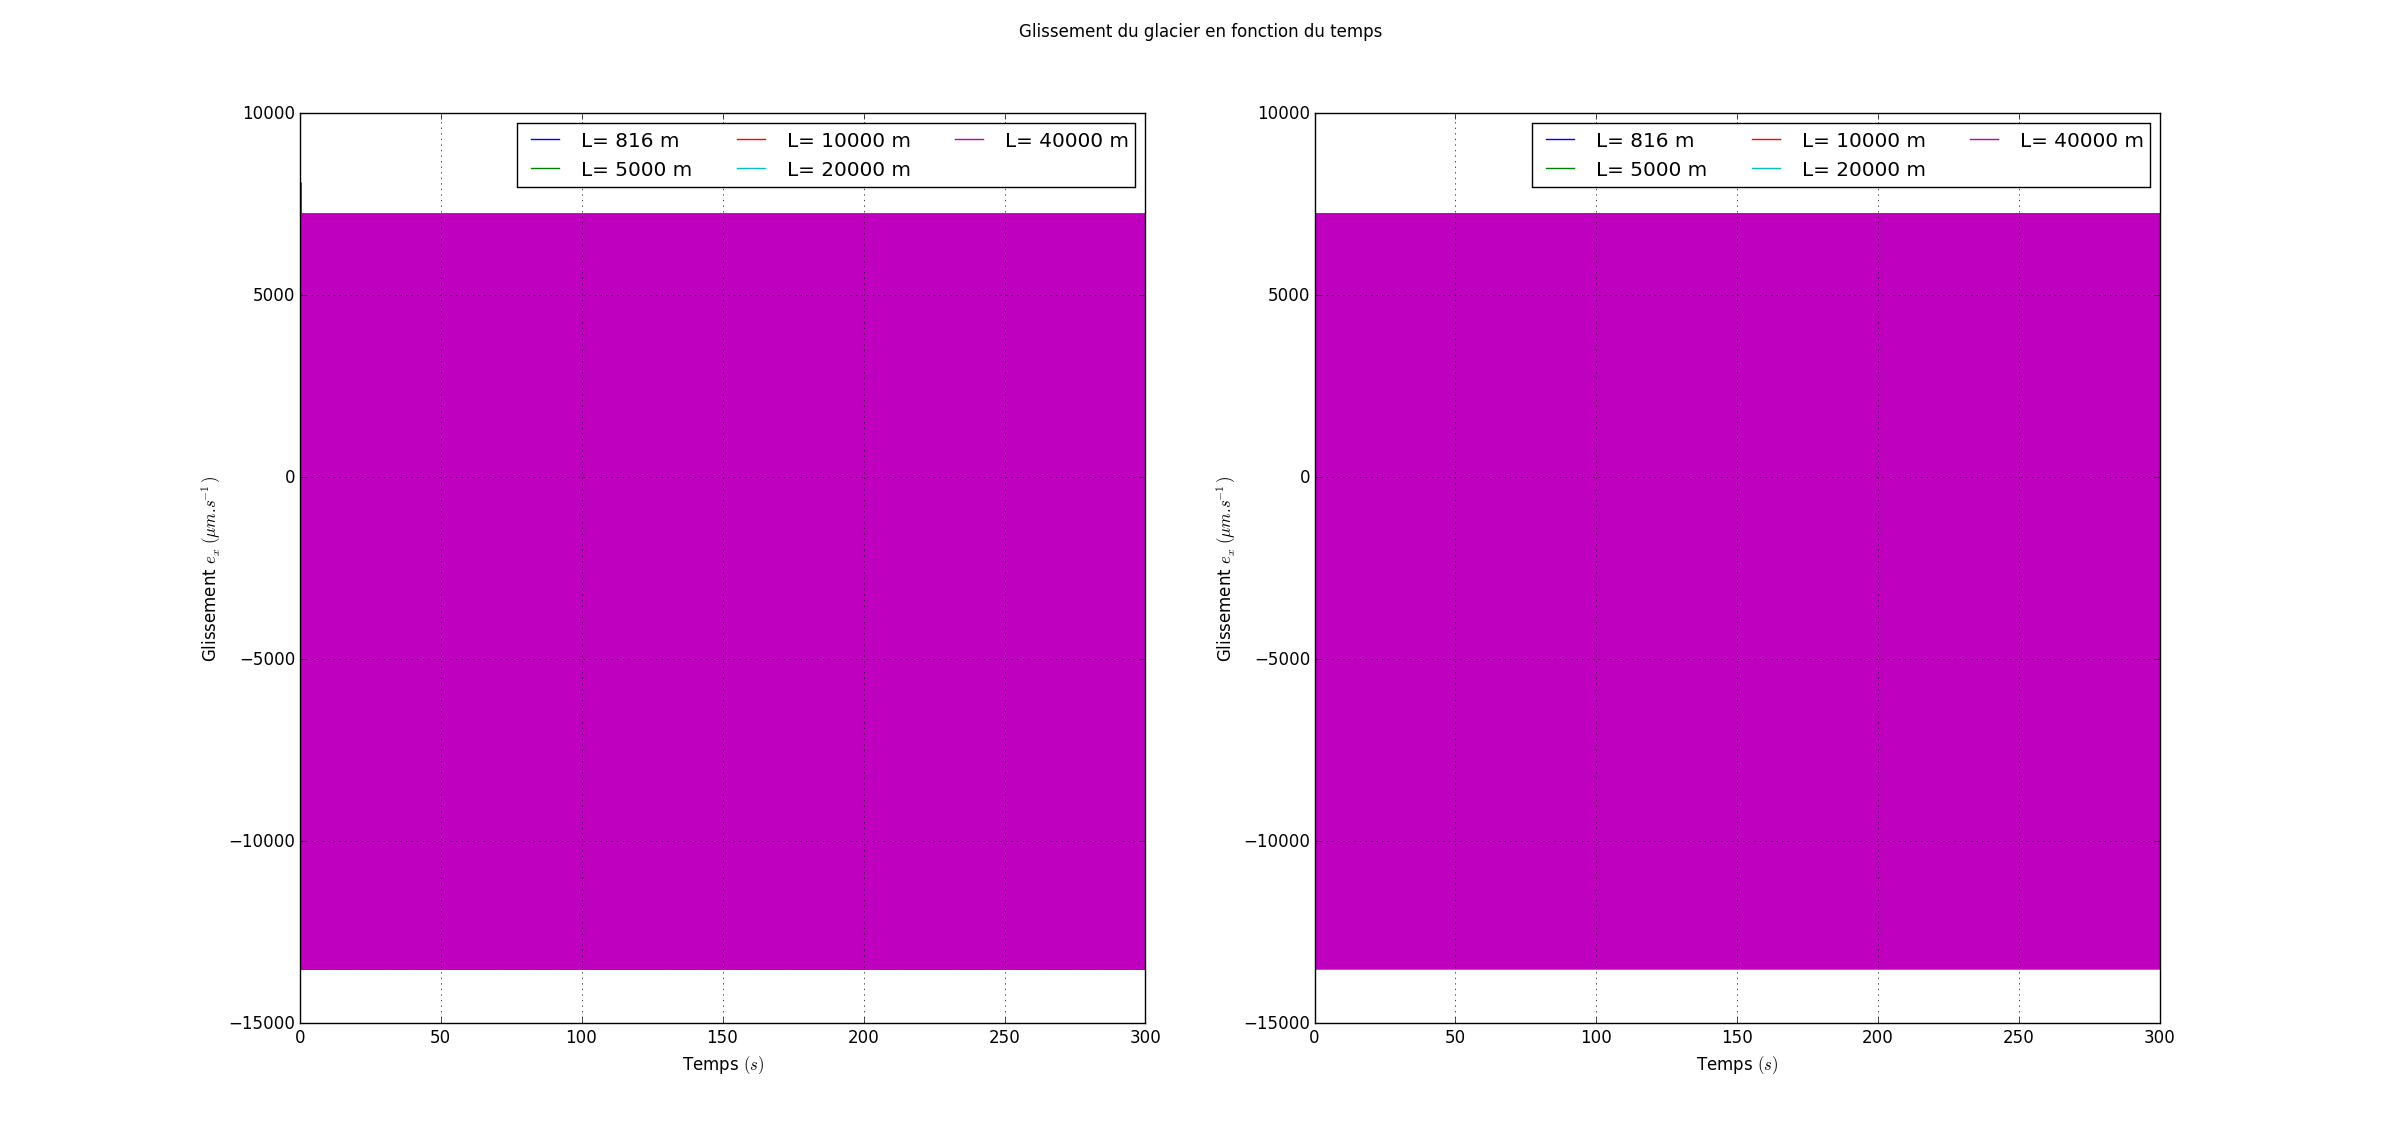
\includegraphics[width=1\linewidth]{figures/Part1/VitesseDt0012.png}
    \caption{Vitesses de glissement instable au cours du temps sans force de perturbation}
    \label{UtdInstable}
\end{figure}
On peut remarquer également qu'en changeant le pas de temps $\delta t$ à $0.001s$, on se place dans un autre régime de stabilité pour la vitesse. La figure \ref{UtdInstable2} présente le système non oscillant, mais avec toujours une vitesse pour les blocs toujours trop importante. Le système semble atteindre une autre vitesse d'équilibre. La figure \ref{UtInstable2} présente le déplacement du système encore pour $\delta t = 0.001s$. Le pas de temps est donc plus de 10fois plus faible que pour les résultats figures \ref{UtInstable} et \ref{UtdInstable}. Le système ne semble toujours pas stable.
\\

\begin{figure}[h!]
	\centering
	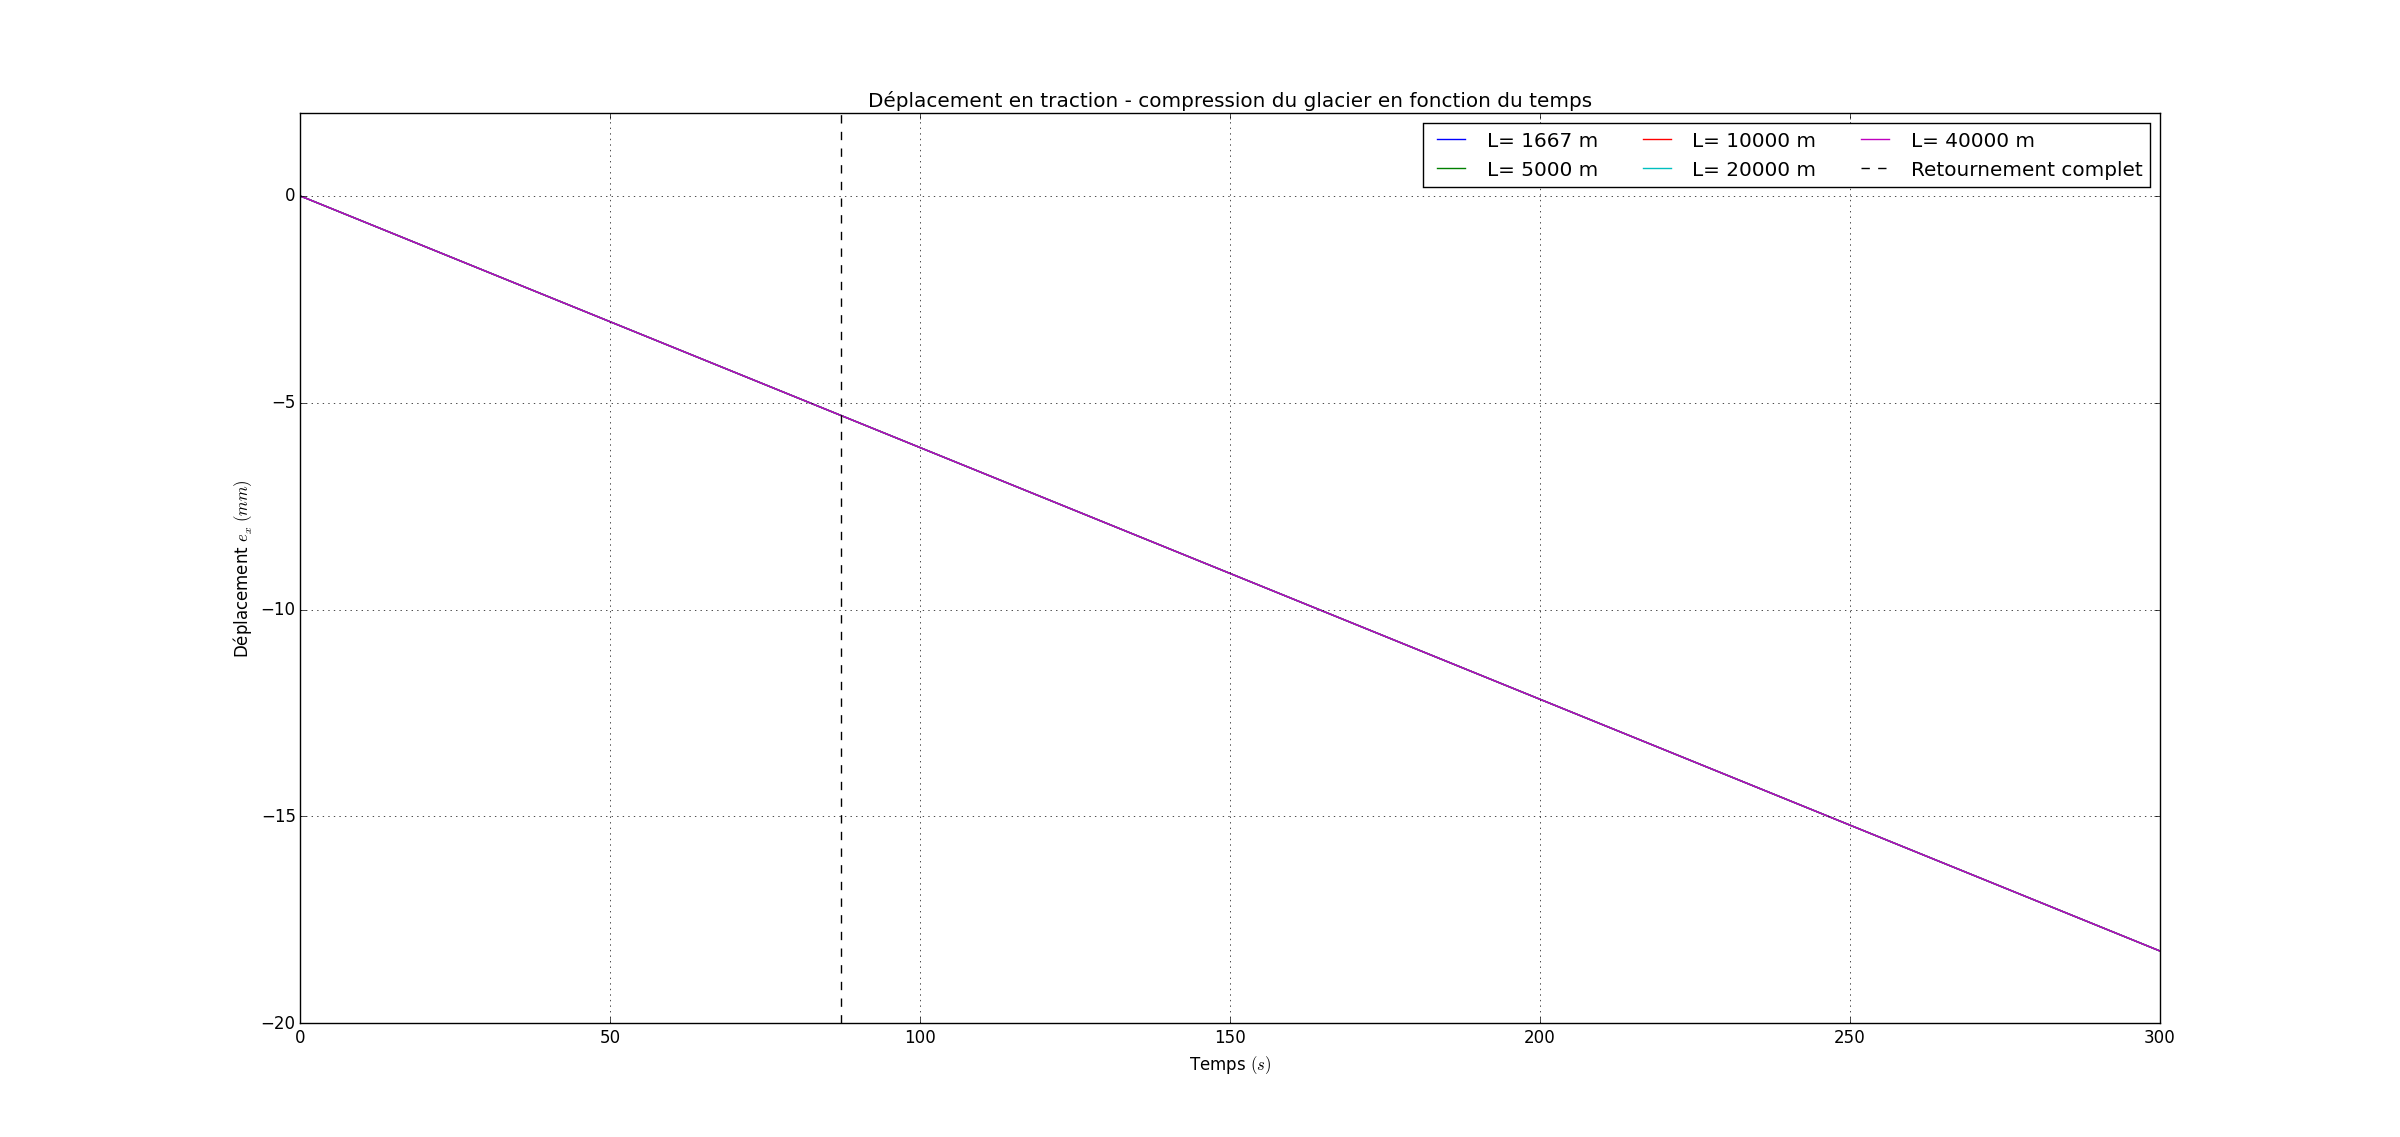
\includegraphics[width=1\linewidth]{figures/Part1/DeplacementDt0001.png}
	\caption{Déplacement pour $\delta t= 0.001s$}
	\label{UtInstable2}
\end{figure}
\begin{figure}[h!]
	\centering
	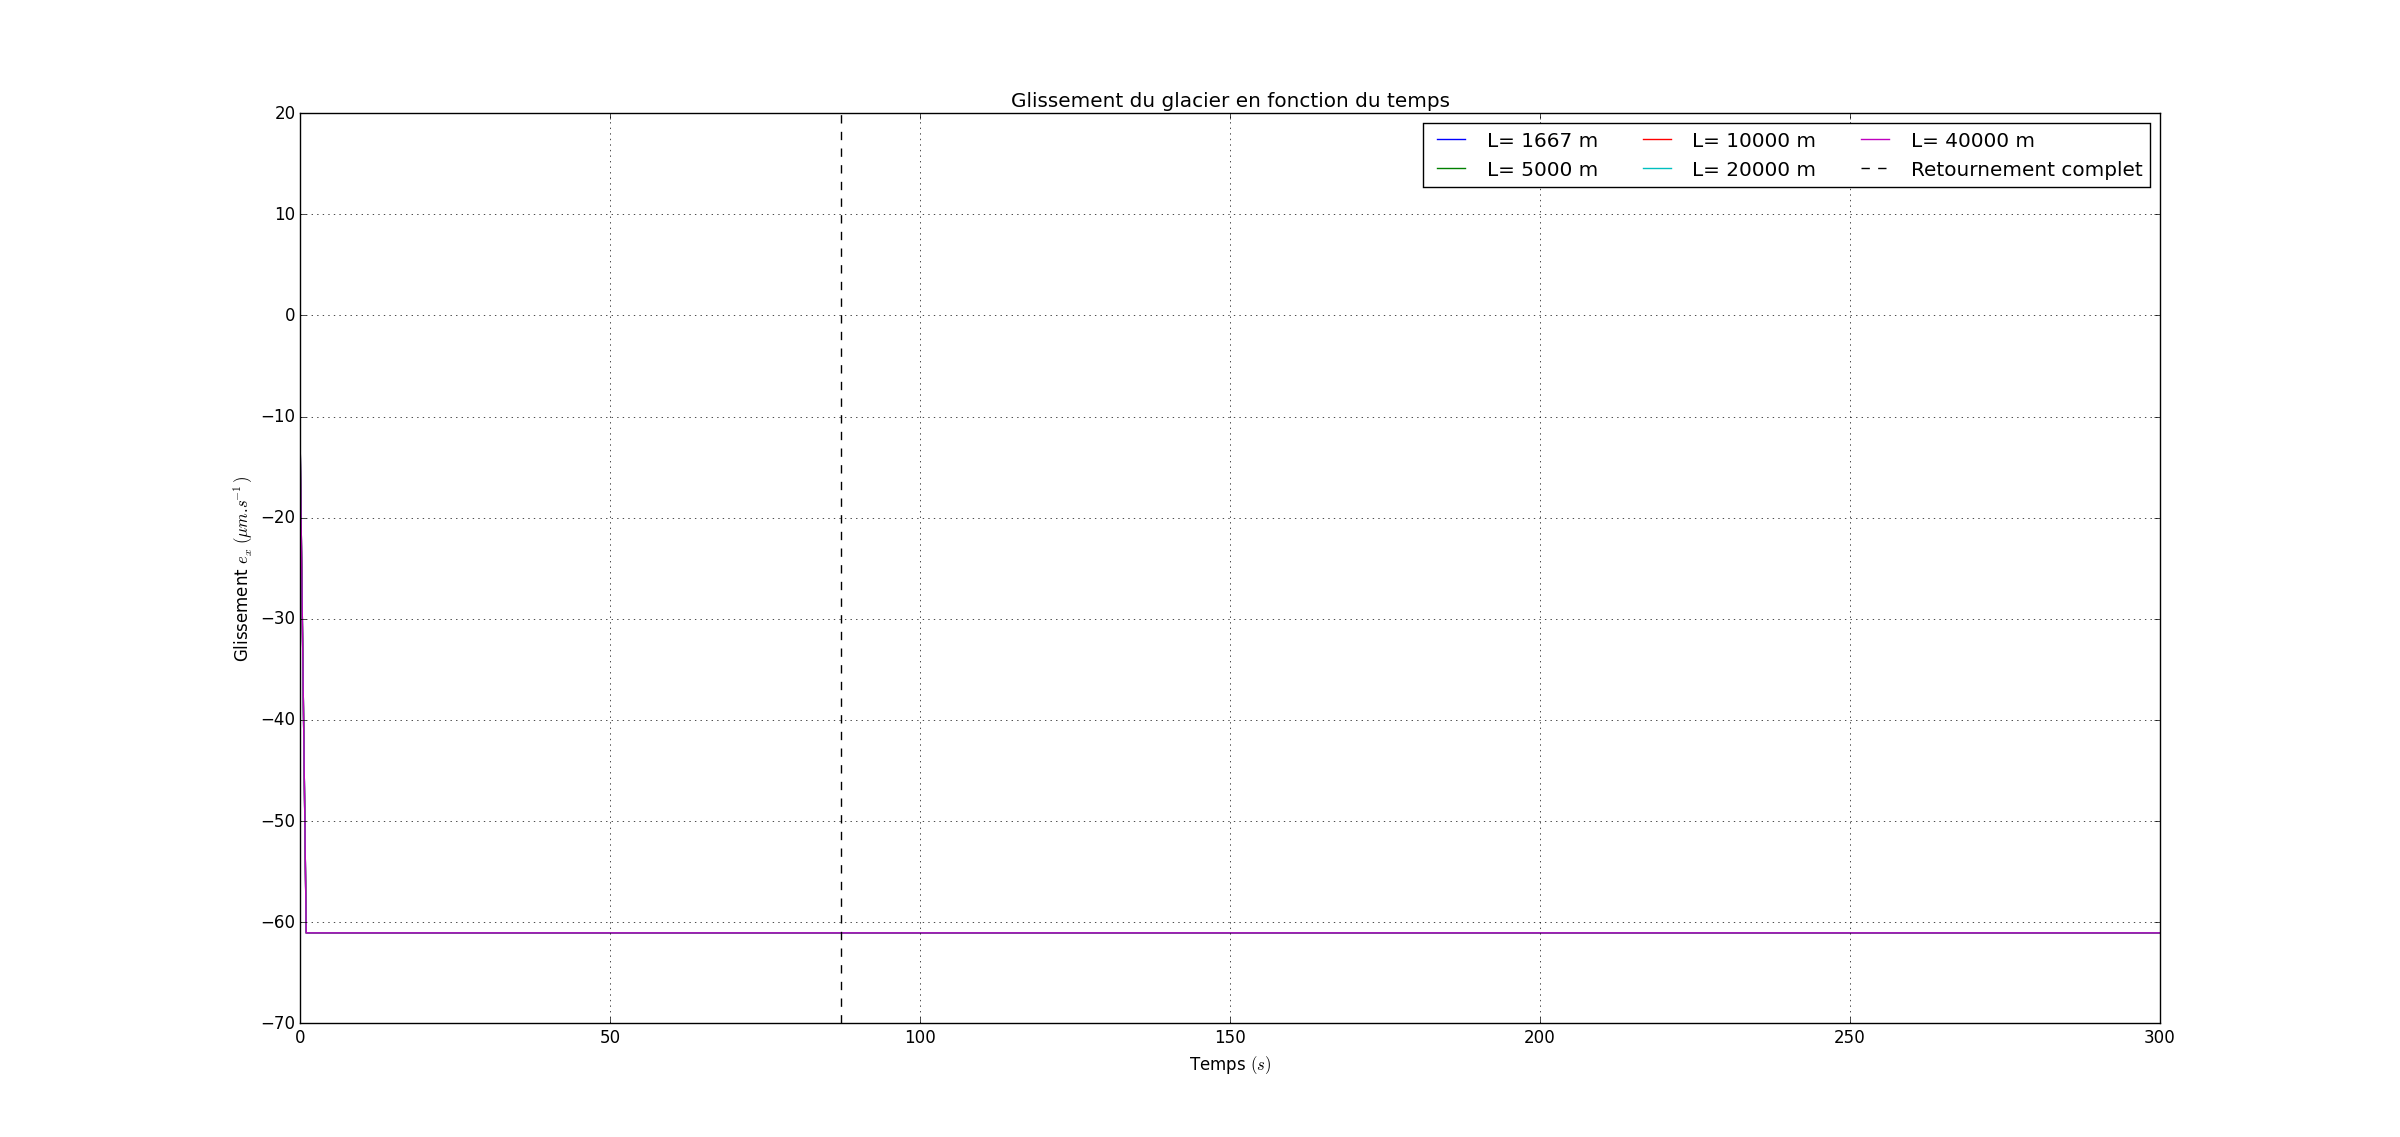
\includegraphics[width=1\linewidth]{figures/Part1/VitesseDt0001.png}
	\caption{Vitesse pour $\delta t= 0.001s$}
	\label{UtdInstable2}
\end{figure}
La figure \ref{UtStableSansPoids} présente les déplacements sans force de perturbation en négligeant l'action du poids, imposant un champ de glissement initial nul au bloc. Le champ de glissement à l'équilibre étant nul, les deux courbes présentées sont identiques. Les blocs ne glissent plus comme pour le modèle précédent.
\\
 
\begin{figure}[h!]
    \centering
    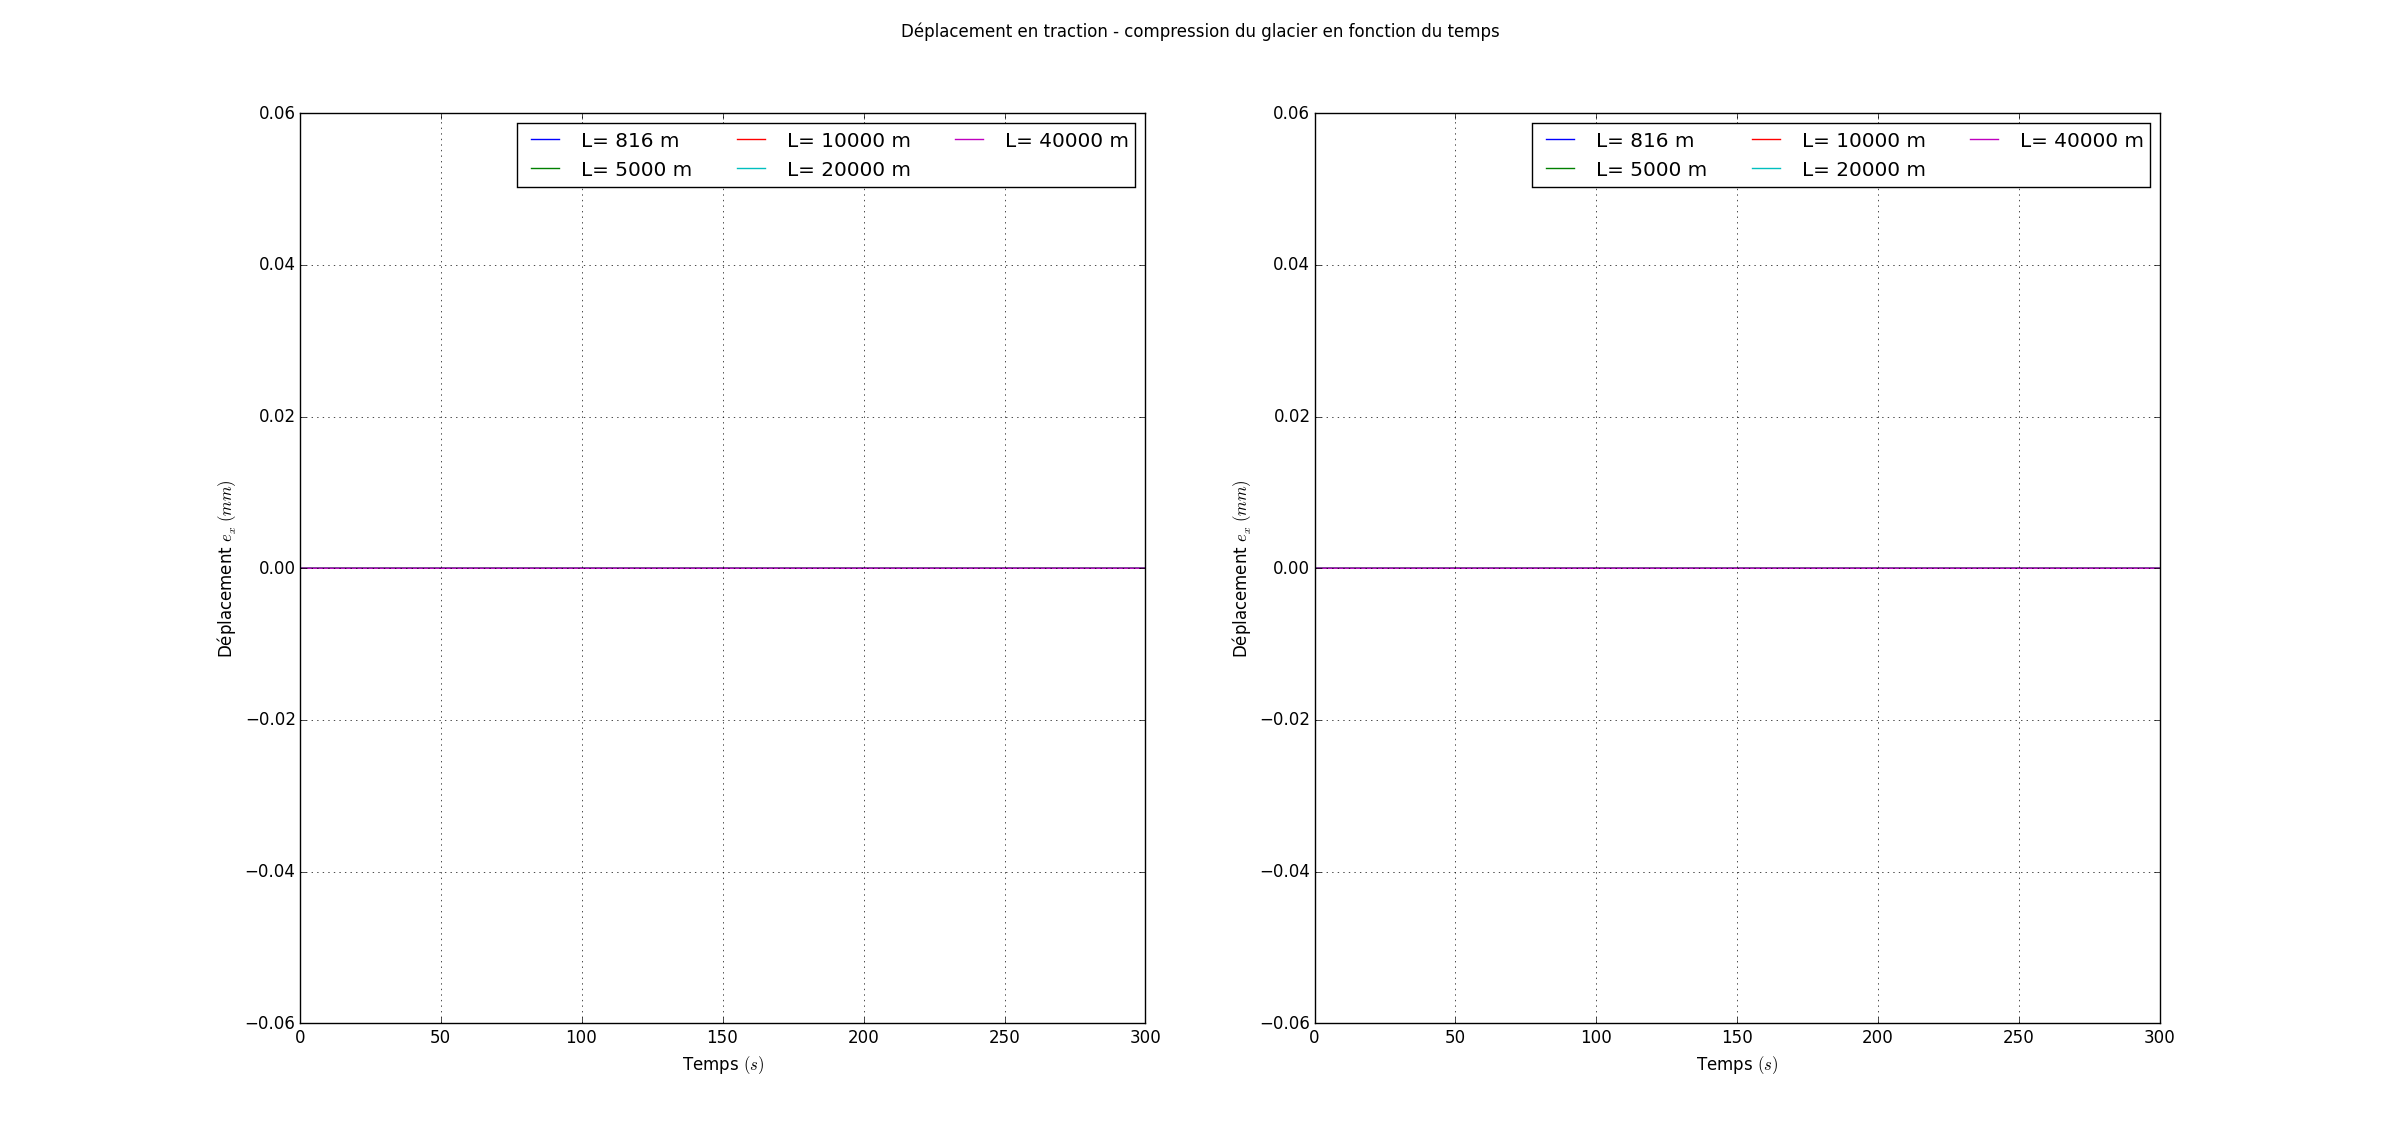
\includegraphics[width=1\linewidth]{figures/Part1/DeplacementDt0012SansPoids.png}
    \caption{Déplacements au cours du temps sans force de perturbation ni glissement initial}
    \label{UtStableSansPoids}
\end{figure}
La dernière figure \ref{UtStableSansPoids} permet de conclure sur l'origine du glissement trop important manifesté figure \ref{UtInstable}. Cela en fait dû à la définition d'un champ initial de glissement non nul et à la non-linéarité de la force de frottement. 
\section{Définition d'un critère de stabilité}
Les champs de vitesse et de déplacement sont calculés à partir du schéma de Verlet. Sa formulation est rappelée formules \ref{UiEq}, \ref{FiEq} et \ref{UdiEq}. 
\\$U_i$ $\dot{U}_i$ et $F_i$ sont respectivement les champs de déplacement, de vitesse et de force à l'intant $t_i$. $[M]$ est la matrice de masse du système. 
\\Les forces considérées dans l'équation \ref{FiEq}, sans perte de généralité, sont la force de frottement ($F_f$) et le poids selon la tangente de la pente ($P_{x'}$). On suppose que la force de frottement suit la loi de Weertman. Le modèle précédent montre que les blocs étant tous identiques géométriquement, leurs vitesses de glissement initiale ou à l'équilibre sont les mêmes.
\\Par la suite nous ne prendrons pas en compte la force élastique ($F_e$) dans le schéma et propagation de l'instabilité. Les blocs glissent à l'équilibre à la même vitesse. Les forces de liaisons entre les blocs peuvent être négligées devant celles de frottement et de poids.
\\ L'action des liaisons entre les blocs étant négligé, nous étudierons seulement le mouvement et la stabilité d'un bloc de longueur $\delta l$. La stabilité de chaque bloc apparaît comme une conditions suffisante à la stabilité du système avec plusieurs blocs. Dans les notations suivantes, les grandeurs suivantes seront des grandeurs scalaires, $U$ le déplacement, $\dot{U}$ la vitesse et $F$ la résultante de force. M est la masse du bloc considéré, $M = M_{bloc} = \rho_{glace} H \delta l $. 
\\ On rappelle la formulation du schéma de Verlet avec les expressions suivantes, \ref{UiEq} \ref{FiEq} et \ref{UdiEq}. $[M]^{-1}$ l'inverse de la matrice de masse est réduit à $\frac{1}{M_{bloc}}$. 
\begin{subnumcases}{}
    U_{i+1} = U_i + \delta t ( \dot{U}_i + \frac{\delta t}{2} [M]^{-1} F_i ) \label{UiEq}  \\
    F_{i+1} = F_f(\dot{U}_{i}) + P_{x'} + F_{perturbation}(t_{i+1}) \label{FiEq} \\
    \dot{U}_{i+1} = \dot{U}_i + \frac{\delta t}{2} [M]^{-1}( F_i + F_{i+1} ) \label{UdiEq} 
\end{subnumcases}
Pour définir la stabilité du système, on cherche d'abord la stabilité en vitesse du schéma d'après l'équation \ref{UdiEq}. On se place à un rang n, rang auquel apparaît la perturbation. Dans la pratique, l'instabilité apparaît des les premières itérations, n  peut être considéré de faible rang. Pour les rangs précédents, la résultante sera prise nulle telle que $\forall i \in \llbracket 1:n \rrbracket, \quad F_i = 0$. De cette façon, le système continue de glisser à la même vitesse qu'à son état initial, c'est à dire $\forall i \in \llbracket 1:n-1 \rrbracket, \quad \dot{U}_i = \dot{U}_0 = \dot{U}_{eq} $. 
\\Le système est stable si les perturbations engendrées au rang n ne sont pas amplifiées par la suite, avec un retour avec une force de perturbation nulle ensuite.  $F_{frottement}(\dot{U}_{eq}) = - F_{poids \ e_{x'}} $, on a bien la résultante des forces nulle, notamment selon le vecteur $\mathbf{e_{x'}}$ tangent à la pente du glacier.
\\

On cherche l'effet de cette perturbation sur la vitesse du système. On se place au rang $n$ dans l'équation \ref{UdiEq}, on introduit une perturbation à la vitesse par rapport à la vitesse d'équilibre ou initiale, notée $\dot{U}_{p \ n}$ telle que:
$$\dot{U}_{n} = \dot{U}_{eq} + \dot{U}_{p \ n} $$
\begin{equation}
	\dot{U}_{n} = \dot{U}_{eq}(1+\epsilon_n) \label{Un1Eq}
\end{equation}
$$ \text{avec} \quad \dot{U}_{p \ n} = \epsilon_n \dot{U}_{eq} \quad \text{et} \quad \epsilon_n \ll 1 $$
\\

On remplace au rang $n+1$ dans l'expression \ref{UdiEq} de la force avec cette valeur de vitesse. De même on trouve:
$$ F_{n+1} = F_{frottement}(\dot{U}_{n}) + F_{poids \ e_{x'}}$$
En considérant que le frottement suit la loi de Weertman, on a: 
\begin{align*}
F_{frottement}(\dot{U}_{n}) &= - sign(\dot{U}_n) C_w \delta l ( | \dot{U}_{n} | )^{\frac{1}{3}} \\
\quad &= - sign(\dot{U}_n) C_w \delta l ( | \dot{U}_{eq} + \dot{U}_{p \ n} | )^{\frac{1}{3}}
\end{align*}
On simplifie cette expression grâce son développement limité à l'ordre 1 en $\dot{U}_{eq}$ en supposant que $\epsilon_n \ll 1$. On suppose que $sign(U_n) = sign(U_{eq}) $. On simplifie alors l'expression du frottement tel que:
\begin{align*}
F_{frottement}(\dot{U}_{n}) &= - sign(\dot{U}_{eq}) C_w \delta l | \dot{U}_{eq} |^{\frac{1}{3}} \left( 1 + \epsilon_n \right)^{\frac{1}{3}} \\
\quad &= - sign(\dot{U}_{eq}) C_w \delta l | \dot{U}_{eq} |^{\frac{1}{3}} \left( 1 + \frac{1}{3} \epsilon_n \right)
\end{align*}
\begin{equation}
F_{frottement}(\dot{U}_n) = F_{frottement}(\dot{U}_{eq}) - \frac{ sign(\dot{U}_{eq}) C_w \delta l}{3} | \dot{U}_{eq}|^{\frac{1}{3}}\epsilon_n
\end{equation}
Dans notre cas on a $sign(\dot{U}_{eq})=-1$, l'ajout d'une perturbation dans le sens de glissement ( selon $- \mathbf{e_{x'}}$) conduit à ajouter une terme de frottement dans la direction opposée (selon $\mathbf{e_{x'}}$). On revenant à l'expression de la résultante des forces au rang $n+1$, on remplace par cette expression de force de frottement. La force de perturbation redevient nulle. On a donc:
\begin{align*}
F_{n+1} &= F_{frottement}(\dot{U}_{n}) + F_{poids \ e_{x'}} \\
\quad &= F_{frottement}(\dot{U}_{eq}) - \frac{ sign(\dot{U}_{eq}) C_w \delta l}{3} | \dot{U}_{eq}|^{\frac{1}{3}}\epsilon_n + F_{poids \ e_{x'}}
\end{align*}
On simplifie avec $F_{poids \ e_{x'}} = - F_{frottement}(\dot{U}_{eq})$, on obtient finalement:
\begin{equation}
F_{n+1}= - \frac{ sign(\dot{U}_{eq}) C_w \delta l}{3} | \dot{U}_{eq}|^{\frac{1}{3}}\epsilon_n \label{Fn1Eq}
\end{equation}
On revient enfin à l'expression de la vitesse avec l'expression \ref{UdiEq} au rang suivant $n+1$. On défini alors la vitesse de perturbation au rang $n+1$ par rapport à la vitesse d'équilibre initiale notée $\dot{U}_{p \ n+1}$.
\begin{equation}
\dot{U}_{n+1} = \dot{U}_{n} + \frac{\delta t}{2 \rho_{glace} H \delta l } \left( F_n + F_{n+1} \right) 
\end{equation}
On simplifie avec $F_n = 0$. On remplace $F_{n+1}$ par l'expression \ref{Fn1Eq} et $\dot{U}_n$ avec l'expression \ref{Un1Eq}. On a finalement:
\begin{equation}
\dot{U}_{n+1} = \dot{U}_{eq} + \dot{U}_{p \ n } - \frac{sign(\dot{U}_{eq}) C_w\delta t}{6 \rho_{glace} H} |\dot{U}_{eq}|^{\frac{1}{3}} \epsilon_n 
\end{equation}
On exprime le terme de perturbation au rang $n+1$ induit par $\epsilon_n$. $\epsilon_{n+1}$ est simplement la perturbation induite par $\epsilon_n$, on considère alors que seule cette perturbation apparaît.
\begin{equation}
\dot{U}_{n+1} = \dot{U}_{eq} + \dot{U}_{p \ n} + \dot{U}_{p \ n+1} = \dot{U}_{eq} (1+\epsilon_n +\epsilon_{n+1})
\end{equation}
Avec: 
$$ \epsilon_{n+1} = - \frac{sign(\dot{U}_{eq}) C_w\delta t}{6 \rho_{glace} H} \frac{|\dot{U}_{eq}|^{\frac{1}{3}} }{\dot{U}_{eq}} \epsilon_n $$
Pour $sign(\dot{U}_{eq})=-1$, on a $\dot{U}_{eq} = - |\dot{U}_{eq} |$. En remplaçant dans l'expression précédente on trouve:
\begin{equation}
\epsilon_{n+1} = - \frac{C_w\delta t}{6 \rho_{glace} H} |\dot{U}_{eq}|^{-\frac{2}{3}} \epsilon_n \label{Epsin1Eq}
\end{equation}
On remarque que la perturbation $\epsilon_{n+1}$ est de signe opposé à $\epsilon_{n}$. Pour que le schéma reste stable, que la perturbation ne grandisse pas il faut que le perturbation $\epsilon_{n+1}$ soit inférieur à $\epsilon_n$ en module. De cette façon, la perturbation est lissée, physiquement dû à l'action du frottement s'opposant au mouvement mais ne pouvant pas accélérer le système dans le sens opposée au glissement initiale. Le système doit donc vérifier la condition suivante:
$$ | \epsilon_{n+1} | < 2 | \epsilon_n | $$
En remplaçant par l'expression \ref{Epsin1Eq} et en simplifiant par $\epsilon_n$ des deux cotés, on trouve :
$$ \frac{C_w\delta t}{6 \rho_{glace} H} |\dot{U}_{eq}|^{-\frac{2}{3}} < 2 $$
En gardant le pas $\delta t$ d'un coté de l'inégalité, on a :
\begin{equation}
\delta t < \frac{12 \rho_{glace} H } {C_w} |\dot{U}_{eq} |^{\frac{2}{3}} \label{DtIneq}
\end{equation}
On en déduit l'existence d'une limite de stabilité pour le pas de temps $\delta t$. On notera cette limite $\delta t_{stable}$. On a finalement d'après l'inégalité \ref{DtIneq}:
\begin{equation}
\delta t_{stable} = \frac{12 \rho_{glace} H } {C_w} |\dot{U}_{eq} |^{\frac{2}{3}} \label{DtStableEq}
\end{equation}
\\
 
Cette expression ne dépend pas de la dimension des blocs $\delta l$. Elle dépend en revanche de la vitesse initiale et du paramètre de friction $C_W$.
\\ 

En utilisant $H = 800m$, $\rho_{glace} = 920 kg.m^{-3}$, $C_W = 5.623 \ 10^6 Pa$ et $\dot{U}_{eq} = -1.125 \ 10^{-5}m.s^{-1}$, après application numérique on trouve $\mathbf{\delta t_{stable} = 0.0008s}$. 
\\

Les figures \ref{UendDtLoop} et \ref{FsismiqueDtLoop}, les courbes respectivement du déplacement final et des efforts de contact en fonction du pas de temps $\delta t$, confirme l'influence du pas de temps sur les résultats du système. La limite de stabilité $\delta t_{stable}$ est repérée en gras par des droites verticale, sur les figures \ref{UendDtLoop} et \ref{FsismiqueDtLoop}. 
\\

L'amplitude du déplacement perturbé semble être inversement proportionnel au pas de temps $\delta t$, pour $\delta t > \delta t_{stable}$. Un changement de régime de stabilité est perçu avec la figure \ref{UendDtLoop}; l'amplitude chute brutale autour de $\delta t_{stable}$. De même pour le graphique \ref{FsismiqueDtLoop}, la force sismique diminue linéairement avec le pas de temps, puis devient totalement nulle pour $\delta t < \delta t_{stable}$, lorsque le pas de temps atteint la limite de stabilité. Les dernière valeurs de force sismique ne sont pas affichées car nulles, ce qui est effectivement le cas en l'absence de chargement extérieur ou de force de contact. Cela est un témoin de la convergence du système.
\\

Pour revenir au figures initiales \ref{UtdInstable} et  \ref{UtdInstable2}, le dépassement de $\delta t_{stable}$ peut en effet entraîner des oscillations pour le système en vitesse. On l'observe particulièrement sur la figure \ref{UtdInstable2} où le dépassement par rapport à $\delta t_{stable}$ est plus important. Toutefois, comme le montre la figure \ref{UtdInstable}, le dépassement de $\delta t_{stable}$ n'entraîne pas nécessairement des oscillations, simplement un glissement incontrôlé du glacier. Le système n'est toujours pas à l'équilibre.
\begin{figure}[h!]
    \centering
    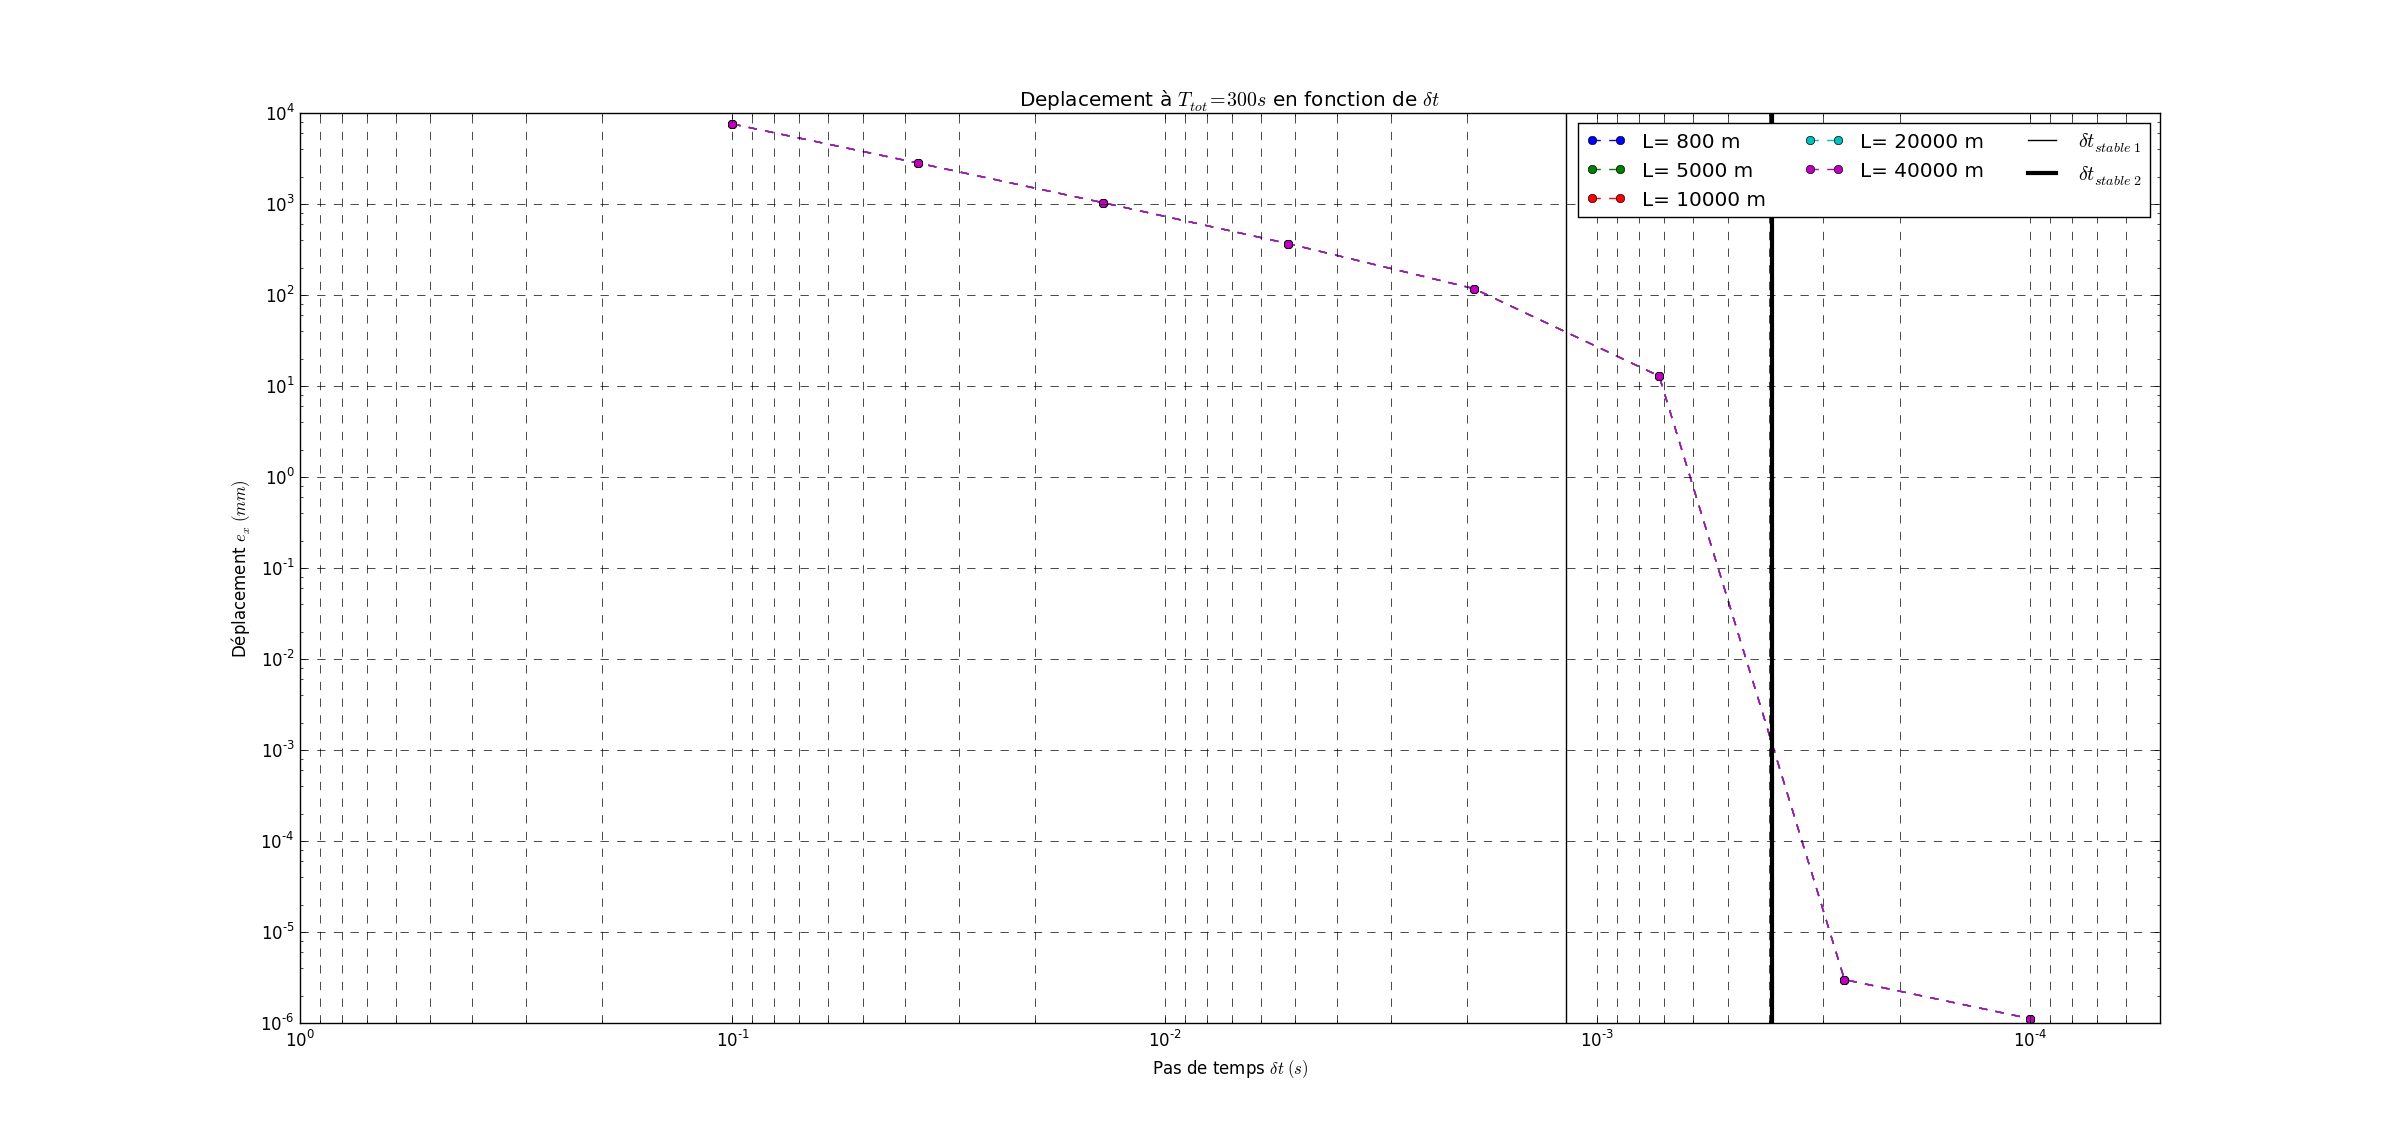
\includegraphics[width=1\linewidth]{figures/Part2/Deplacement.png}
    \caption{Amplitude du déplacement perturbé finale (à $T_{tot} = 300s$) en fonction du pas de temps $\delta t $}
    \label{UendDtLoop}
\end{figure}
\begin{figure}[h!]
    \centering
    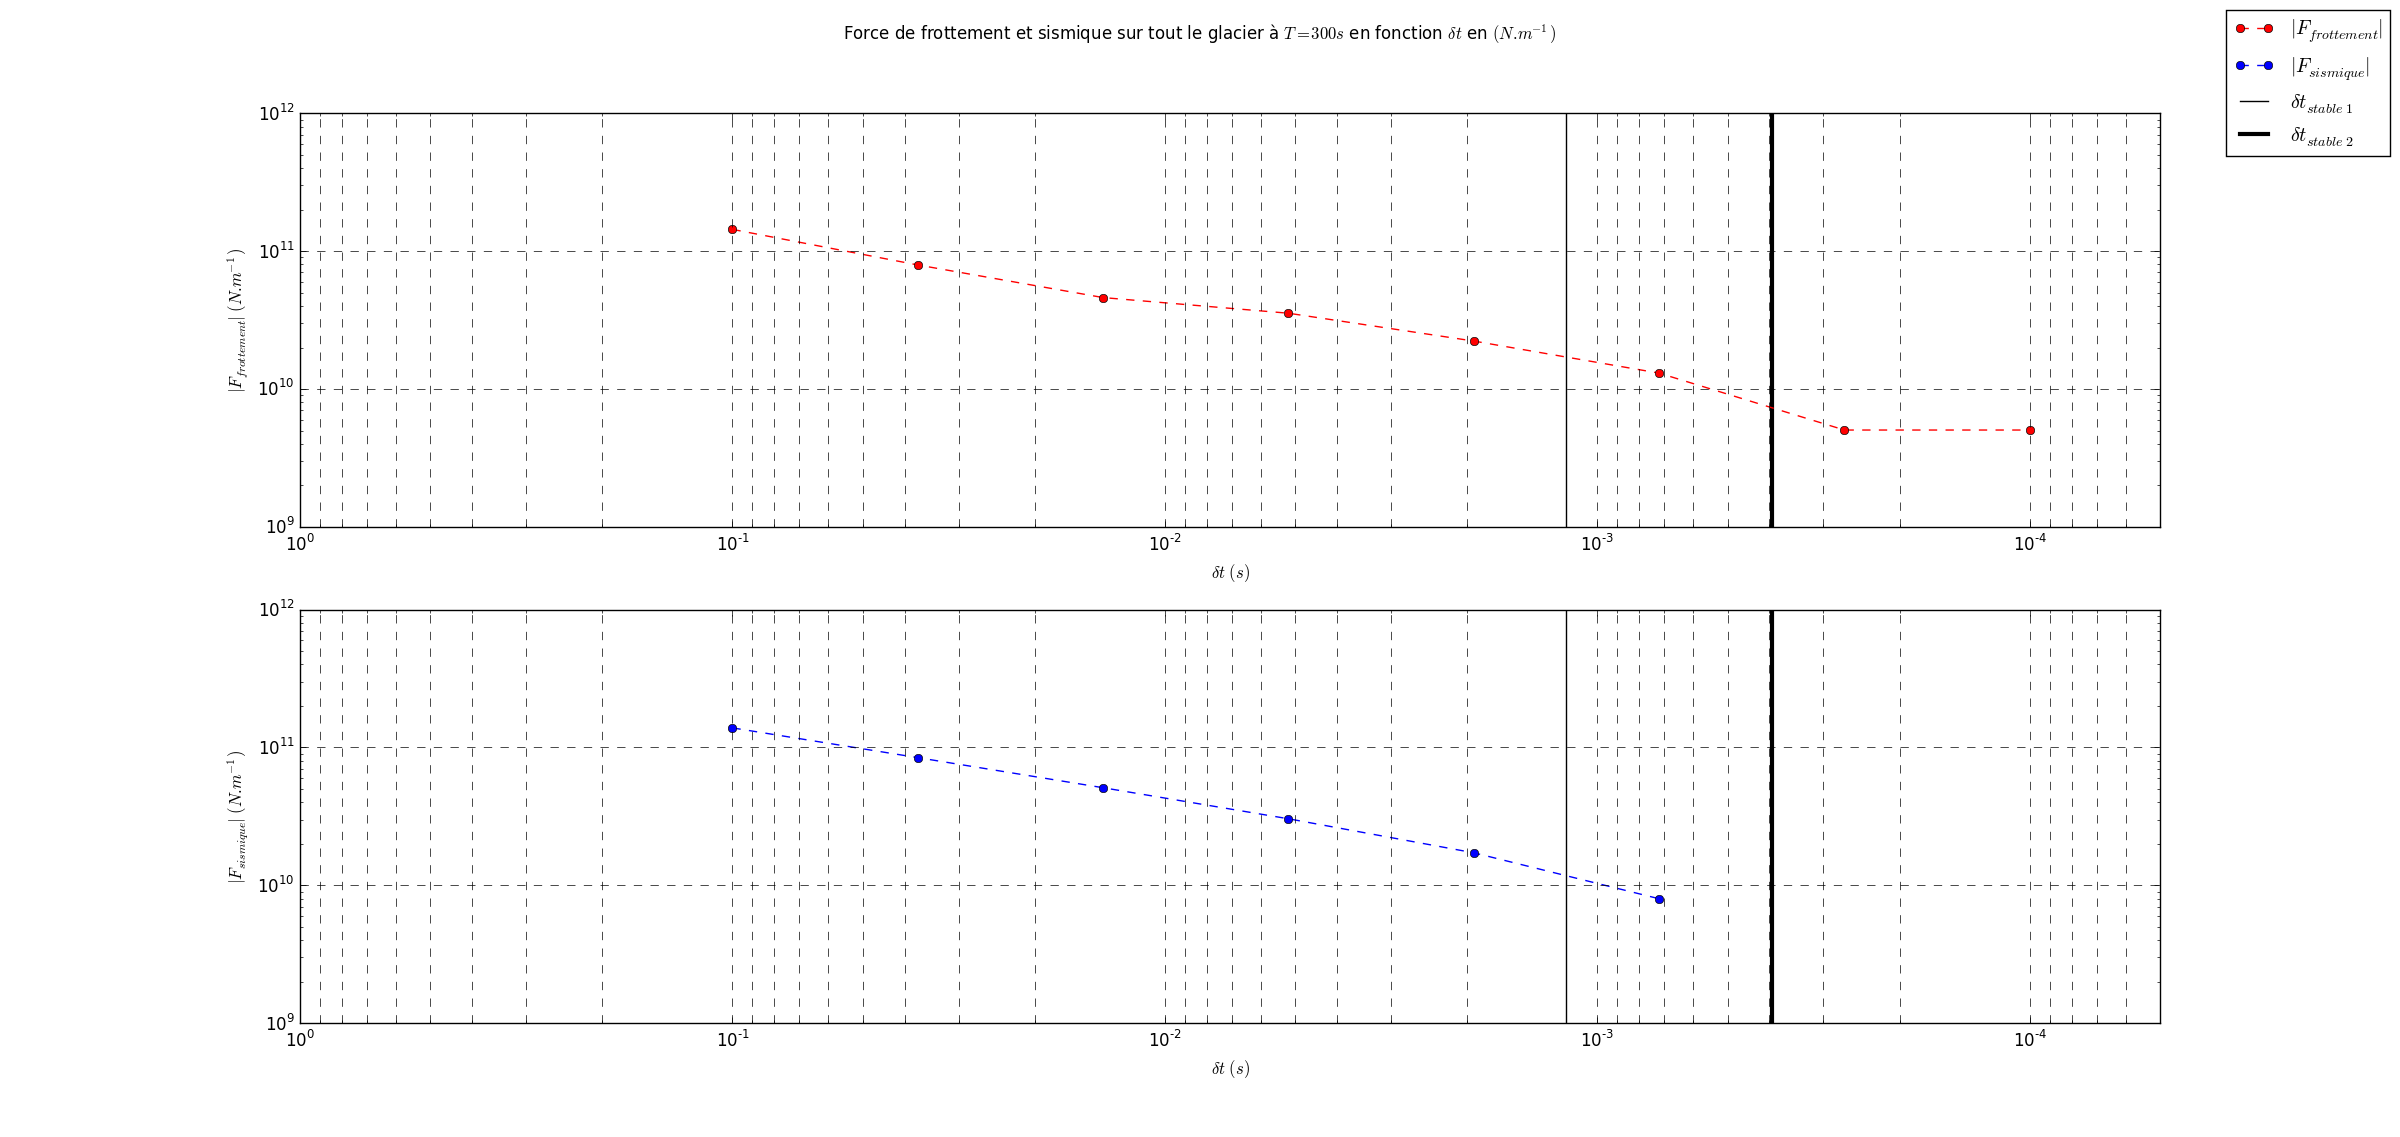
\includegraphics[width=1\linewidth]{figures/Part2/ForcesFrottement.png}
    \caption{Magnitude de la force de frottement finale en fonction du pas de temps $\delta t$}
    \label{FsismiqueDtLoop}
\end{figure}
Avec la figure \ref{TpsComputeDtLoop}, le temps de calcul est inversement proportionnelle au pas de temps. Il est proportionnel au nombre d'itération, la contrepartie de la convergence du modèle.
\begin{figure}[h!]
    \centering
    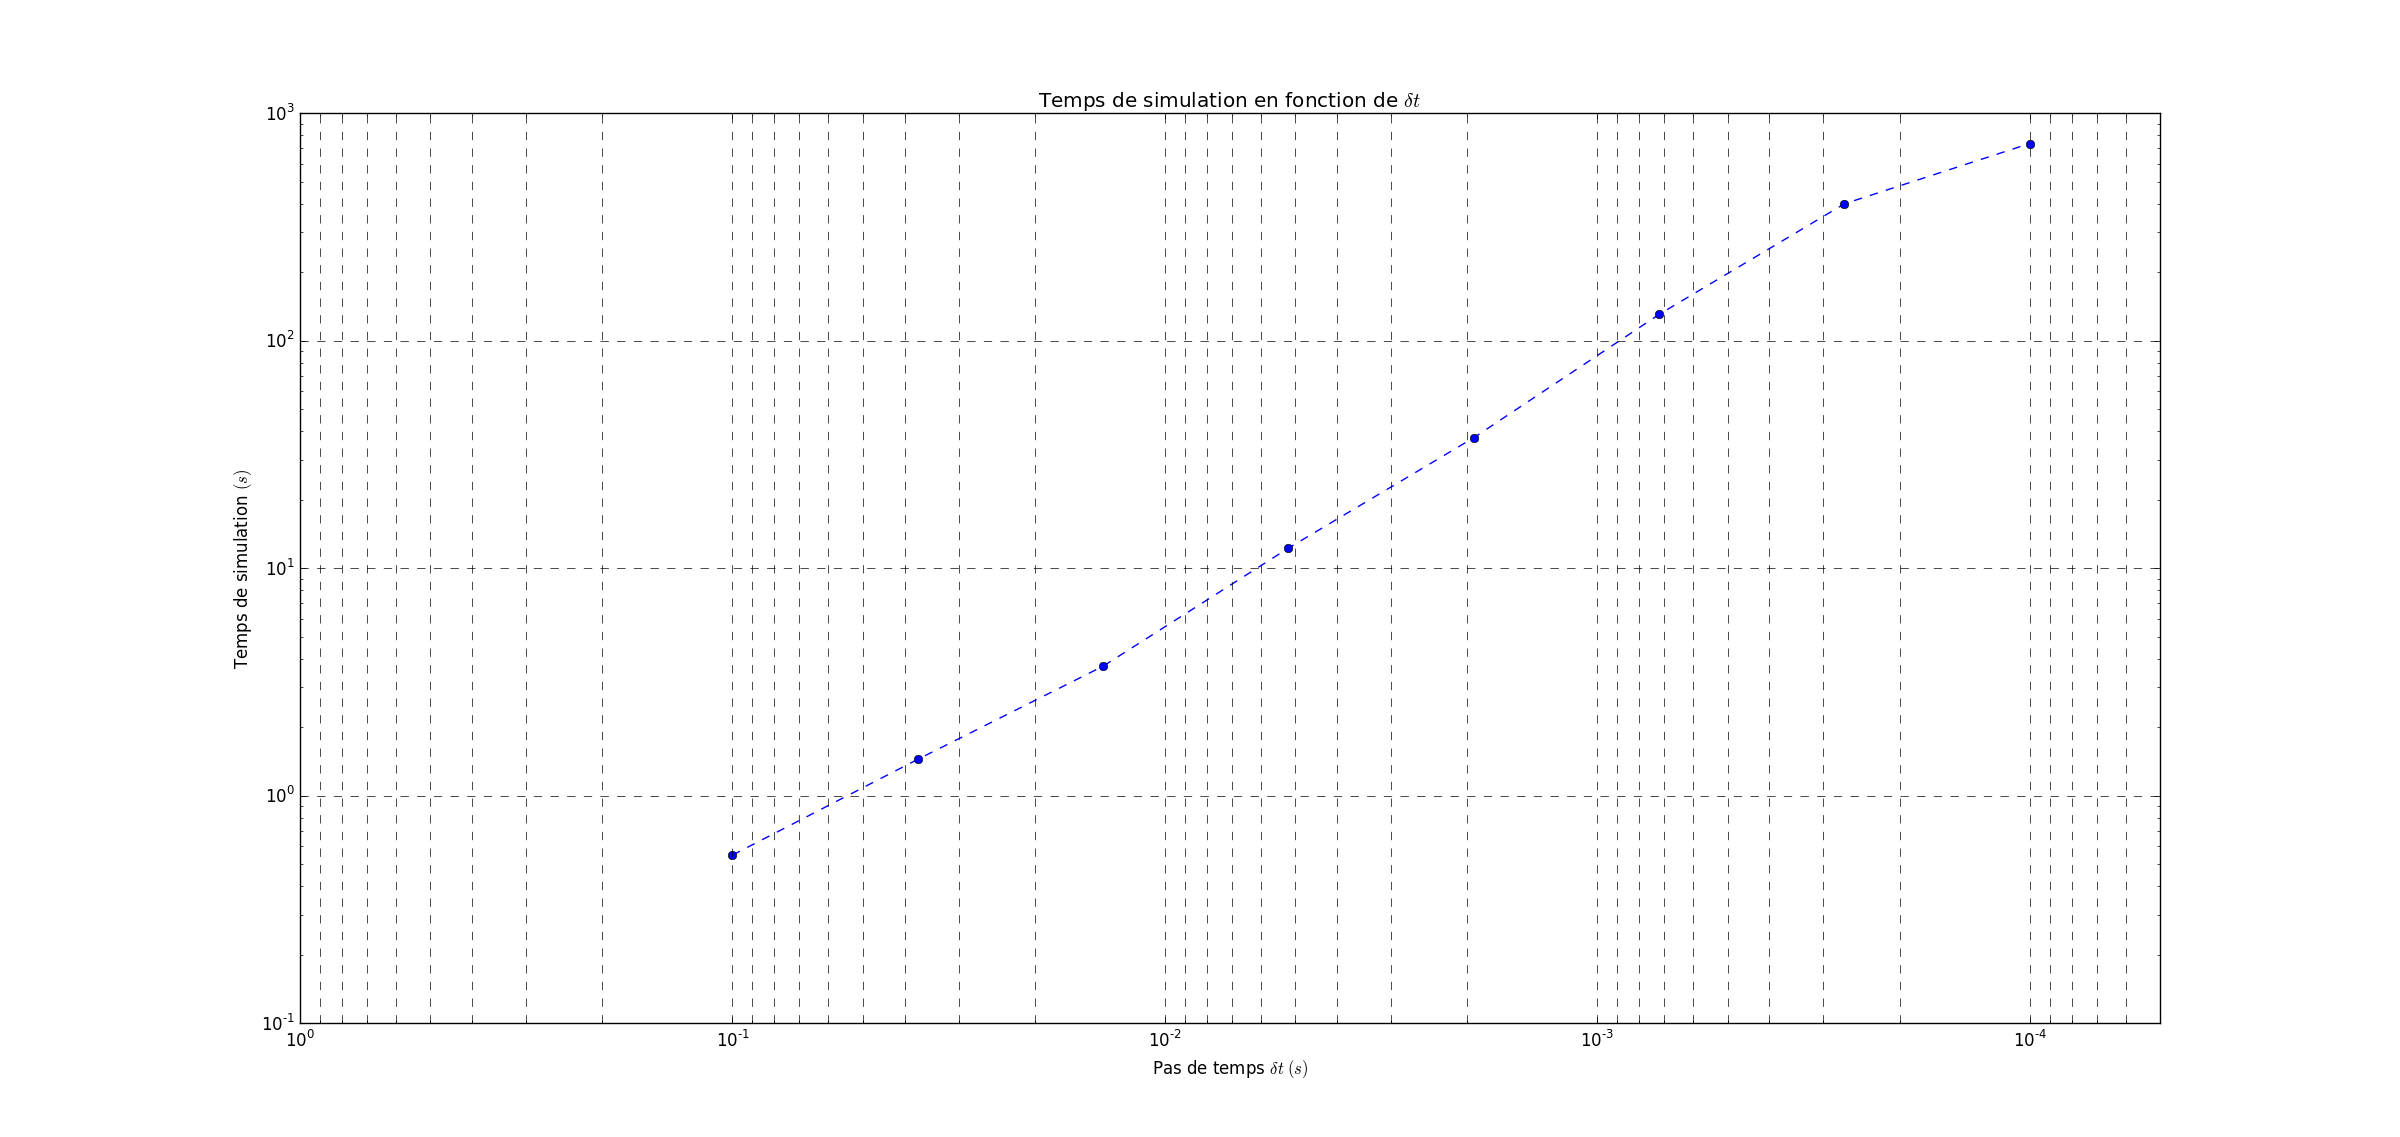
\includegraphics[width=1\linewidth]{figures/Part2/TempsCalcul.png}
    \caption{Temps de calcul en fonction du pas de temps $\delta t$}
    \label{TpsComputeDtLoop}
\end{figure}
\section{Paramètres retenus et résultats}

\subsection{Test stable avec $\delta l =500$ et $L_{tot} = 40km$}
Les figures suivantes sont les résultats du modèle calculé avec un pas de temps $\delta t =0.0002s$, inférieur à $\delta t_{stable}$. On cherche l'influence de la force de contact sur le modèle, et la stabilité du système.
\\

Les figures suivantes illustreront les résultats avec l'ajout d'une force de perturbation. Le modèle reste conditionnellement stable en fonction de la vitesse de glissement des blocs et c'est ce que nous pourrons observer à travers ces résultats. Il faut tout d'abord rappeler que nous reprenons les paramètres géométriques \ref{PaSimuInsta} de la première section. La longueur totale est notamment de $L_{tot} = 40km$, et la taille des blocs est de $\delta l = 500m$. 
\\ Le temps de simulation est toutefois réduit à $T_{tot} = 100s$. Le but de cette simulation est uniquement d'observer si le schéma devient stable, et notamment à sont maximum de vitesse.
\\

\begin{figure}
	\centering
	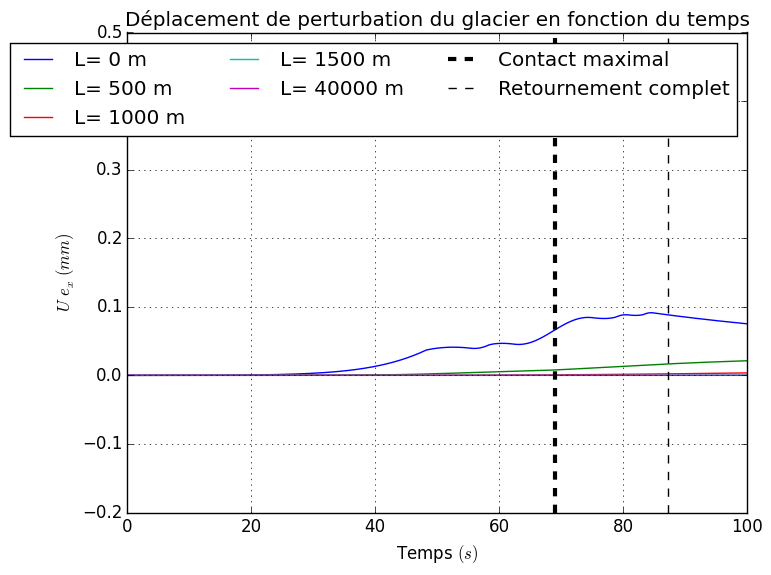
\includegraphics[width=0.5\linewidth]{figures/Part3/Subpart1/Deplacement.png}
	\caption{Déplacement aux premiers points du glacier au cours du retournement d'iceberg}
	\label{UtInstablePart3}
\end{figure}
Le déplacement au premier bloc présente des irrégularités (figure \ref{UtInstablePart3}) qui sont relevées par le comportement en vitesse du système figure \ref{UtdInstablePart3}. Le comportement en vitesse semble atteindre une limite de stabilité en fonction de sa vitesse, mais redevient stable à partir d'une autre. 
\\

Le même comportement est observé figure \ref{FsisInstablePart3} avec la force sismique sur tout les blocs. 

\begin{figure}
	\centering
	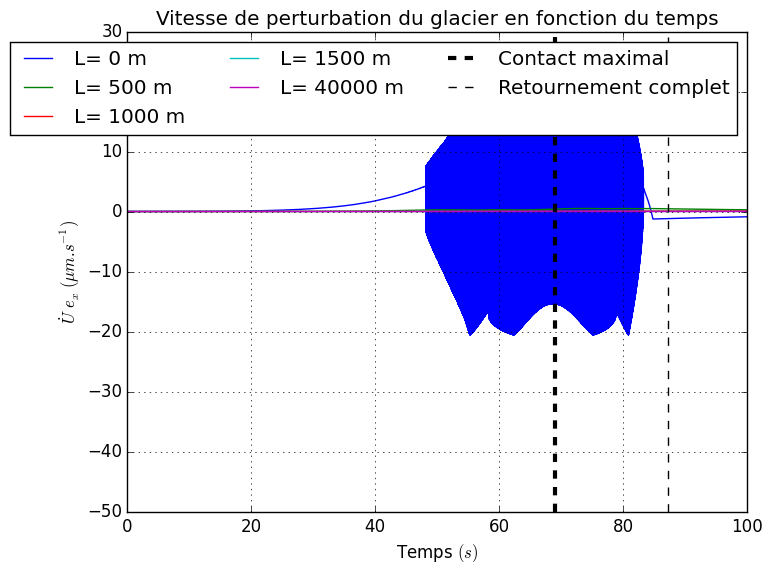
\includegraphics[width=0.5\linewidth]{figures/Part3/Subpart1/Vitesse.png}
	\caption{Vitesse aux premiers points du glacier au cours du retournement d'iceberg}
	\label{UtdInstablePart3}
\end{figure}

\begin{figure}
	\centering
	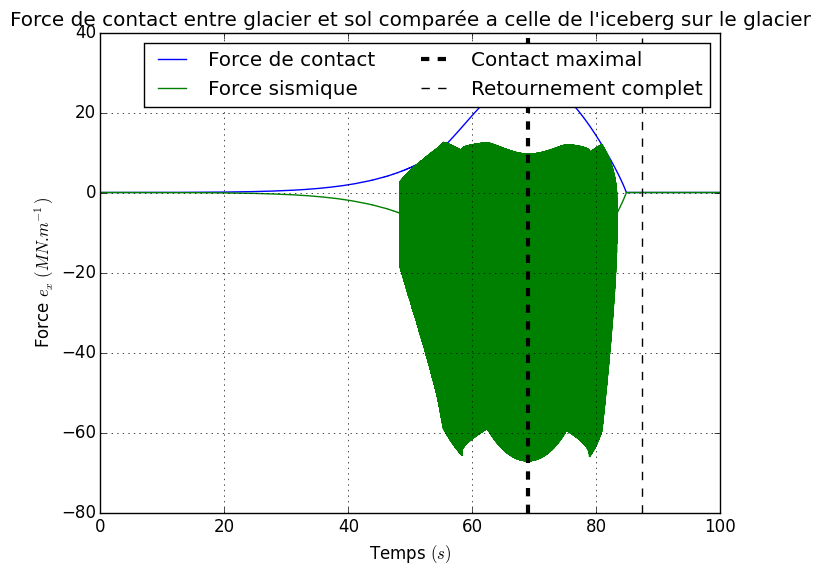
\includegraphics[width=0.5\linewidth]{figures/Part3/Subpart1/Fsismique.png}
	\caption{Force sismique des premiers blocs du glacier contre le lit rocheux au cours du retournement d'iceberg}
	\label{FsisInstablePart3}
\end{figure}

\subsection{Etude du domaine de stabilité en vitesse}

Les figures \ref{UtdInstablePart3} et \ref{FsisInstablePart3} relèvent la présence d'un domaine de stabilité en vitesse. La formule \ref{DtStableEq} permet d'obtenir le domaine stabilité en vitesse à l'état d'équilibre. Ce critère n'est plus respecté forcément respecté lorsque la vitesse diminue. 
\begin{equation}
	\label{DtStableUminEq}
	\delta t_{stable \ W} = \frac{12 \rho_{glace} H}{C_W} \left( min(|\dot{U}|) \right)^{\frac{2}{3}} 
\end{equation}
\\

En supposant que la vitesse reste négative, le glissement du glacier orienté dans la direction avale, le pas de temps est commandé par le maximum de la vitesse à priori.
\\ Le problème reste ouvert lorsque que la vitesse s'annule. Le pas de temps $\delta t_{stable}$ risque de s'annuler également, donnant un temps de calcul infini. 
\\ Dans le cas précédent en considérant $\delta t_{stable} = 0.0002s$, le schéma devient instable pour des vitesses comprises telles que $| \dot{U}(t) | \leq 4.06 \ 10^{-6} m.s^{-1} $.  
\\

Une solution pour réduire ces instabilités pour les faibles vitesse est de régulariser la force de frottement. On utilise alors la loi décrite avec la formule suivante \ref{FfrictionRegExp}.
\begin{equation}
	\label{FfrictionRegExp}
	F_{f \ lineaire} = \left\{ \begin{array}{cl} 
	- sign(\dot{U}) C_w \delta l \left( | \dot{U} | \right)^{\frac{1}{3}} & \text{si } | \dot{U} | \geq \nu \\
	- C_l \delta l \dot{U} & \text{sinon} 
	\end{array} \right .
\end{equation}
L'expression dépend d'une limite $\nu$, qui définit la frontière entre les domaines linéaires et non-linéaire de la loi. Ce paramètre est définie positive. 
\\ On veut que la loi soit continue en $\nu$. On trouve alors l'expression du coefficient $K$ valable en $\dot{U} = - \nu$ et $\dot{U} = \nu$. Son expression est donnée formule \ref{KExp}.
\begin{equation}
	\label{KExp}
	C_l = C_w \nu^{-\frac{2}{3}}
\end{equation}
Il faut s'assurer toutefois que cette loi n'engendre pas des instabilités similaires à la loi de frottement de Weertman. On reprend l'étude de la partie précédente avec cette nouvelle loi de frottement.
\\

Pour s'assurer de la stabilité du schéma on reprend donc les équations \ref{UiEq}, \ref{FiEq} et \ref{UdiEq} avec cette nouvelle loi de frottement en supposant que la vitesse considérée est telle que $| \dot{U} | < \nu$.
\\ On considère seulement le mouvement d'un bloc sans interaction de liaison élastique. On se place à un rang $n$ décrit avec les équations \ref{FnEqPart3} et \ref{UnEqPart3} en force et en vitesse. On fait intervenir la composante tangentielle du poids, la force de frottement (se servant de la vitesse au rang précédent $\dot{U}_{n-1}$) et la force de perturbation. Le schéma est linéaire , on ne considère uniquement la propagation de la perturbation sans influence de force.
\begin{subnumcases}{}
	F_n = F_f(\dot{U}_{n-1}) + P_{poids \ \mathbf{e_x'}} + F_{perturbation}(t_n) = 0
	\label{FnEqPart3} \\
	\dot{U}_n = \dot{U}_{n-1} (1+\epsilon_n)\label{UnEqPart3}
\end{subnumcases}
On cherche alors l'évolution de la perturbation $\epsilon_{n}$ au rang $n+1$, sans influence ou changement de la force de perturbation. On suppose $F_{perturbation}(t_n) = F_{perturbation}(t_{n+1})$.
\\ On applique la suite du schéma de Verlet au rang $n+1$. On trouve donc les relations suivantes avec l'hypothèse d'invariance de la force de perturbation.
\begin{align*}
	F_n & = F_f(\dot{U}_{n}) + P_{poids \ \mathbf{e_x'}} + F_{perturbation}(t_n) \\
	\quad & = - F_f(\dot{U}_{n-1}(1+\epsilon_{n})) + P_{poids \ \mathbf{e_x'}} + F_{perturbation}(t_n) 
\end{align*}
Par linéarité de la loi de frottement, on peut séparer  $ F_f(\dot{U}_{n-1}(1+\epsilon_{n})) = F_f(\dot{U}_{n-1}) + F_f( \dot{U}_{n-1} \epsilon_{n}) $. On retrouve l'expression de la force au rang $n$. On peut donc simplifier l'expression, et donner:
\begin{equation}
	\label{Fn1Part3}
	F_n = - C_l \delta l \dot{U}_{n-1} \epsilon_{n}
\end{equation} 
On cherche à présent l'expression de la vitesse $\dot{U}_{n+1}$ au rang $n+1$. 
\begin{align*}
	\dot{U}_{n+1} &= \dot{U}_n(1+\epsilon_{n}) + \frac{\delta t}{2 \rho_{glace} H \delta l} (F_n + F_{n+1} ) \\
	\quad &= \dot{U}_n (1 + \epsilon_{n} - \frac{\delta t K }{2 \rho_{glace} H } \epsilon_n ) 	
\end{align*}
On en déduit l'expression de la perturbation au rang $n+1$, avec les formules \ref{Un1EqPart3} et \ref{Epsin1Eq}.
\begin{equation}
	\dot{U}_{n+1} = \dot{U}_n (1+ \epsilon_n + \epsilon_{n+1})
	\label{Un1EqPart3}
\end{equation}
Avec la perturbation $\epsilon_{n+1}$:
\begin{equation}
	\label{Epsn1Eq}
	\epsilon_{n+1} = - \frac{\delta t C_l }{2 \rho_{glace} H } \epsilon_n 
\end{equation}
D'après l'expression de $\dot{U}_{n+1}$ formule \ref{Un1EqPart3}, on veut $ |\epsilon_{n+1} | < 2 | \epsilon_n |$.
\\ On trouve finalement l'expression de la limite de stabilité en temps pour la loi de frottement linéaire, formule \ref{DtstableLin}.
\begin{equation}
	\delta t_{stable \ lineaire} = \frac{4 \rho_{glace} H }{C_l}
	\label{DtstableLin}
\end{equation}
\\

On cherche à comparer avec la limite de stabilité avec la loi de Weertman. Pour cela le coefficient $C_l$ est remplacé avec son expression \ref{KExp}. La frontière en vitesse des lois de frottement $\nu$ dans \ref{KExp} est définie avec la limite de stabilité en vitesse de la loi de Weertman ($min ( | \dot{U} | ) $ dans \ref{DtStableUminEq}). Cette limite est désormais notée $\dot{U}_{lim \ stable}$. 
\begin{align*}
	\nu &= \gamma \dot{U}_{lim \ stable} \quad \text{avec } \gamma \geq 1 \\
	\quad &= \gamma \left( \frac{\delta t_{stable \ W} C_W }{12 \rho_{glace} H} \right)^{\frac{3}{2}}
\end{align*}
On trouve alors l'expression du coefficient $K$, en remplaçant $\nu$ dans \ref{KExp} avec cette expression. 
\begin{equation}
	C_l = \frac{12 \rho_{glace} H }{\delta t_{stable \ W}} \gamma^{- \frac{2}{3}}
	\label{KExp2}
\end{equation}
En remplaçant $C_l$ dans l'expression \ref{DtstableLin} de $\delta t_{stable \ lineaire}$, on trouve finalement suivante pour la limite de stabilité de la loi linéaire:
\begin{equation}
	\delta t_{stable \ lineaire} = \frac{\delta t_{stable \ W} }{6} \gamma^{\frac{2}{3}}
	\label{DtStLin2}
\end{equation}
\\

On remarque que lorsque $\gamma = 1$, $\nu = \dot{U}_{lim \ W}$, et que la loi de frottement utilisée est la plus proche de la loi de Weertman, on a $\delta t_{stable \ lineaire} = \frac{\delta t_{stable \ W} }{6}$. Le critère de stabilité de la loi linéaire est plus fort dans ce cas que celui pur la loi de Weertman. Cela assure toutefois la stabilité du schéma pour n'importe quelle vitesse. 
\subsection{Résultats et observation de stabilité avec la loi régularisée}
On prend désormais en compte la loi de frottement régularisé \ref{FfrictionRegExp}, avec les perturbations. Pour étudier la stabilité du schéma, on modélise seulement le mouvement d'un bloc de longueur $\delta l$ et hauteur $H$, en contact avec l'iceberg et sans interaction élastique d'autre bloc. Le glacier est alors réduit à un bloc. 
\\

Le programme de calcul définit tout d'abord la vitesse à l'équilibre du système $\dot{U}_{eq}$. La limite du domaine linéaire de la loi de frottement est alors définie par rapport à cette vitesse, telle que $\nu = \eta \dot{U}_{eq}$. On calcule ensuite le pas de temps à partir de $\delta t_{stable \ lineaire}$ et de la formule \ref{DtStLin2} et \ref{DtStableUminEq} en prenant $min(|\dot{U}|) = \nu$. On fixe finalement le pas de temps du système à $\delta t = \frac{\delta t_{stable \ lineaire} }{a} $ avec $a \geq 1$ pour se placer en dessous de cette limite de stabilité. 
\\

On considèrera $\eta= 0.1$ pour la définition de la limite $\nu$. On teste plusieurs valeurs de coefficient $a$ et mettre en évidence de comportement instable du domaine linaire de la loi de frottement.
\\
\\
\underline{Test avec $\delta t > delta t_{stable \ lineaire}$} :
\\

Pour cette première étude on se place dans le domaine de stabilité de la loi de frottement Weertman, mais avec le pas de temps supérieur à la limite de stabilité de la partie linéaire. 
\\ Le but de cette étude étant d'observer les phénomènes d'instabilité du à la partie linéarisée de la loi de frottement. 
\\
\\
\begin{figure}[h!]
	\centering
	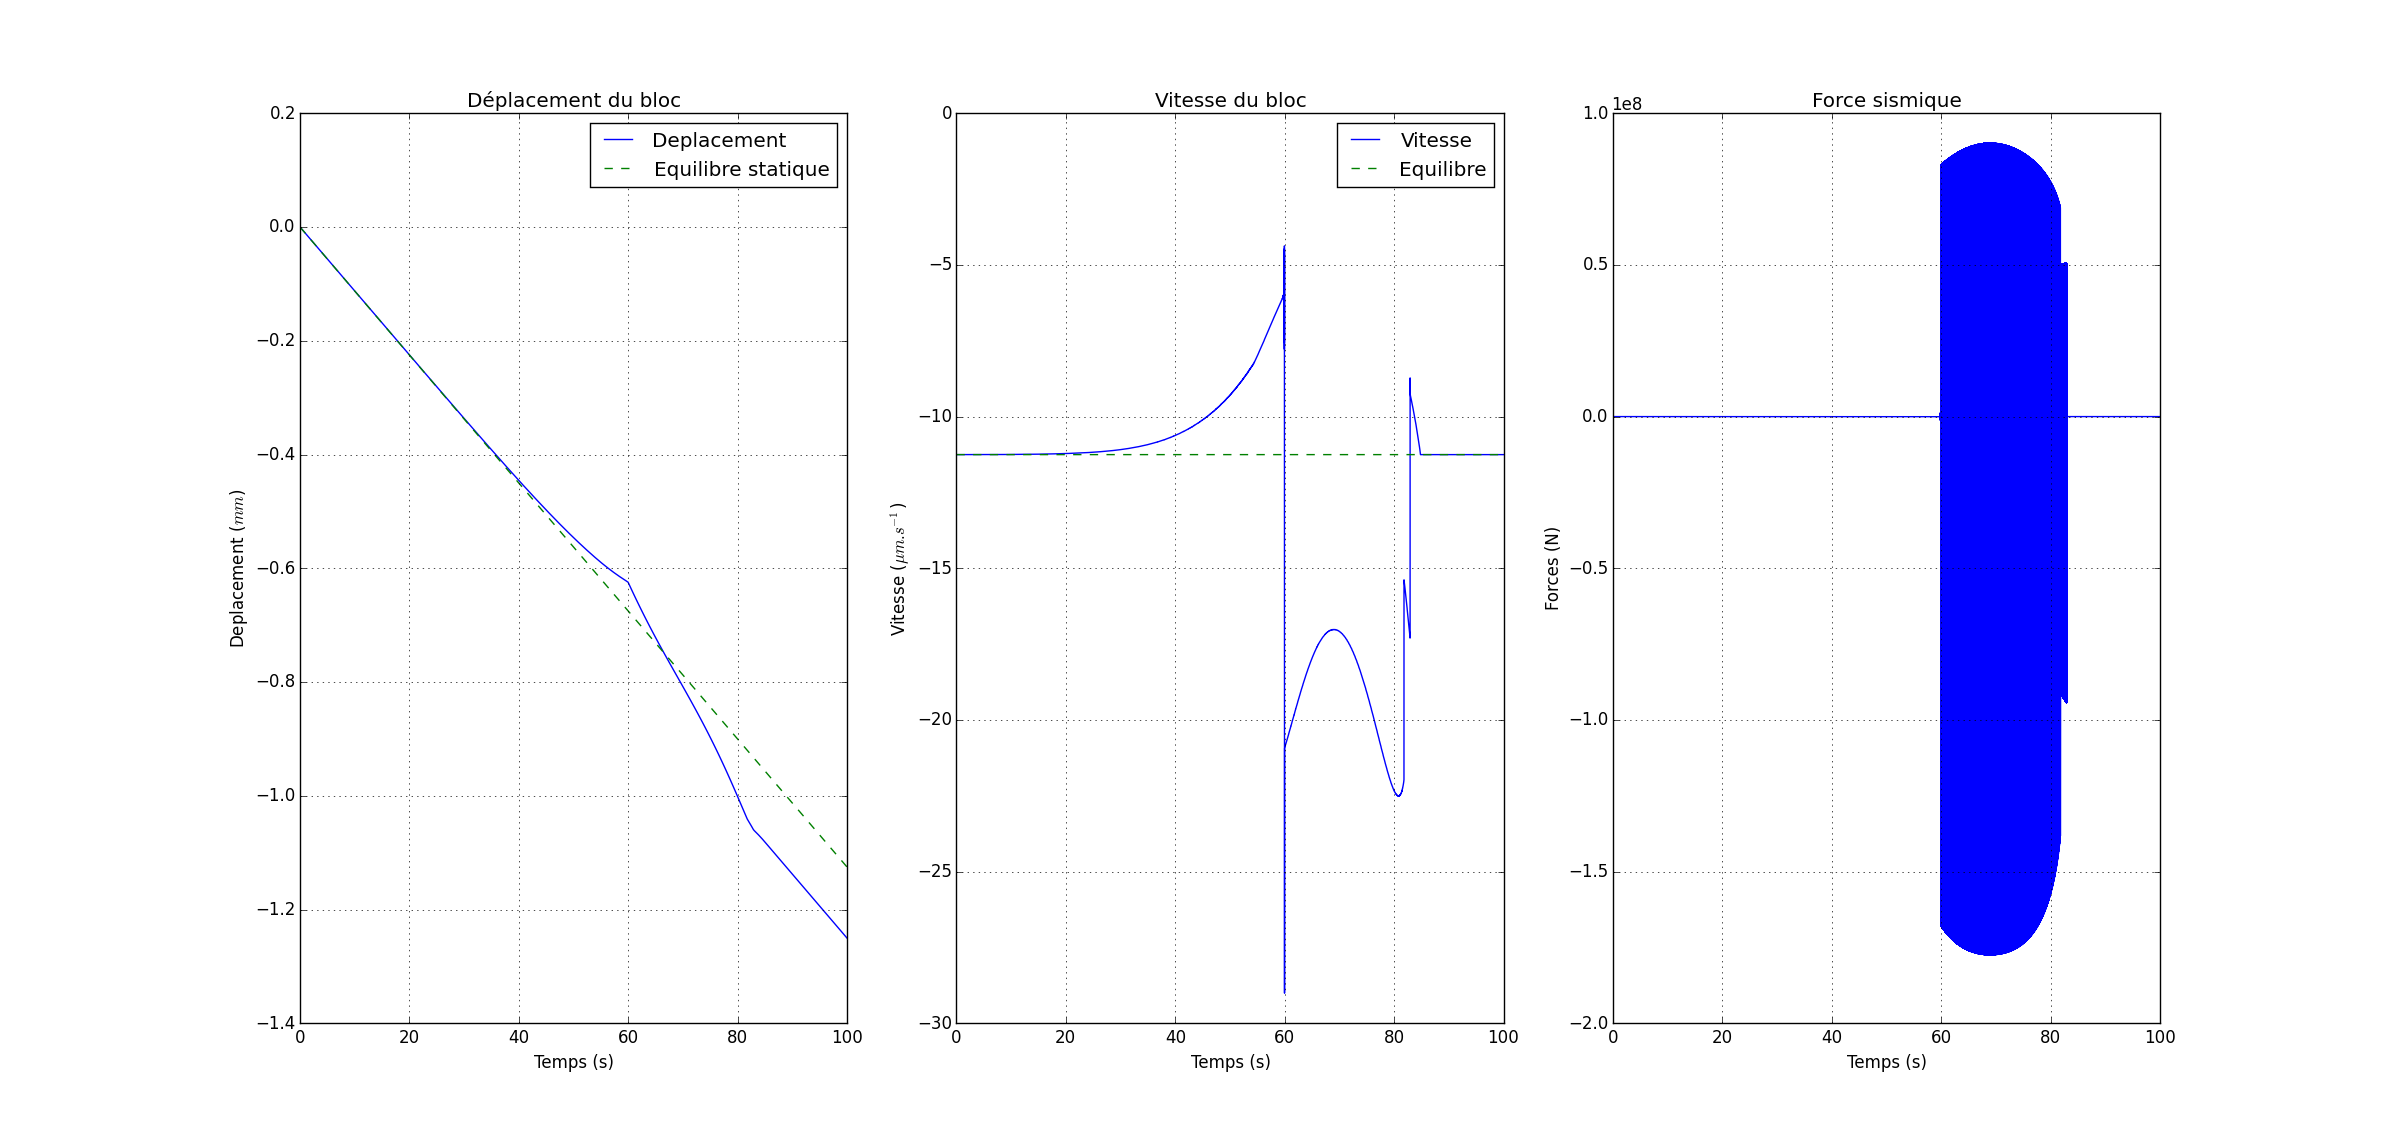
\includegraphics[width=1\linewidth]{figures/Part3/Subpart3/DeplaVitesFsisSubplotInsta.png}
	\label{SubplotDeplaVitesFsisInstaLinear}
	\caption{Figure complète du déplacement, vitesse et force sismique pour $\delta t_{instable}$}
\end{figure}
\underline{Tests dans domaine de stabilité avec $a_1=1$, $ a_2 = 2$, $a_4 = 4$ et $a_8 = 8$} :
\begin{figure}[h!]
	\centering
	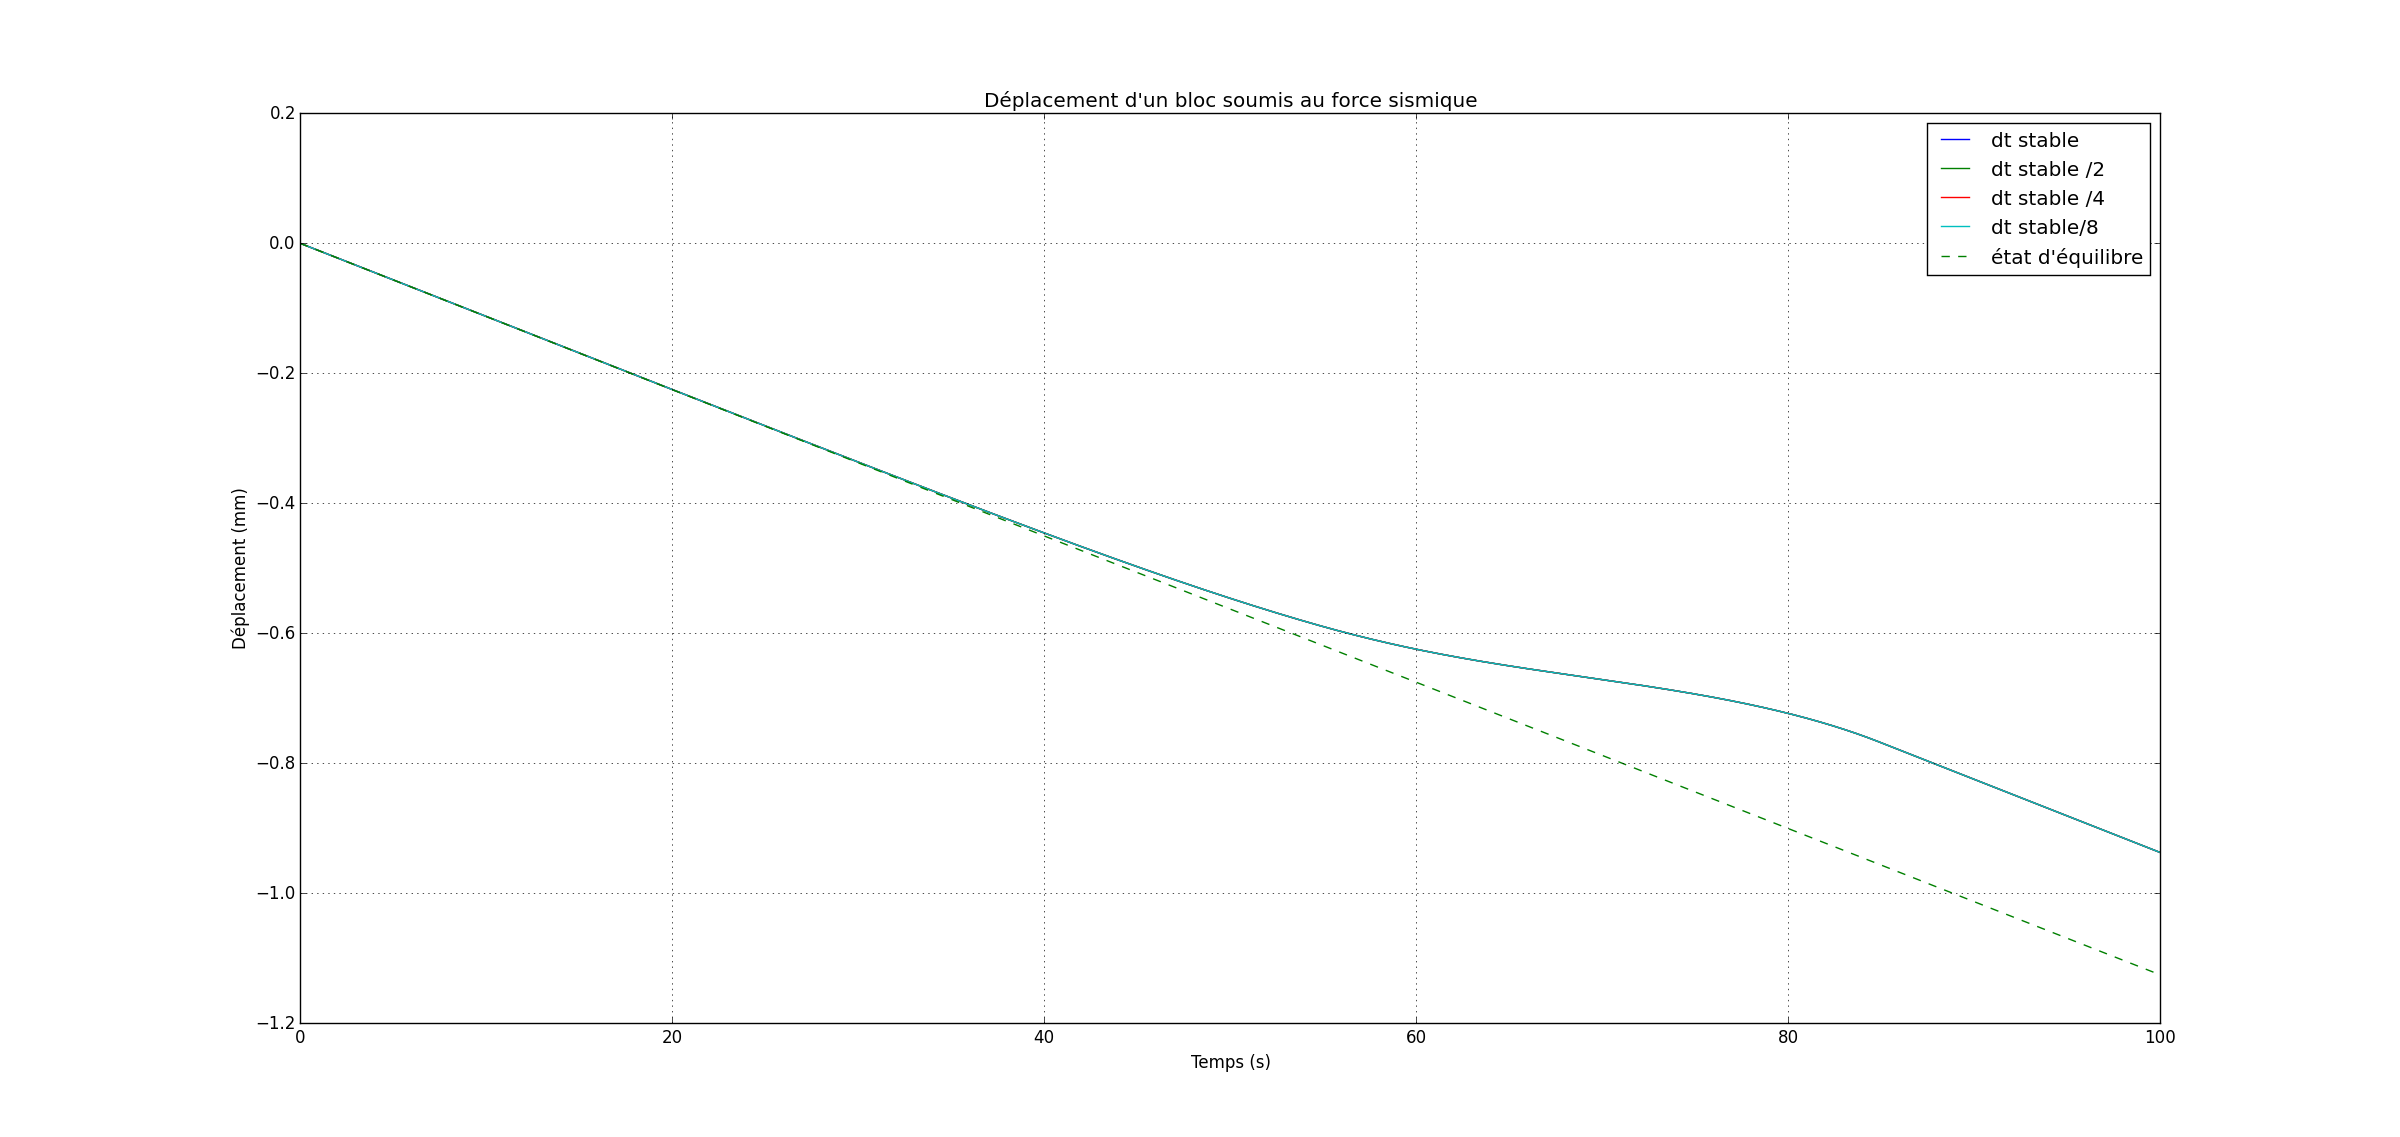
\includegraphics[width=1\linewidth]{figures/Part3/Subpart3/Deplacement.png}
	\caption{Déplacement du bloc au contact de l'iceberg pour différents pas de temps}
	\label{UStableLinear}
\end{figure}

\begin{figure}[h!]
	\centering
	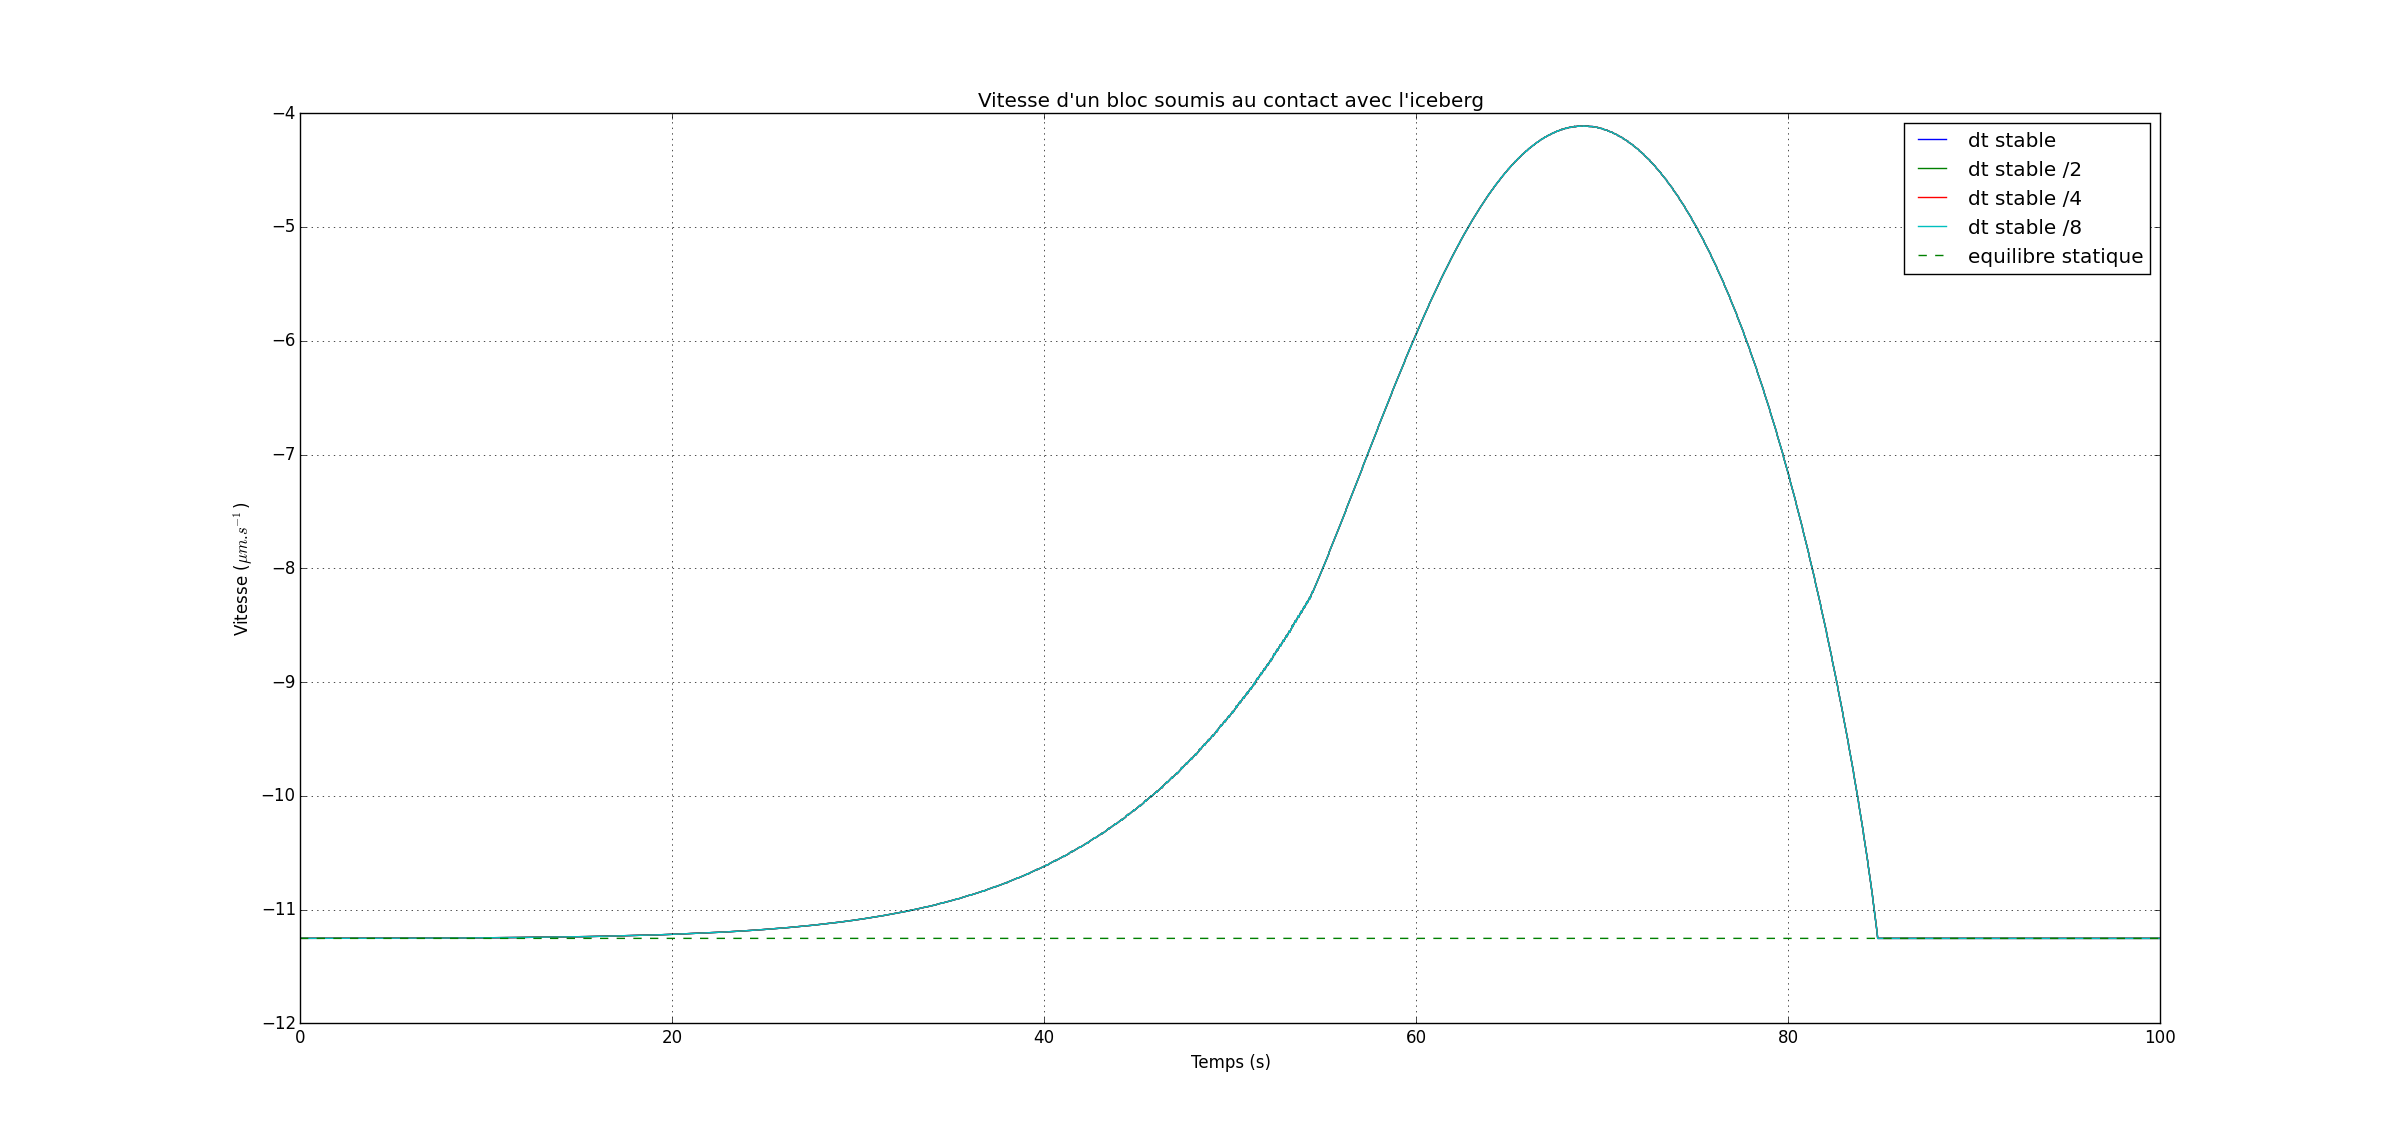
\includegraphics[width=1\linewidth]{figures/Part3/Subpart3/Vitesse.png}
	\caption{Vitesse du bloc au contact de l'iceberg pour différents pas de temps}
	\label{UdStableLinear}
\end{figure}

\begin{figure}[h!]
	\centering
	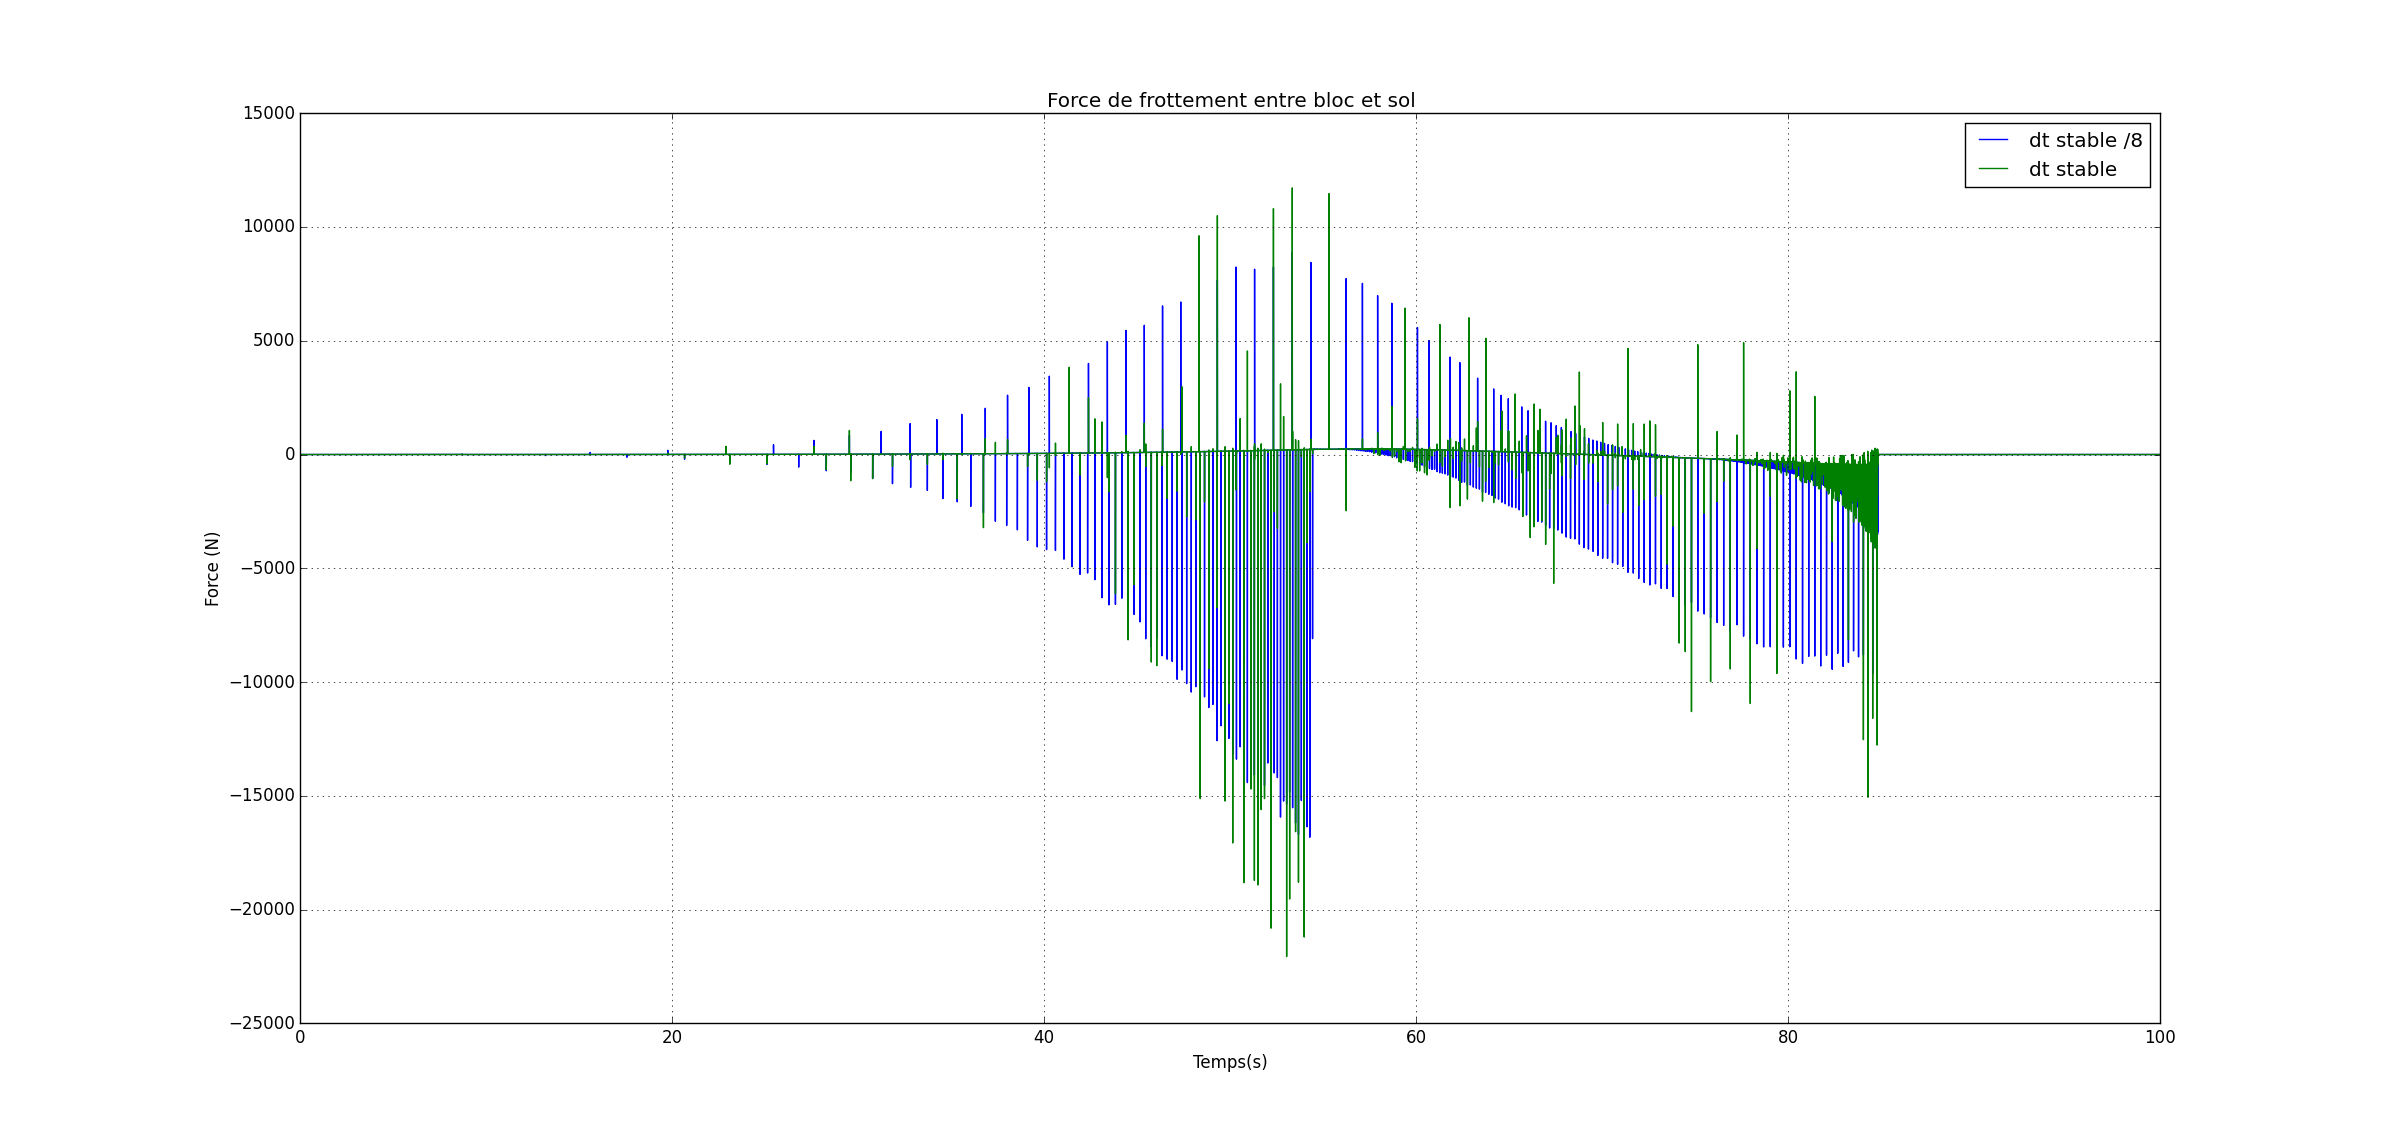
\includegraphics[width=1\linewidth]{figures/Part3/Subpart3/Fsismique.png}
	\caption{Force sismique entre le bloc et le sol au contact de l'iceberg pour différents pas de temps}
	\label{FsisStableLinear}
\end{figure}


\subsection{Formulation du schéma HHT}
Une solution pour régulariser et augmenter la stabilité du schéma numérique serait de changer de schéma numérique. Le schéma de Verlet est purement explicite; passer à un schéma implicite permettrait de régulariser le comportement du glacier en glissement.
\\

Le schéma est paramétré avec une valeur $\alpha$, décrivant le passage du rang $n$ à $n+1$. Le schéma est décrit dans l'article [ajouter le référence de l'article HHT]. Les relations d'état et de passage des variables du rang $n$ à $n+1$ sont décrites dans les équations suivantes.
\\

Les relations \ref{UnHHT}, \ref{UdnHHT} et \ref{UddnHHT} expriment les relations d'état à la première itération du schéma implicite au rang $n$.
\begin{subnumcases}{}
	U_{n+1}^{(1)} = U_n + \delta t \dot{U}_n + \frac{\delta t}{2} \ddot{U}_n \label{UnHHT} \\
	\dot{U}_{n+1}^{(1)} = \dot{U}_n + \delta t \ddot{U}_n \label{UdnHHT} \\
	\ddot{U}_{n+1}^{(1)} = \ddot{U}_{n+1} \label{UddnHHT}
\end{subnumcases}
\\
Pour la suite du calcul, les variables sont itérées. Le rang d'itération est désigné par le paramètre $i$. Dans la pratique, une boucle \textit{While} permet d'itérer les relations suivantes, avec la condition de continuer lorsque que le l'écart entre les vitesses à $i$ et $i+1$ sont supérieures à une certaine erreur.
\\
\begin{subnumcases}{}
	M^* \Delta a^{(i)} = r^{(i)} \label{HHTeqi1} \\
	M^* = M + (1+ \alpha)(\frac{1}{2}-\alpha)\delta t C + (1+\alpha) \frac{1}{4} {(1-\alpha)}^2 \delta t^2 K \label{HHTeqi2} \\
	r^{(i)} = (1+ \alpha)(p_{n+1}-f(U_{n+1}^{(i)},\dot{U}_{n+1}^{(i)}) - \alpha (p_n -f(U_n,\dot{U}_n) - \alpha M^* \Delta a^{(i)} \label{HHTeqi3}
\end{subnumcases}
\\
Grâce à l'équation \ref{HHTeqi1} on trouve notamment le vecteur $\Delta a^{(i)}$ qui permet ensuite de calculer les variables $U_{n+1}^{(i+1)}$, $\dot{U}_{n+1}^{(i+1)}$ et $\ddot{U}_{n+1}^{(i+1)}$ avec respectivement les relations \ref{HHTeqi4}, \ref{HHTeqi5} et \ref{HHTeqi6}. 
\begin{subnumcases}{}
	U_{n+1}^{(i+1)} = U_n^{(i)} + \frac{1}{4} (1-\alpha)^2 {\delta t}^2 \Delta a^{(i)} \label{HHTeqi4} \\
	\dot{U}_{n+1}^{(i+1)} = \dot{U}_n^{(i)} + (\frac{1}{2}-\alpha) \delta t \Delta a^{(i)} \label{HHTeqi5} \\ 
	\ddot{U}_{n+1}^{(i+1)} = \ddot{U}_n^{(i)} + \Delta a^{(i)} \label{HHTeqi6}
\end{subnumcases}
\\
Dans ces equations $M$ désigne la matrice de masse, $C$ la matrice d'amortissement (calculée à partir de la dérivée par rapport à la vitesse), et $K$ la matrice de raideur. Les vecteurs $p$ et $f$ sont respectivement les efforts extérieurs et internes. On note $p_n = p(t_n)$, $p_{n+1} = p(t_{n+1})$ dans la relation \ref{HHTeqi3}. La matrice $M^*$, les vecteurs $r^{(i)}$ et $\Delta a^{(i)}$ sont des variables intermédiaires, propre à l'étape $i$. 
\\ 
Finalement lorsque que l'erreur entre les vitesse $\dot{U}_{n+1}^{(i)}$ et $\dot{U}_{n+1}^{(i+1)}$ devient inférieur à l'erreur souhaité, la boucle s'arrête. Les variables $U_{n+1}$, $\dot{U}_{n+1}$, et $\ddot{U}_{n+1}$ sont définies avec les variables d'état $U_{n+1}^{(i+1)}$, $\dot{U}_{n+1}^{(i+1)}$ et $\ddot{U}_{n+1}^{(i+1)}$. 
\begin{subnumcases}{}
	U_{n+1} = U_{n+1}^{(i+1)} \\
	\dot{U}_{n+1} = \dot{U}_{n+1}^{(i+1)} \\
	\ddot{U}_{n+1} = \ddot{U}_{n+1}^{(i+1)}
\end{subnumcases}
\\

Pour revenir plus précisément au cas du bloc de glacier, les différentes matrices et vecteurs sont tous de longueur et dimension 1, ne sont composées que du terme correspondant au bloc. Le système dynamique est défini avec l'équation \ref{DynaHHT}. Sans effort de liaison élastique, il n'y a pas non plus de matrice de raideur $K$. 
\\
\begin{equation}
	\label{DynaHHT}
	M \ddot{U} + f(U(t), \dot{U}(t)) = p(t)
\end{equation}
Dans l'équation précédente, le vecteur $f$ représente les efforts internes et $p$ les efforts extérieurs. Dans le cas du bloc sans liaisons élastiques. 
\begin{subnumcases}{}
	p(t) = P_{poids \ \mathbf{e_x'} } + F_{perturbation}(t) \label{PHHTexp} \\
	f(t) = -f_{f \ lineaire}(\dot{U}(t)) \label{FHHTexp}
\end{subnumcases}
\\ Les paramètres $C$ et $K$ sont définis à partir de $f$, tels que $C = \frac{\partial f}{\partial \dot{U}}$ et $K = \frac{\partial f}{\partial U}$. $f$ ne dépendant pas du déplacement $U$, $K$ est nul. $C$ dépend de la vitesse et de domaine de linéarité ou non de la force de frottement. 
\begin{equation}
	C = \left\{ \begin{array}{cr}
	\frac{C_W \delta l}{3} (|\dot{U} | )^{-\frac{2}{3}} & \text{si } |\dot{U}| \geq \nu \\
	C_l \delta l & \text{sinon} \end{array} \right . 
	\label{Ceq}
\end{equation}
\\ commentaire sur le facteur C et modifier \ref{HHTeqi2} avec $M^{(i)*}$ 
\subsection{Resultats HHT}
\begin{figure}[h!]
	\centering
	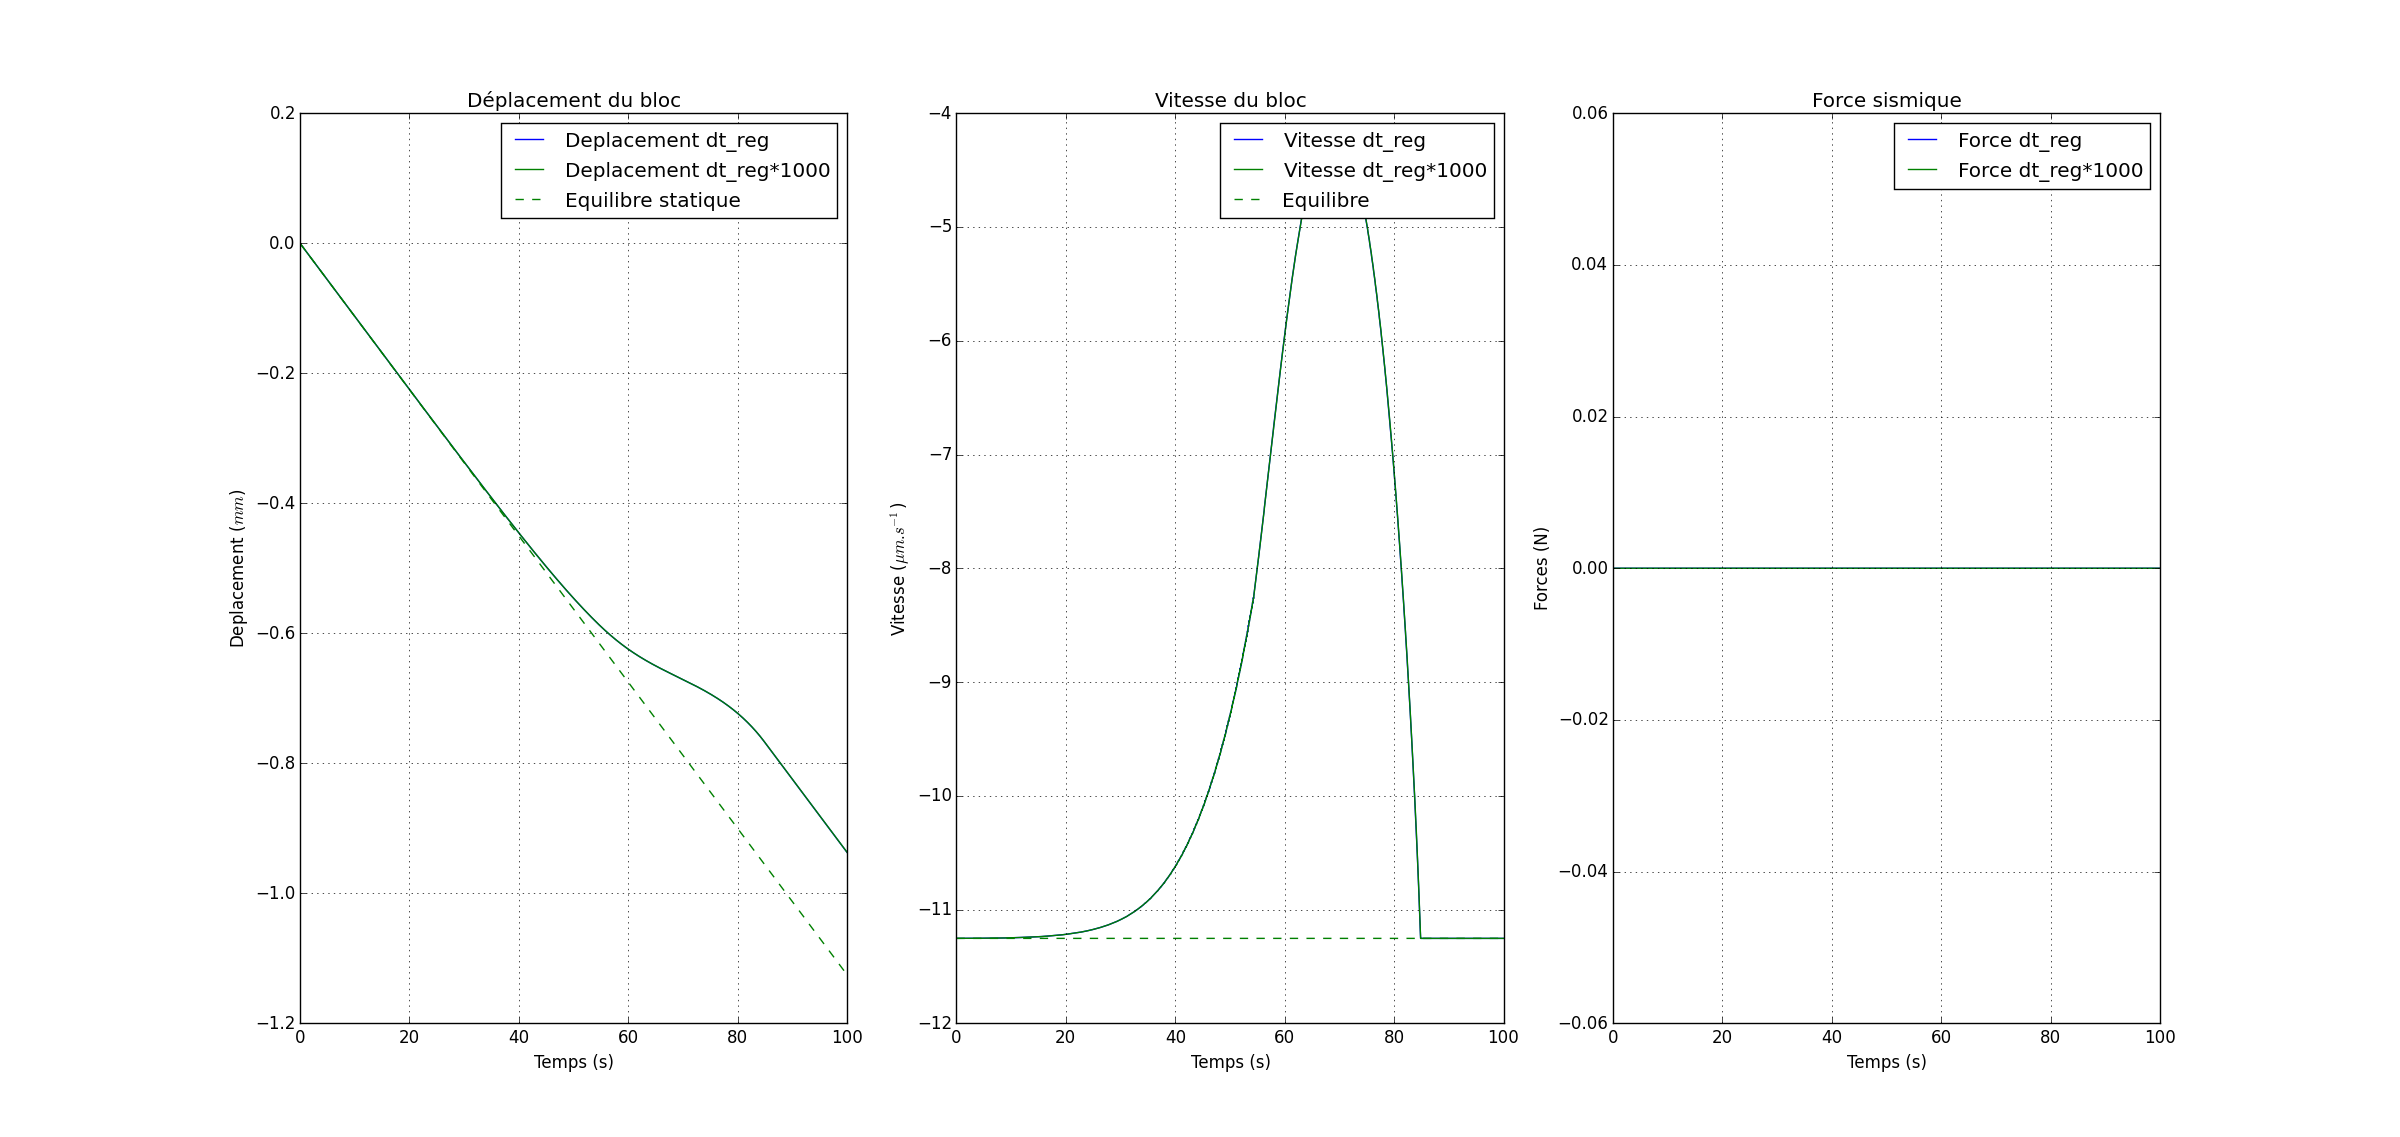
\includegraphics[width=1\linewidth]{figures/Part3/Subpart5/DeplaVitesFsisSubplotStable.png}
	\label{SubplotDeplaVitesFsisStableHHT}
	\caption{Figure complète du déplacement, vitesse et force sismique pour $\delta t_{stable \ lineaire}$ et $1000 \delta t_{stable \ lineaire}$}
\end{figure}

\section{Etude de sensibilité à la taille de bloc}
Dans cette partie on étudie la sensibilité du modèle à la taille des blocs. Le pas de temps sera conservé à $\delta t = 0.0002s$.
\\

On choisis de réduire le longueur du glacier étudié. D'après la figure \ref{MapUtp}, la perturbation se propage sur une longueur dans le glacier. La longueur du glacier est gardée de $2km$. Le modèle est simulé pour différent nombre de bloc. Les tailles de bloc $\delta l$ simulées, et présentées dans les figures suivantes sont de $500m$, $250m$, $100m$, $50m$, $25m$, $10m$ et $5m$. Seuls certains points du glacier seront relevés, ceux calculés avec le modèle le plus grossier. Seuls les points éloignés de $500m$, $1km$, $1.5km$ et $2km$, et au front du glacier seront affichés.
\\

La figure \ref{UmaxDlLoop} présente la variation du maximum du déplacement perturbé à différent éloignement du terminus du glacier. L'amplitude de perturbation varie en effet en fonction de la taille des éléments. Celle-ci dépend plus de la taille d'élément au front du glacier. Le déplacement semble converger vers une valeur au front du glacier. La convergence est plus difficile pour les points plus proches du front du glacier.
\\

\begin{figure}[h!]
	\centering
	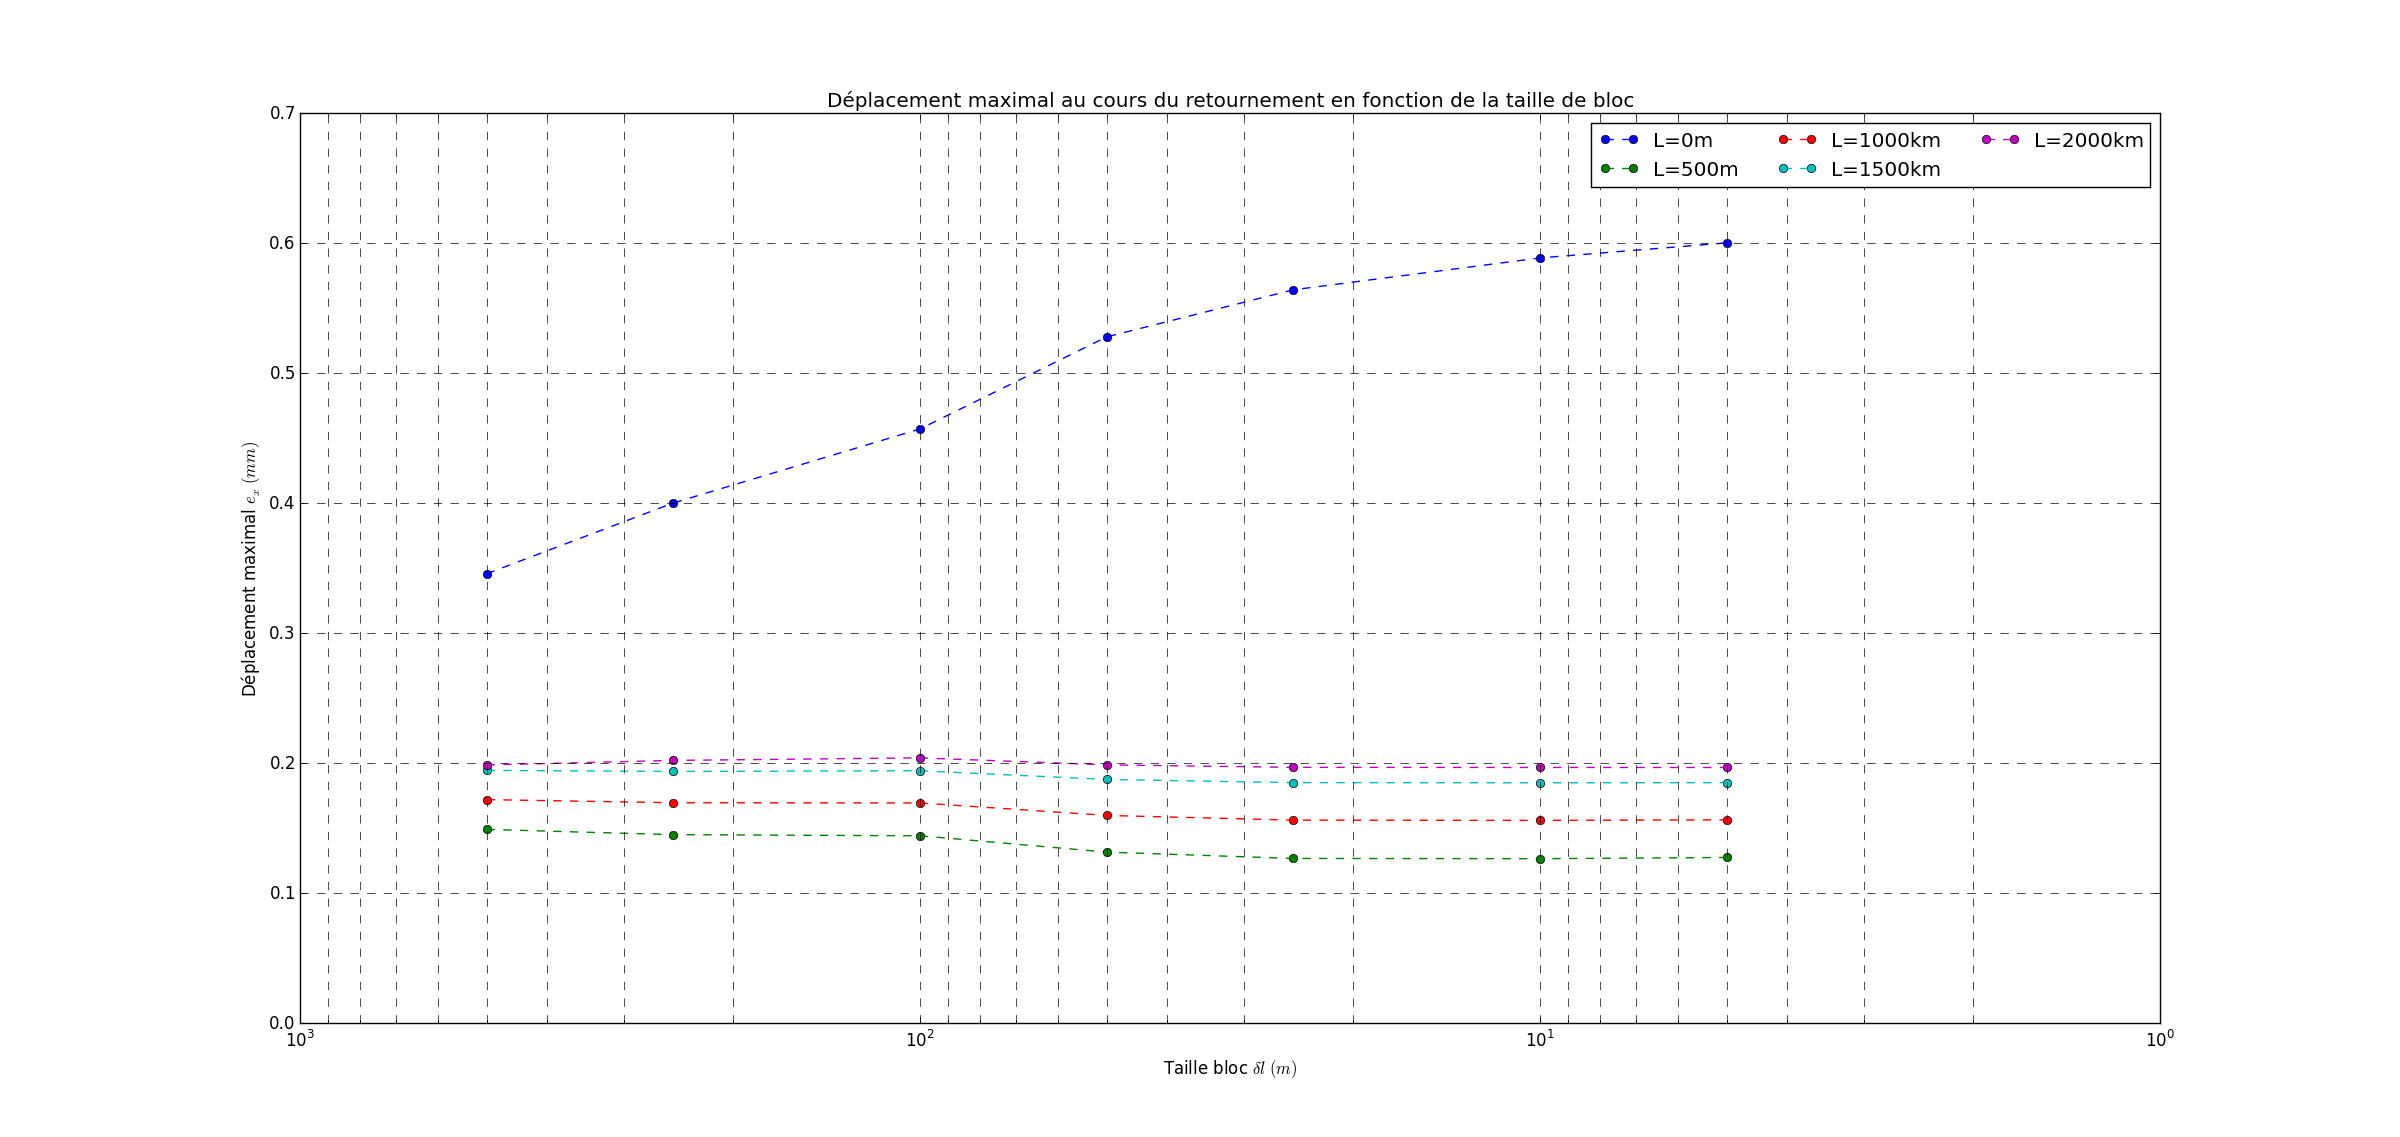
\includegraphics[width=1\linewidth]{figures/Part4/Displacement.png}
	\caption{Amplitude du déplacement en fonction de la taille de bloc}
    \label{UmaxDlLoop}
\end{figure}
De même, la figure \ref{UdmaxDlLoop} présente l'évolution de l'amplitude de la vitesse à différent point en fonction de la taille des blocs. La vitesse ne varie pas de la même façon que le déplacement perturbé en fonction de la taille d'élément. Toutefois la convergence reste plus difficile au front du glacier. Celle des autres blocs est en revanche plus rapide que la convergence du déplacement.
\\ A travers ces deux figures on remarque pas de problème d'instabilité comme avec le pas de temps $\delta t$. En effet, l'expression de \ref{DtStableEq} ne dépend pas de $\delta l$, et $\delta t$ reste inférieur à la limite de stabilité qui est induite par les efforts de liaison élastique ($\delta t_{stable \ élastique} = 0.025s$ pour $\delta l= 25m$ la limite la plus faible). On reste donc au dessus de celle-ci.
\\

\begin{figure}[h!]
	\centering
	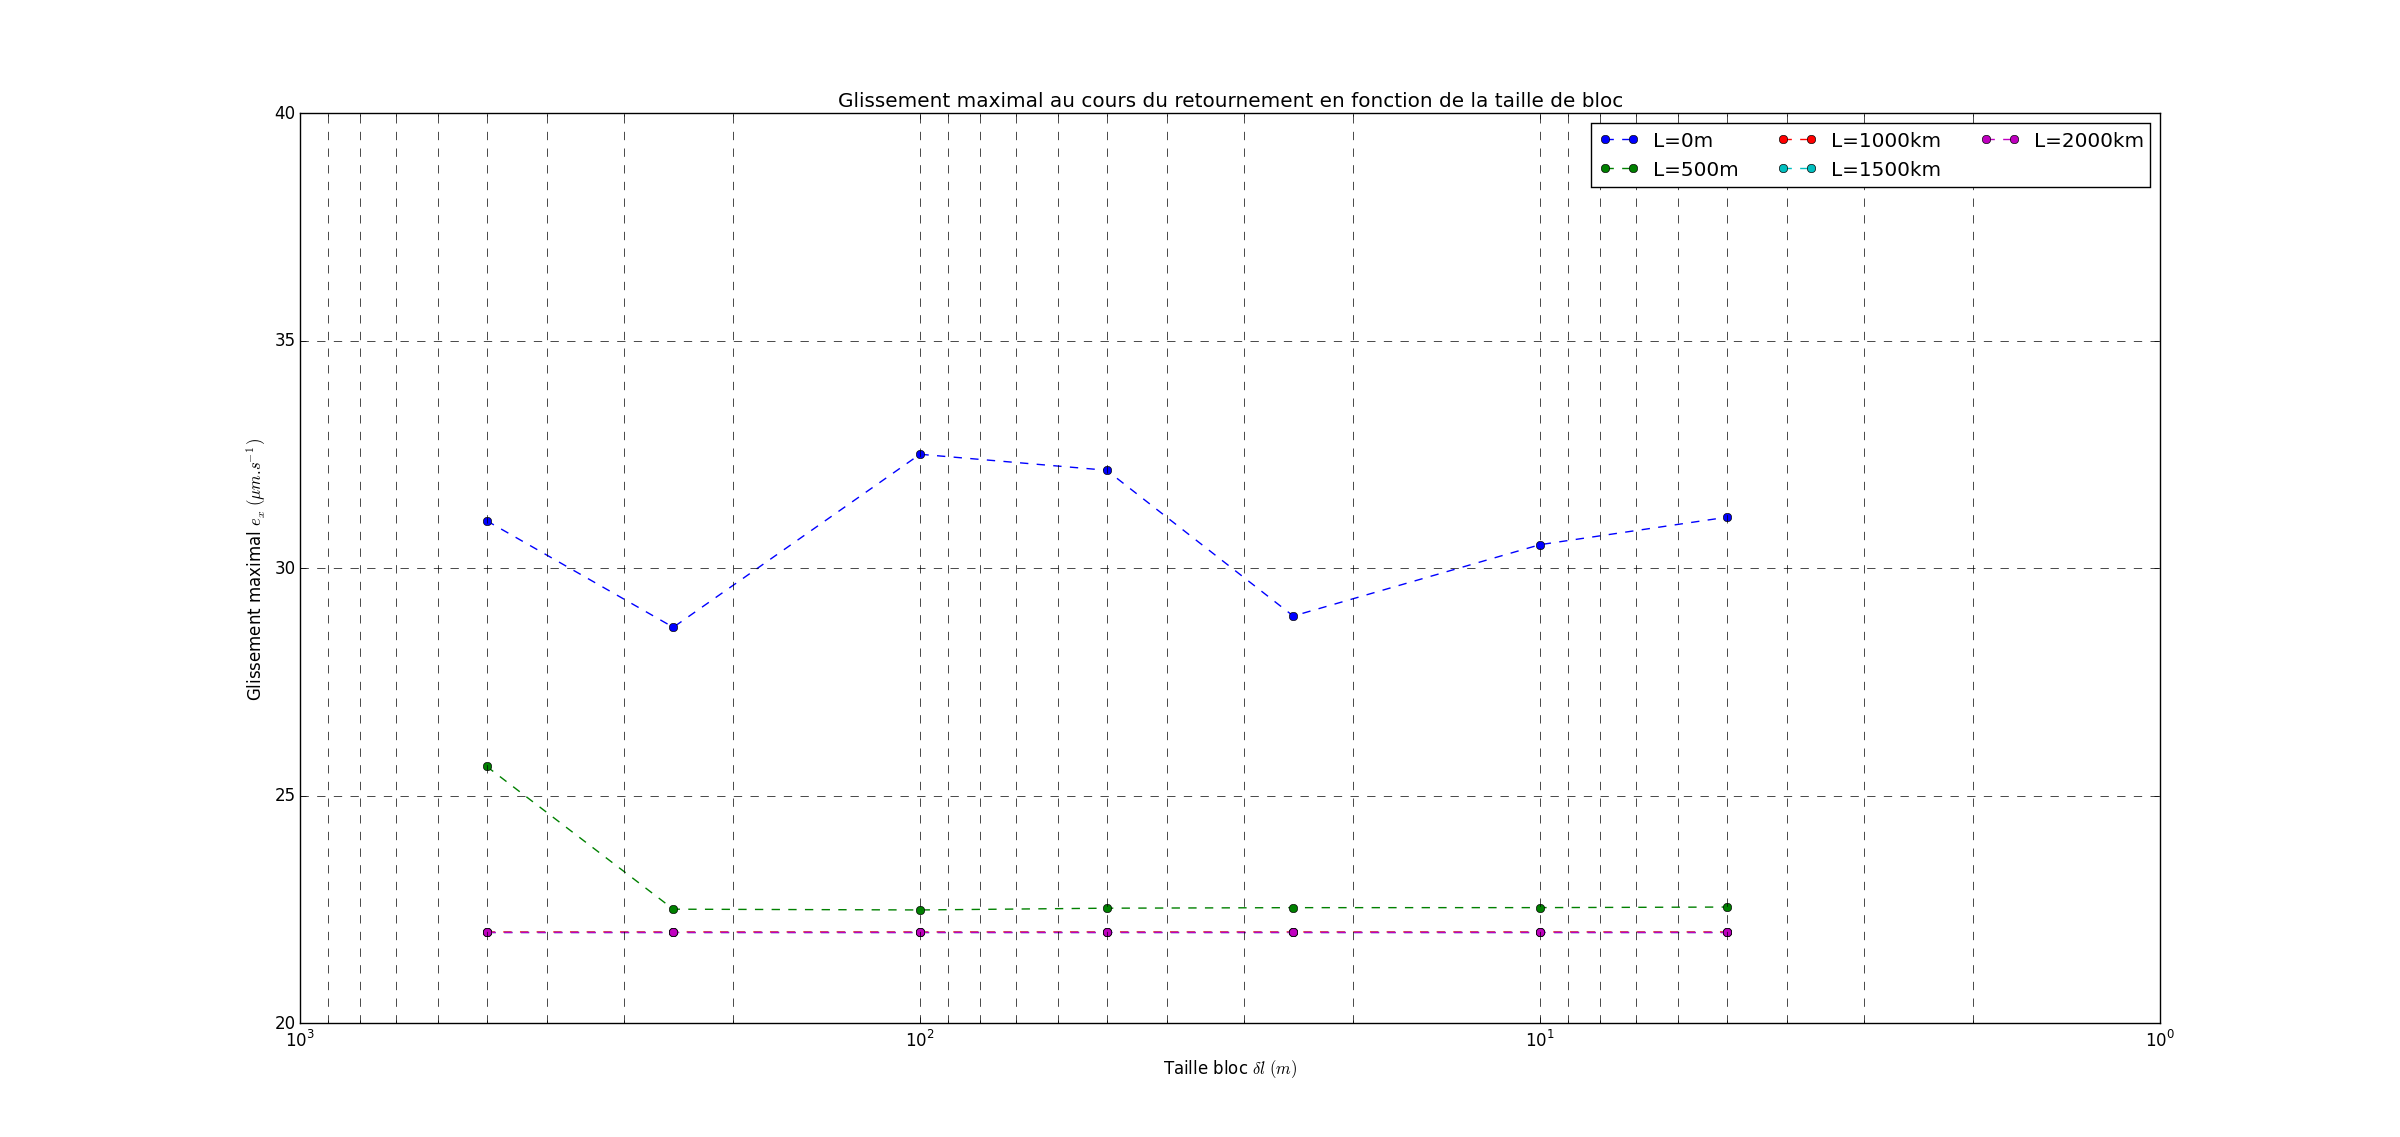
\includegraphics[width=1\linewidth]{figures/Part4/SpeedSlide.png}
	\caption{Amplitude de la vitesse en fonction de la taille de bloc}
    \label{UdmaxDlLoop}
\end{figure}
La figure \ref{FcontactDlLoop} présente l'évolution de l'amplitude de la force sismique en fonction de la taille des blocs. Contrairement aux deux figures précédentes, la force sismique semble moins sensible à la taille des blocs, et converge plus rapidement. Sa convergence plus rapide est héritée de celle cumulé de tout les blocs. Le manque de convergence en vitesse au front du glacier (car la force de frottement dépend uniquement de la vitesse aux blocs à paramètres fixés) ne semble pas avoir trop d'effet sur celle de la force sismique. On remarque qu'à partir de $\delta l = 25m$, la force sismique a convergé. On trouve en faite $F_{sismique}(\delta l =25m) = 310.7499\ GN.m^{-1}$ et $F_{sismique}(\delta l = 5m) = 310.7505\ GN.m^{-1}$, $\delta l = 25 m$ permet d'obtenir une valeur proche à $99.99 \%$ de celle trouvée avec $\delta l = 5 m$.
\\

\begin{figure}[h!]
	\centering
	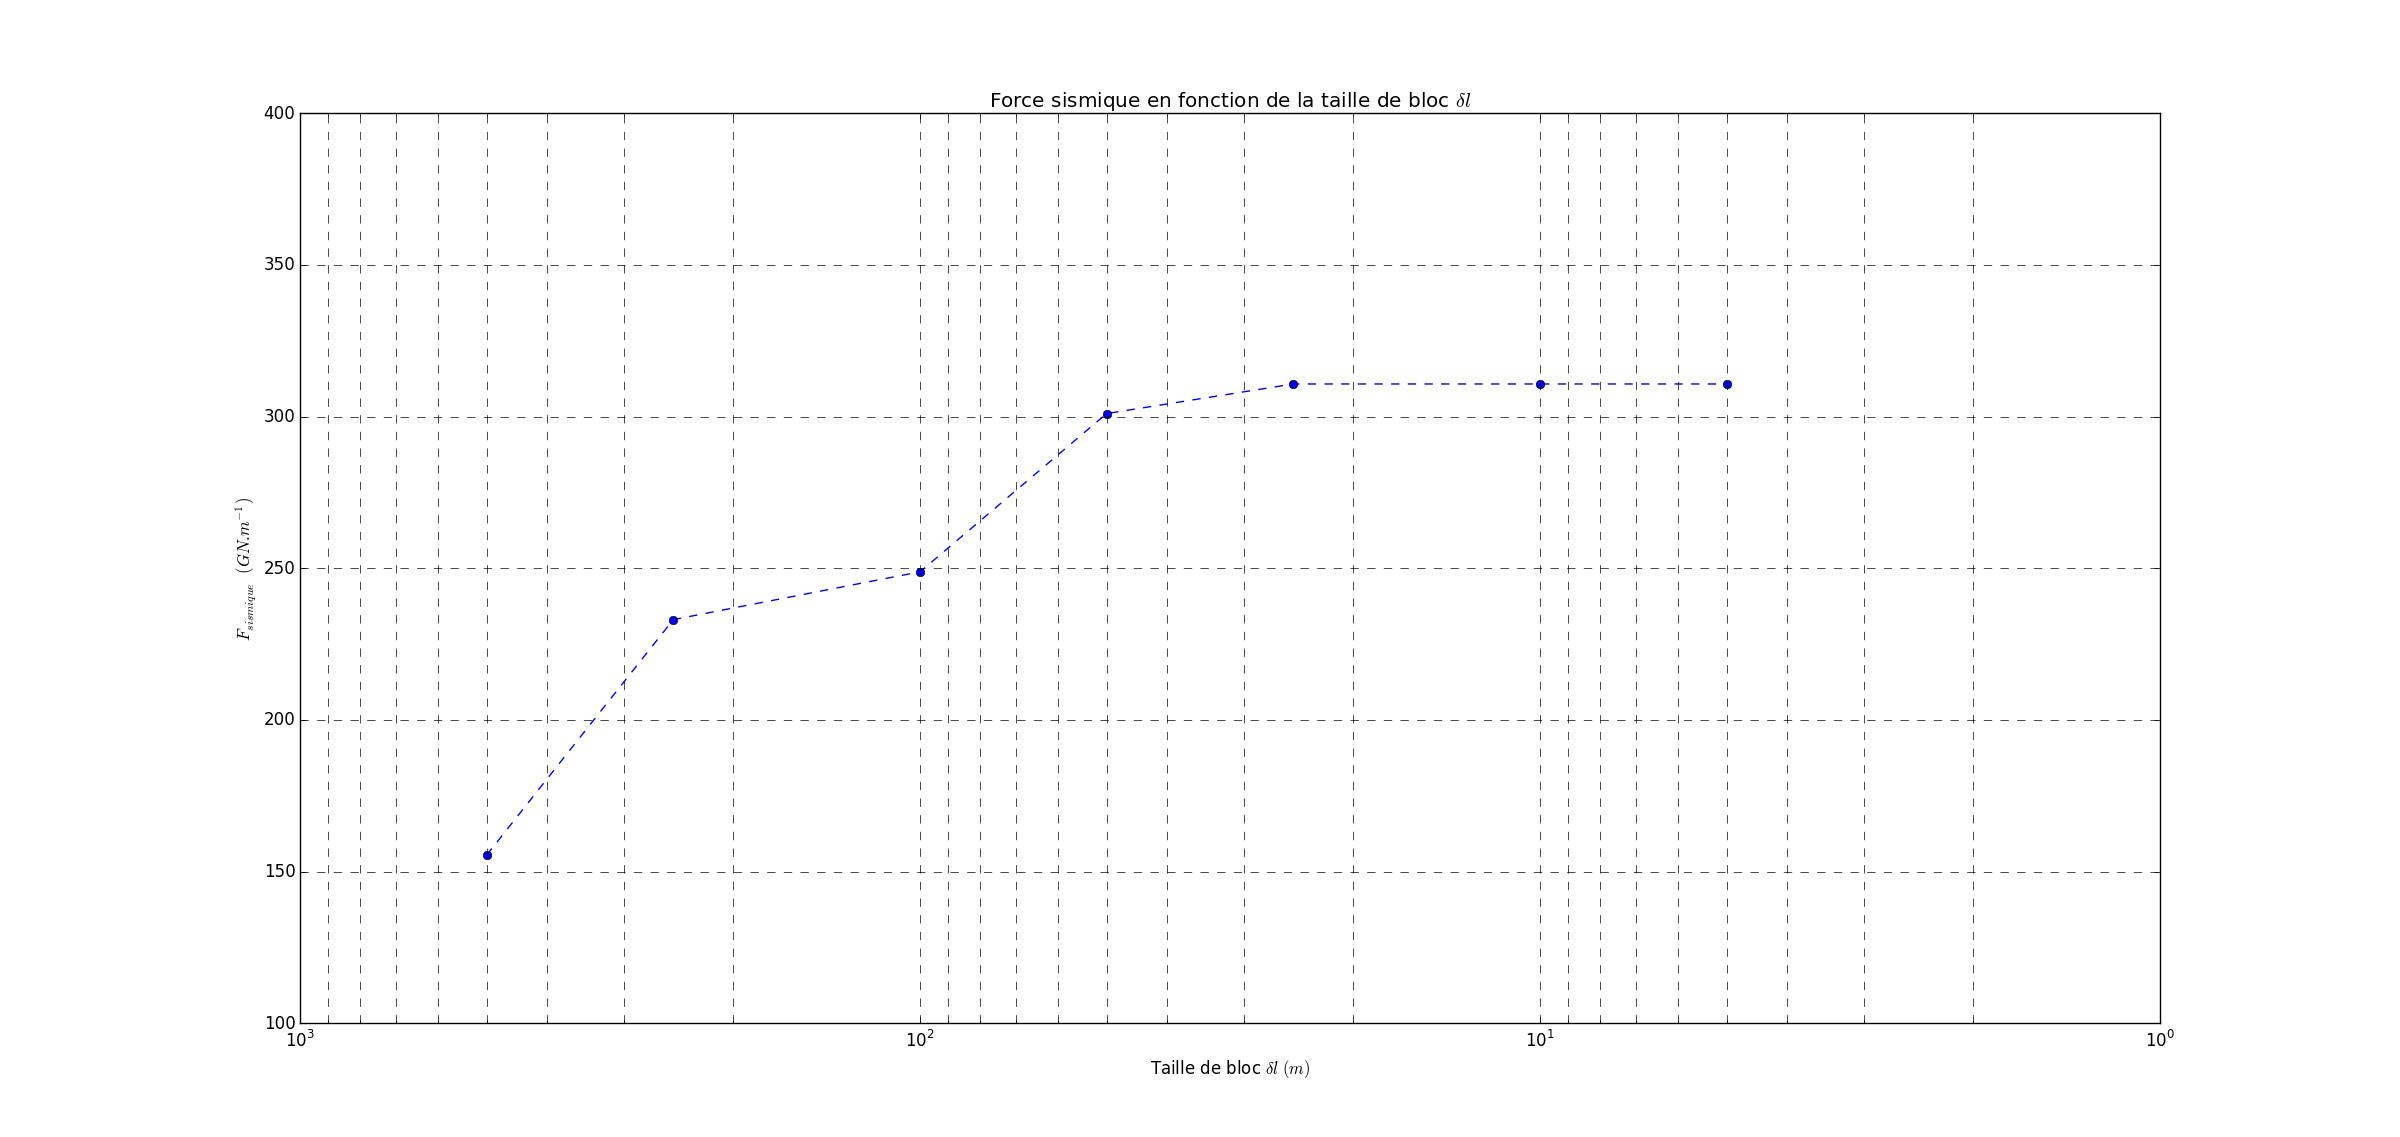
\includegraphics[width=1\linewidth]{figures/Part4/Fsismique.png}
	\caption{Amplitude de la force de contact en fonction de la taille de bloc}
    \label{FcontactDlLoop}
\end{figure}
Enfin la figure \ref{TpsComputeDlLoop} montre la temps de calcul en fonction de la taille des éléments. Il dépend de la puissance de calcul et de l'écriture du programme. Le programme n'est pas optimisé en mémoire, les valeurs à chaque blocs sont conservées. 
\\ On peut remarquer que le temps de la calcul du modèle dépend plus de la taille, ou de la dimension des variables à chaque itération que du nombre d'itération. En effet contrairement à la figure \ref{TpsComputeDtLoop} montrant une évolution linéairement du temps de calcul en fonction de $N_t$, la courbe figure \ref{TpsComputeDlLoop} augmente non-linéairement en fonction du nombre de bloc. Une réduction du nombre de bloc sera plus important que celle de pas de temps.
\\

\begin{figure}[h!]
	\centering
	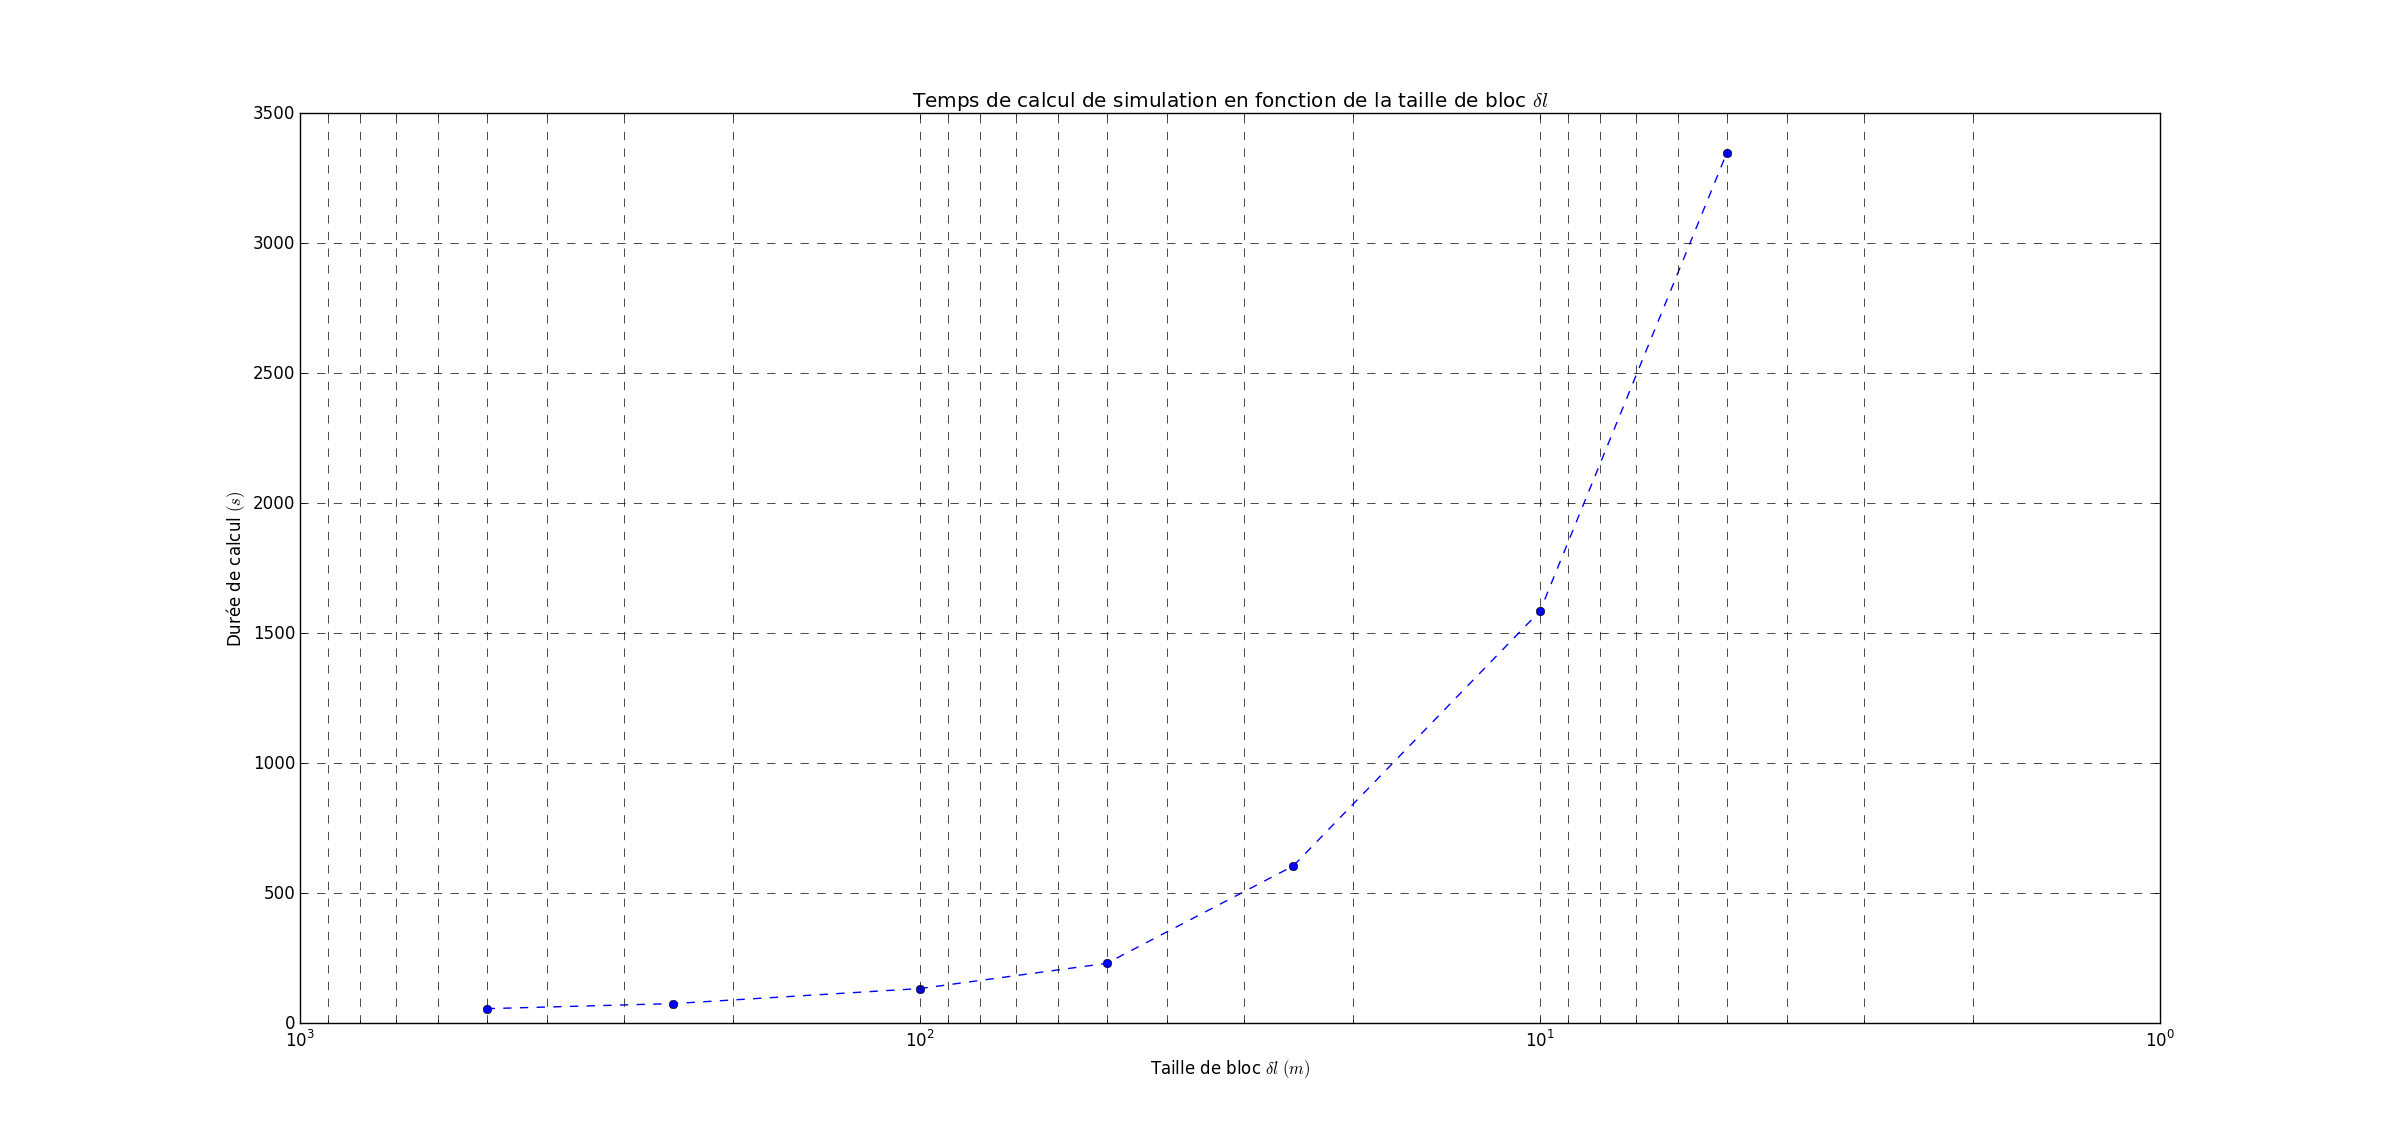
\includegraphics[width=1\linewidth]{figures/Part4/TpsCompute.png}
	\label{TpsComputeDlLoop}
\end{figure}
\section{Comparaison de stabilité avec schéma Hilbert-Hughes-Taylor}
Dans cette partie nous nous intéressons à la stabilité du modèle de Verlet avec celle employant le schéma de Hilbert-Hughes-Taylor (HHT) présenté dans l'article \cite{Hughes1989}. Le schéma est paramétré avec un $\alpha$. Seul le schéma en $\alpha$ est considéré. 
\setlength{\parindent}{1cm} Le schéma utilise les formules suivantes \ref{VecteursDetat} à chaque itération pour calculer le déplacement ($U_{n+1}$), la vitesse ($\dot{U}_{n+1}$) et l'accélération ($\ddot{U}_{n+1}$) au rang $n+1$. 
\\

Les equations d'état au premier rang:
\begin{subnumcases}{}
	U_{n+1}^{(1)} = U_n + \delta t \dot{U}_n + \frac{1}{2} \delta t^{2} \ddot{U}_n  \label{VecteursDetat1}\\
	\dot{U}_{n+1}^{(1)} = \dot{U}_n + \delta t \ddot{U}_n \label{VecteursDetat2} \\
	\ddot{U}_{n+1}^{(1)} = \ddot{U}_n \label{VecteursDetat3}
\end{subnumcases}
\setlength{\parindent}{1cm} Dans un second temps, un nouvel équilibre est cherché avec une boucle jusqu'à convergence ($i$ désigne le rang de cette boucle). Les forces extérieures $p_n$ et $p_{n+1}$ aux instants $t_n$ et $t_{n+1}$. Cette force désigne la force de contact de l'iceberg. Ces relations d'équilibre font également intervenir les efforts internes $f_n$ et $f_{n+1}$ qui dépendent des vecteurs déplacement et vitesse du système. 
\begin{subnumcases}{}
	M^{*} \Delta \ddot{U}^{(i)} = r^{(i)} \label{HHTeq1} \\
	M^{*} = M + (1+\alpha)(\frac{1}{2} - \alpha) \delta t C + (1+\alpha) \frac{1}{4} (1-\alpha)^2 K \label{HHTeq2} \\
	\Delta \ddot{U}^{(i)} = (1+\alpha) p_{n+1} - \alpha p_n -M \ddot{U}_{n+1}^{(i)} - (1+\alpha) f_{n+1} + \alpha f_n \label{HHTeq3}
\end{subnumcases}
\\

La relation \ref{HHTeq2} fait intervenir les matrices $K$ d'élasticité et $C$ d'amortissement. Ces deux matrices sont définies telles que $K = \frac{\partial f}{\partial U}$ et $C = \frac{\partial f}{\partial \dot{U} }$. La matrice d'amortissement est calculée en prenant une vitesse $\dot{U}$ proche de $\dot{U}_{eq}$ et en considérant la loi de Weertman comme loi de frottement. Après linéarisation, on déduit que la matrice d'amortissement s'exprime telle que :

\begin{equation}
C= \frac{1}{3} sign(\dot{U}_{eq}) \delta l C_W |\dot{u}_{eq} |^{-\frac{2}{3}} \begin{pmatrix} 
\frac{1}{2} & 0 & \cdots & \cdots & 0 	   \\
0           & 1 & 		 & 		  & \vdots \\
\vdots 		&   & \ddots &        & \vdots \\
\vdots  	&   &        & 1      & 0      \\
 0          & \cdots & \cdots & 0 & \frac{1}{2}
 \end{pmatrix} \label{CmatrixEq}
\end{equation}
\\

La variation de l'accélération $\Delta \ddot{U}^{(i)}$ permet ensuite d'itérer les vecteurs déplacement, de vitesse et d'accélération, données par les expressions suivantes:
\begin{subnumcases}{}
	U_{n+1}^{(i+1)} = U_n^{(1)} + \frac{1}{4}(1-\alpha)^2 \delta t^2 \Delta \ddot{U}^{(i)} \label{VecteurUn11} \\
	\dot{U}_{n+1}^{(i+1)} = \dot{U}_n^{(i)} + (\frac{1}{2} - \alpha) \delta t \Delta \ddot{U}^{(i)} \label{VecteurUn12} \\
	\ddot{U}_{n+1}^{(i+1)} = \ddot{U}_{n+1}^{(i)} + \Delta \ddot{U}^{(i)} \label{VecteurUn13}
\end{subnumcases}
\setlength{\parindent}{1cm} Lorsque la boucle à converger en position vitesse et accélération, l'équilibre au pas de temps $t_{n+1}$ est considéré atteint. Le schéma défini le déplacement, la vitesse et l'accélération à l'instant $t_{n+1}$ tels que $U_{n+1} = U_{n+1}^{(i+1)}$, $\dot{U}_{n+1} = \dot{U}_{n+1}^{(i+1)}$ et $\ddot{U}_{n+1} = \ddot{U}_{n+1}^{(i+1)}$. 
\\

Dans l'étude de la stabilité, on considère tout d'abord un chargement extérieur nul à tout instant tel que $\forall n, \quad p_n = {0}$. On considère seulement une faible varaition de vitesse autour de la vitesse d'équilibre du système. On suppose que le schéma est stable si le déplacement perturbé , la vitesse et l'accélération restent nulles. L'équilibre pour chaque instant calcul $t_n$ doit être atteint à la première itération tel que $U_{n+1} = U_{n+1}^{(2)}$, $\dot{U}_{n+1} = \dot{U}_{n+1}^{(2)}$ et $\ddot{U}_{n+1} = \ddot{U}_{n+1}^{(2)}$ avec $i=1$. En linéarisant la force de frottement et en simplifiant le terme de frottement à la vitesse d'équilibre avec le poids tangentiel, l'expression \ref{HHTeq3} devient:
$$ \Delta \ddot{U}^{(1)} = - M \ddot{U}_{n+1}^{(1)} -(1+\alpha) \left( K U^{(1)} + C \dot{U}^{(1)} \right) + \alpha \left( K U_{n} + C \dot{U}_{n} \right) $$
\\ On exprime facilement les vecteurs $U^{(1)}$, $\dot{U}^{(1)}$ et $\ddot{U}^{(1)}$ en fonction de $U_n$, $\dot{U}_n$ et $\ddot{U}_n$ grâce aux expressions \ref{VecteursDetat1}, \ref{VecteursDetat2} et \ref{VecteursDetat3}.
\\ On déduit finalement l'expression schéma associé au vecteur $q_n = \begin{Bmatrix} U_n \\ \dot{U}_n \\ \ddot{U}_n \end{Bmatrix}$. 
\\ On définie dans l'expression \ la matrice $R$ qui permet de reformuler l'expression \ref{HHTeq1} en fonction de $[M^*]^{-1}$ et $q_n$. 
\begin{align*}
	\Delta \ddot{U}^{(1)} &= [M^*]^{-1} [R] q_n \\
	\text{avec} \quad [R] &= \begin{bmatrix} -[K] & - \left( [C] + (1+\alpha)\delta t [K] \right) & -\left( [M] + (1+\alpha) \delta t [C] + (1+\alpha) \frac{\delta t^2}{2} [K]  \right) \end{bmatrix}
\end{align*}
\\

Pour passer à l'expression du vecteur $q_{n+1}$, on définie la matrice $[\Gamma ] $ qui permet d'exprimer les termes de variation additionner au vecteur $q_n$, grâce aux expressions \ref{VecteurUn11}, \ref{VecteurUn12} et \ref{VecteurUn13}. La matrice d'amplification est notée $[\Lambda]$.
\begin{align*}
q_{n+1} &= q_n + [\Gamma] \Delta \ddot{U}^{(1)} \\
\quad &= \left( I_{3 (N_p+1)} + [\Gamma] [M^*]^{-1} [R] \right) q_n \\
\quad &= [ \Lambda ] q_n
\end{align*}
$$ \text{avec} \quad [\Gamma] = \begin{bmatrix}  (1-\alpha)^2 \frac{\delta t^2}{4} I_{N_p+1} \\ (\frac{1}{2} - \alpha) \delta t I_{N_p+1} \\ I_{N_p+1} \end{bmatrix} $$
Finalement on retient l'expression de la matrice d'amplification:
\begin{equation}
[\Lambda] = I_{3 (N_p+1)} + [\Gamma] [M^*]^{-1} [R] \label{LambdaMatrix}
\end{equation}
\\

Pour étudier le stabilité du schéma, on étudie les valeurs propres de la matrice d'amplification du système, plus particulièrement son rayon spectral. Le rayon spectral de la matrice $[\Lambda ]$ doit avoir un rayon inférieur ou égal à 1, tel que $\rho(\Lambda) <1$. On concervera pour les différents calculs les paramètres géométriques du glacier suivants $N_p = 50$, $L_{tot} = 5km$ et $\delta l = 100m$, assurant une bonne convergence d'après la partie précédente.
\setlength{\parindent}{1cm} La figure \ref{MapRhoHHT} présente la carte du rayon spectral en fonction de $\delta t $ (avec un balayage logarithmique entre $\delta t_{max}=1s$ et $\delta t_{min}=10^{-6}s$) et du paramètre $\alpha$. L'article \cite{Hughe1989} annonce que le paramètre $\alpha$ habituel pris varie entre 0 et $-\frac{1}{3} $. 
\\

Cette figures permet de donner une allure de la dépendance en $\alpha$. La limite de stabilité ne semble pas dépendre de $\alpha$. En revanche la figure présente également la dépendance en $\delta t$, le pas de temps. La limite semble atteinte quelque soit $\alpha$ pour la même valeur de $\delta t$, d'environ $ \mathbf{\delta t_{stable} = 4.10^{-5}s }$. Cette limite est inférieur à $\delta t_{stable} = 4.10^{-4}s$ imposée par le schéma de Verlet.
\begin{figure}
	\centering
	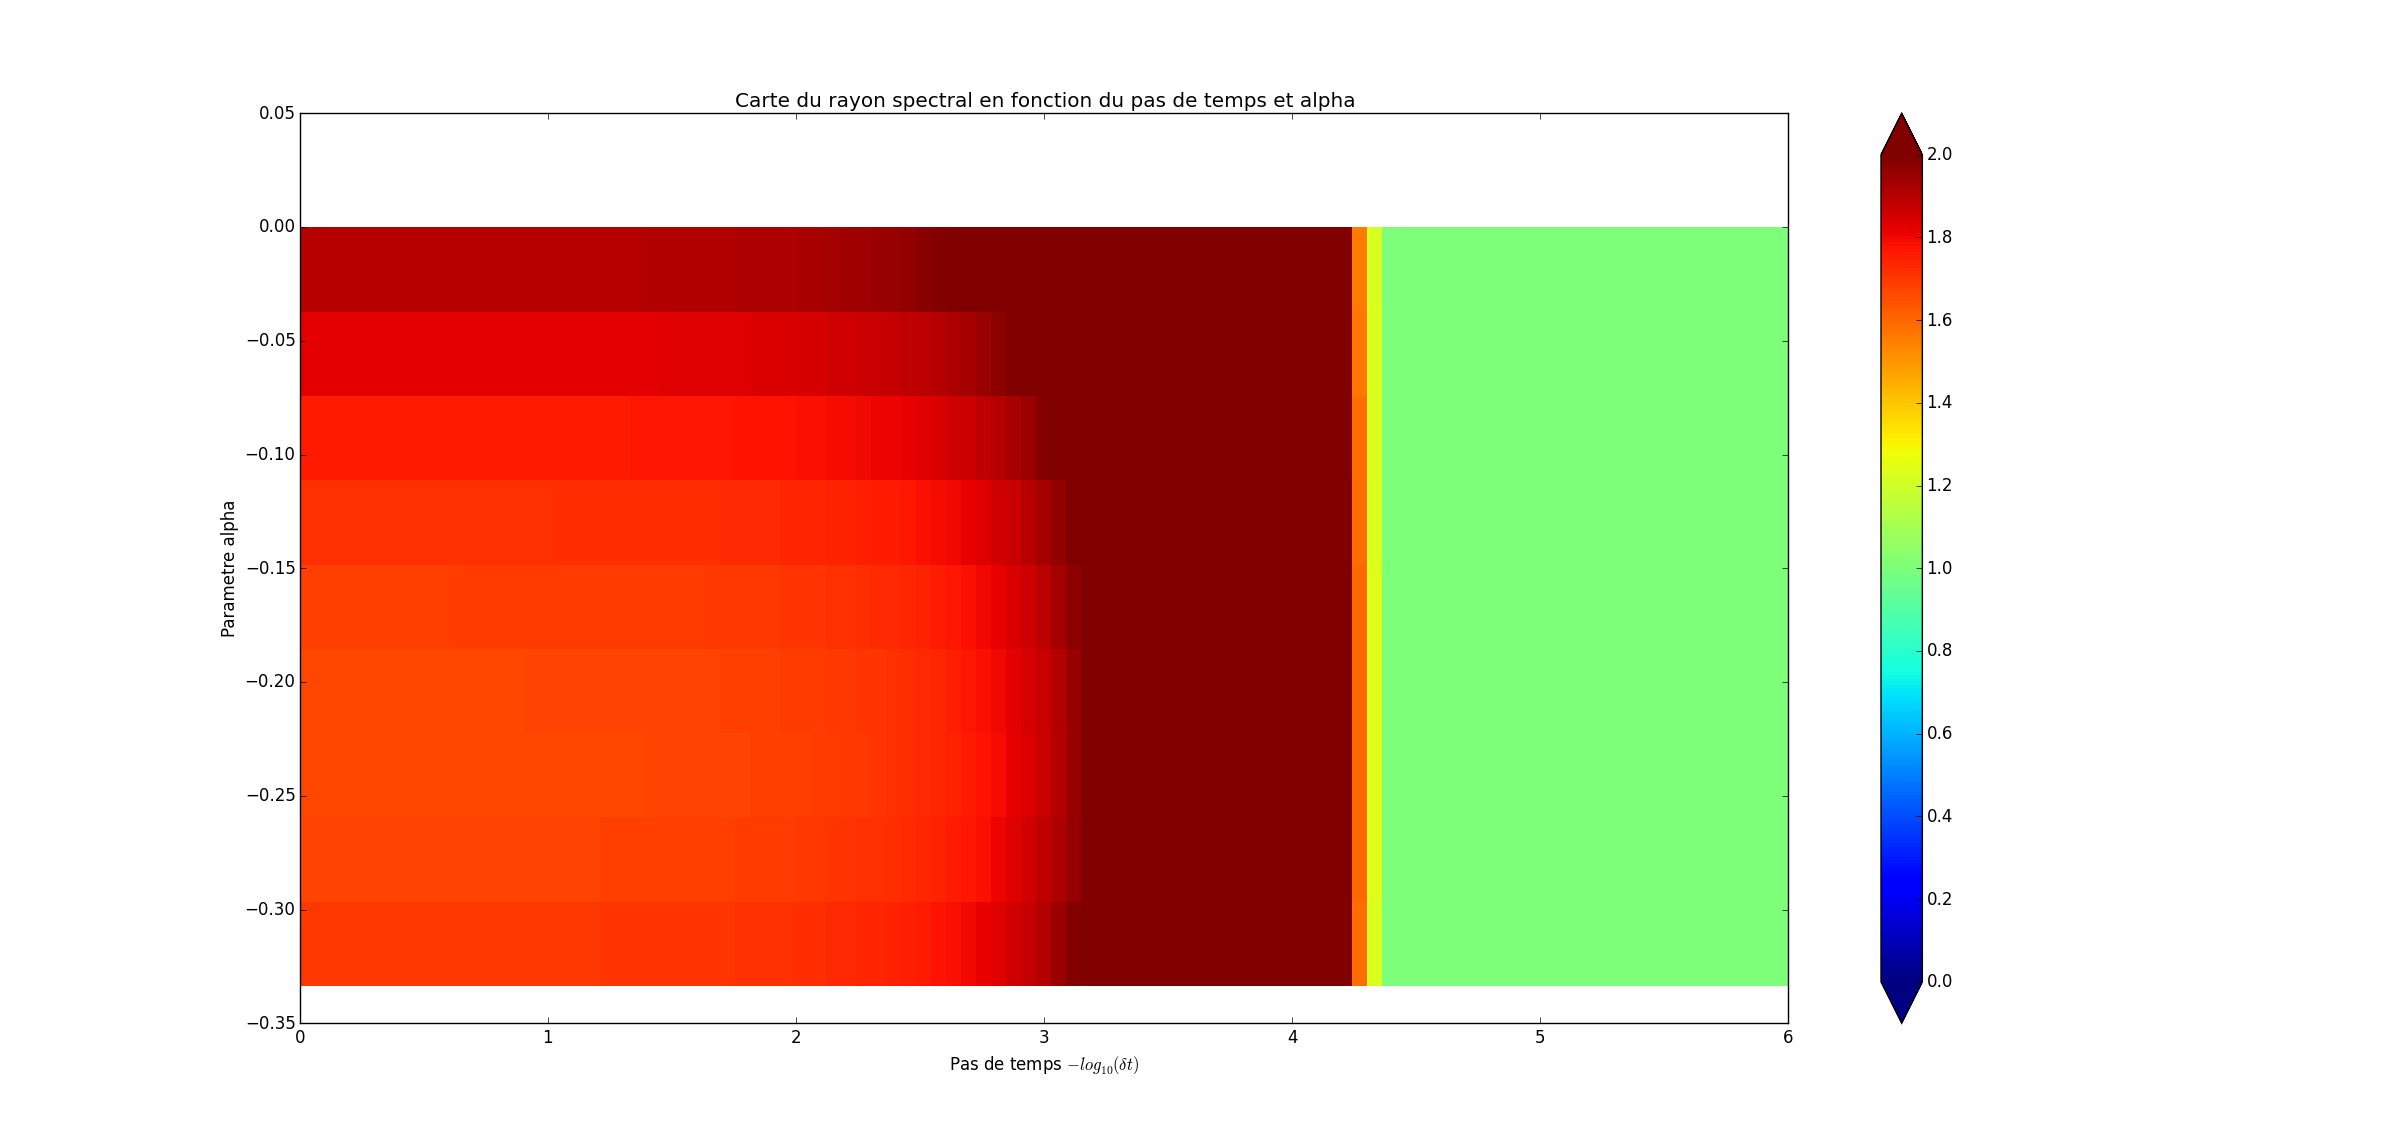
\includegraphics[width=1\linewidth]{figures/Part5/MapRhoHHT.png}
	\label{MapRhoHHT}
	\caption{Carte du rayon spectral avec $-log_{10}(\delta t)$ en abscisse et $\alpha$ en ordonné}
\end{figure}
\\

La figure \ref{RhoHHT} relève mieux la limite de stabilité du schéma en fonction du pas de temps $\delta t$. Plusieurs courbes sont affichées pour différentes valeurs de $\alpha$. La limite de stabilité semble rester la même pour ces différentes valeurs, conservant toujours le même $\delta t_{stable}$. 
\begin{figure}
	\centering
	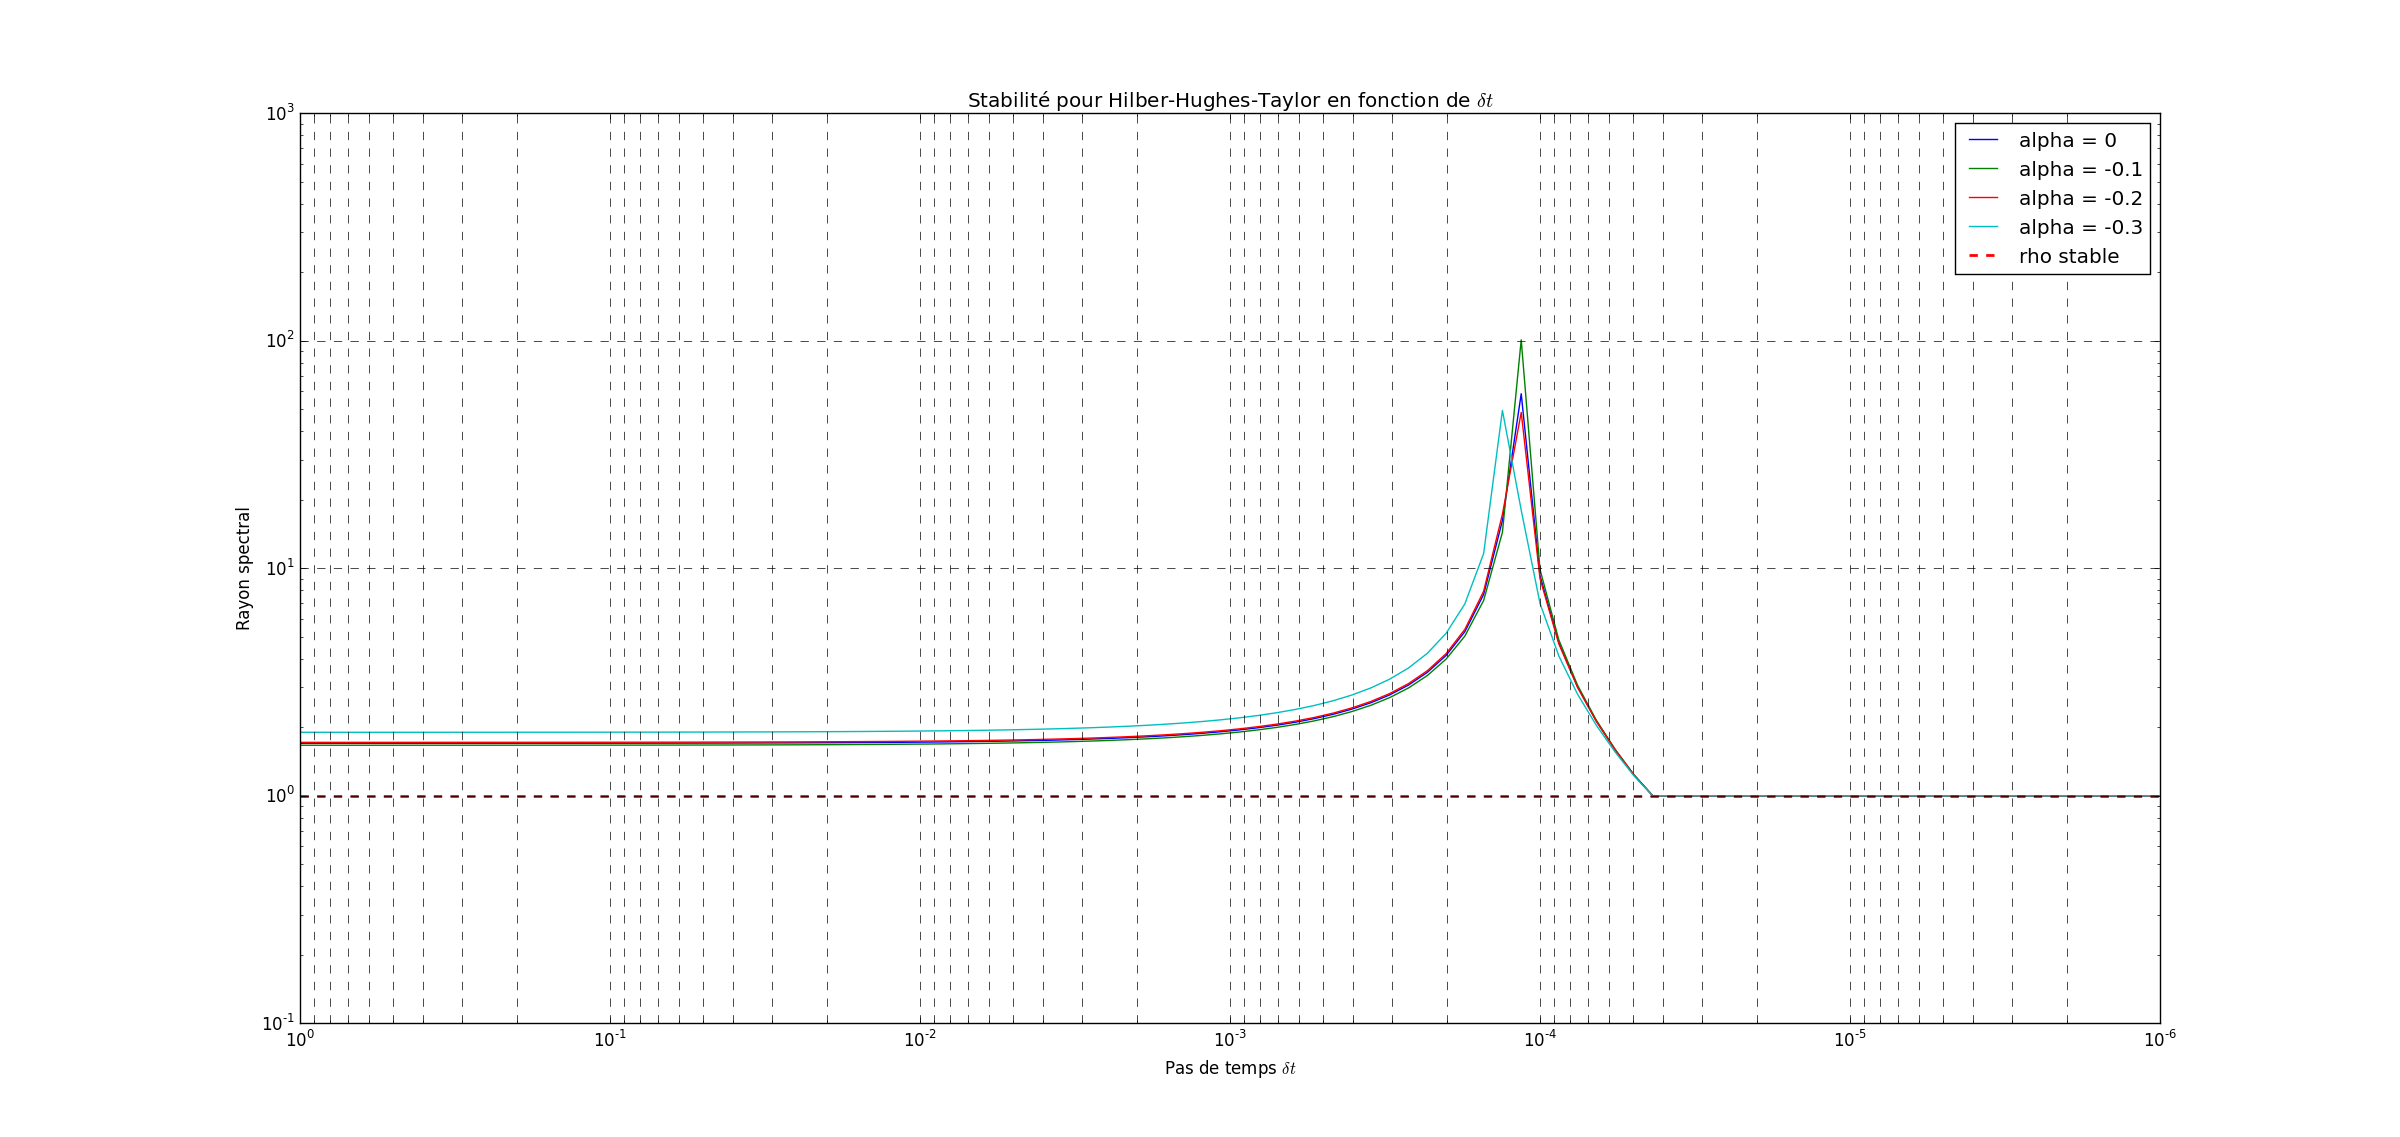
\includegraphics[width=1\linewidth]{figures/Part5/RhoHHT.png}
	\label{RhoHHT}
	\caption{Détails du rayon spectral en fonction du pas de temps $\delta t$}
\end{figure}
\\

Pour comparer ces valeurs de rayons spectrales et la précision de ce critère, on cherche également le rayon spectral pour le schéma de Verlet. En reprenant les formules \ref{UiEq}, \ref{Fn1Eq} et \ref{UdiEq}, dans le cas statique sans la force de perturbation, on cherche la matrice d'amplification correspondante.
\\

Pour l'expression de cette de matrice, on exprime tout d'abord la force de frottement $F_f$ sous forme linéarisée en fonction de la vitesse de perturbation $\left\{ \dot{U}_{n \ p} \right\}$. On rajoute également la force élastique de liaison $F_e$. On pas $n+1$, la résultante des forces s'exprime en fonction de $\left\{ U_{n+1} \right\}$ déplacement au rand $n+1$ calculé à partir de l'équation \ref{Un1Eq}, et de la vitesse au rang $n$  $\left\{ \dot{U}_n \right\}$.
$$ F_{n+1} = F_e(U_{n+1}) + F_f(\dot{U}_n)$$
En utilisant l'expression de la matrice C (\ref{CmatrixEq}) et K, on a finalement :
\begin{equation}
	F_{n+1} = [K] \left\{ U_{n+1} \right\} + [C] \left\{ \dot{U}_n \right\} 
	\label{Fn1Eq2}
\end{equation}
En reprenant le système d'équation \ref{UiEq}, \ref{Fn1Eq} et \ref{UdiEq}, et en définissant le vecteur d'intérêt $\left\{ q_n \right\} = \begin{Bmatrix} U_n \\ F_n \\ \dot{U}_n \end{Bmatrix} $. La matrice d'amplification s'exprime entre les vecteurs $\left\{ q_n \right\}$ et $\left\{ q_{n+1} \right\}$. On trouve le système suivant:
\begin{equation}
	\begin{bmatrix} I_{N_p +1 } & 0 & 0 \\ -[K]&I_{N_p +1}& 0 \\ 0 & -\frac{\delta t}{2} [M]^{-1} & I_{Np +1}\end{bmatrix} \begin{Bmatrix} U_{n+1} \\ F_{n+1} \\ \dot{U}_{n+1} \end{Bmatrix} = \begin{bmatrix} I_{N_p +1 } & \frac{\delta t^2}{2} [M]^{-1} & \delta t I_{N_p +1} \\ 0 &0 & [C] \\ 0 & \frac{\delta t}{2} [M]^{-1} & I_{Np +1}\end{bmatrix} \begin{Bmatrix} U_{n} \\ F_{n} \\ \dot{U}_{n} \end{Bmatrix} 
	\label{SysVerletEq}
\end{equation}
On remarque dans cette expression que la force $F_{n+1}$ au rang $n+1$ ne dépendant pas $F_n$. Le terme centrale de la matrice de droite dans \ref{SysVerletEq} est nul. 
\\ On définit la matrice d'amplification $[A]_{Verlet}$ entre les vecteurs $\left\{ q_n \right\}$ et $\left\{ q_{n+1} \right\}$ d'après l'expression suivante \ref{AmatrixVerletEq}.
\begin{equation}
	\left\{ q_{n+1} \right\} = [A]_{Verlet} \left\{ q_n \right\} 
	\label{AmatrixVerletEq}
\end{equation}
On en conclut grâce à la relation précédente \ref{AmatrixVerletEq} et au système matriciel \ref{SysVerletEq}, la matrice d'amplification pour le schéma de Verlet s'exprime tel que présenté avec la relation \ref{AmatrixVerletExp}. On remarque que la matrice de gauche dans le système \ref{SysVerletEq} est bien inversible car diagonale supérieure avec uniquement des 1 sur sa diagonale. 
\begin{equation}
	[A]_{Verlet} = \begin{bmatrix} I_{N_p +1 } & 0 & 0 \\ -[K]&I_{N_p +1}& 0 \\ 0 & -\frac{\delta t}{2} [M]^{-1} & I_{Np +1}\end{bmatrix}^{-1} \begin{bmatrix} I_{N_p +1 } & \frac{\delta t^2}{2} [M]^{-1} & \delta t I_{N_p +1} \\ 0 &0 & [C] \\ 0 & \frac{\delta t}{2} [M]^{-1} & I_{Np +1}\end{bmatrix} 
	\label{AmatrixVerletExp}
\end{equation}
\\

A titre de comparaison, on peut également construire le schéma de Verlet du système sans le contact de l'iceberg en négligeant les forces de frottement. On supprime la dépendance en $\dot{U}_n$ dans l'expression de $F_{n+1}$ dans \ref{Fn1Eq2}, et on annule la matrice $[C]$. La force $F_{n+1}$ au pas $n+1$ ne dépendent plus uniquement que du déplacement $U_{n+1}$. On trouve alors que le schéma de Verlet peut être reduit seulement aux vecteurs déplacement et vitesse, tel que $q_n$ devient $\begin{Bmatrix} U_n \\ \dot{U}_n \end{Bmatrix}$ pour le système  \label{SysVerletEq}. On trouve finalement après simplification de $F_n$ l'expression suivante \ref{SysVerletEqNoDamped} du schéma de Verlet sans frottement:
\begin{equation}
	\begin{bmatrix}
	I_{N_p +1} & 0 \\
	-\frac{\delta t}{2} [M]^{-1} [K] & I_{N_p +1}
	\end{bmatrix}
	\begin{Bmatrix} U_{n+1} \\ \dot{U}_{n+1} \end{Bmatrix} = 
	\begin{bmatrix}
	I_{N_p +1} + \frac{\delta t^2}{2} [M]^{-1} [K] & \delta t I_{N_p +1} \\
	\frac{\delta t}{2} [M]^{-1} [K] & I_{N_p +1}
	\end{bmatrix}
	\begin{Bmatrix} U_{n} \\ \dot{U}_{n} \end{Bmatrix}  
	\label{SysVerletEqNoDamped}
\end{equation} 
On trouve finalement l'expression de la matrice d'amplification $[A]_{Verlet \ 2}$ sans frottement en inversant la matrice de gauche dans l'expression ci-dessus.
\begin{equation}
	[A]_{Verlet \ 2} = \begin{bmatrix}
	I_{N_p +1} & 0 \\
	-\frac{\delta t}{2} [M]^{-1} [K] & I_{N_p +1}
	\end{bmatrix}^{-1}	
	\begin{bmatrix}
	I_{N_p +1} + \frac{\delta t^2}{2} [M]^{-1} [K] & \delta t I_{N_p +1} \\
	\frac{\delta t}{2} [M]^{-1} [K] & I_{N_p +1}
	\end{bmatrix}
	\label{AmatrixVerletExp2}
\end{equation}
\\

La figure \ref{RhoVerlet} présente ainsi le rayon spectrale de la matrice d'amplification $[A]_{Verlet}$ et celui de $[A]_{Verlet \ 2}$ sans frottement. On remarque que contrairement à la figure \ref{RhoHHT}, le rayon spectral de Verlet diverge lorsque $\delta t$ devient trop grand. 
\\ 

On remarque également que la limite de stabilité n'est pas égale à 1 pour $\delta t_{stable} = 0.0004s$ (la limite de stabilité est toujours relevée avec la droite verticale). Il est de $1.71$ . Le rayon spectral converge ensuite vers 1. Le critère semble donner tout de même la bonne allure, mais semble également trop conservateur. On peut imaginer le même effet pour le schéma HHT.
\begin{figure}
	\centering
	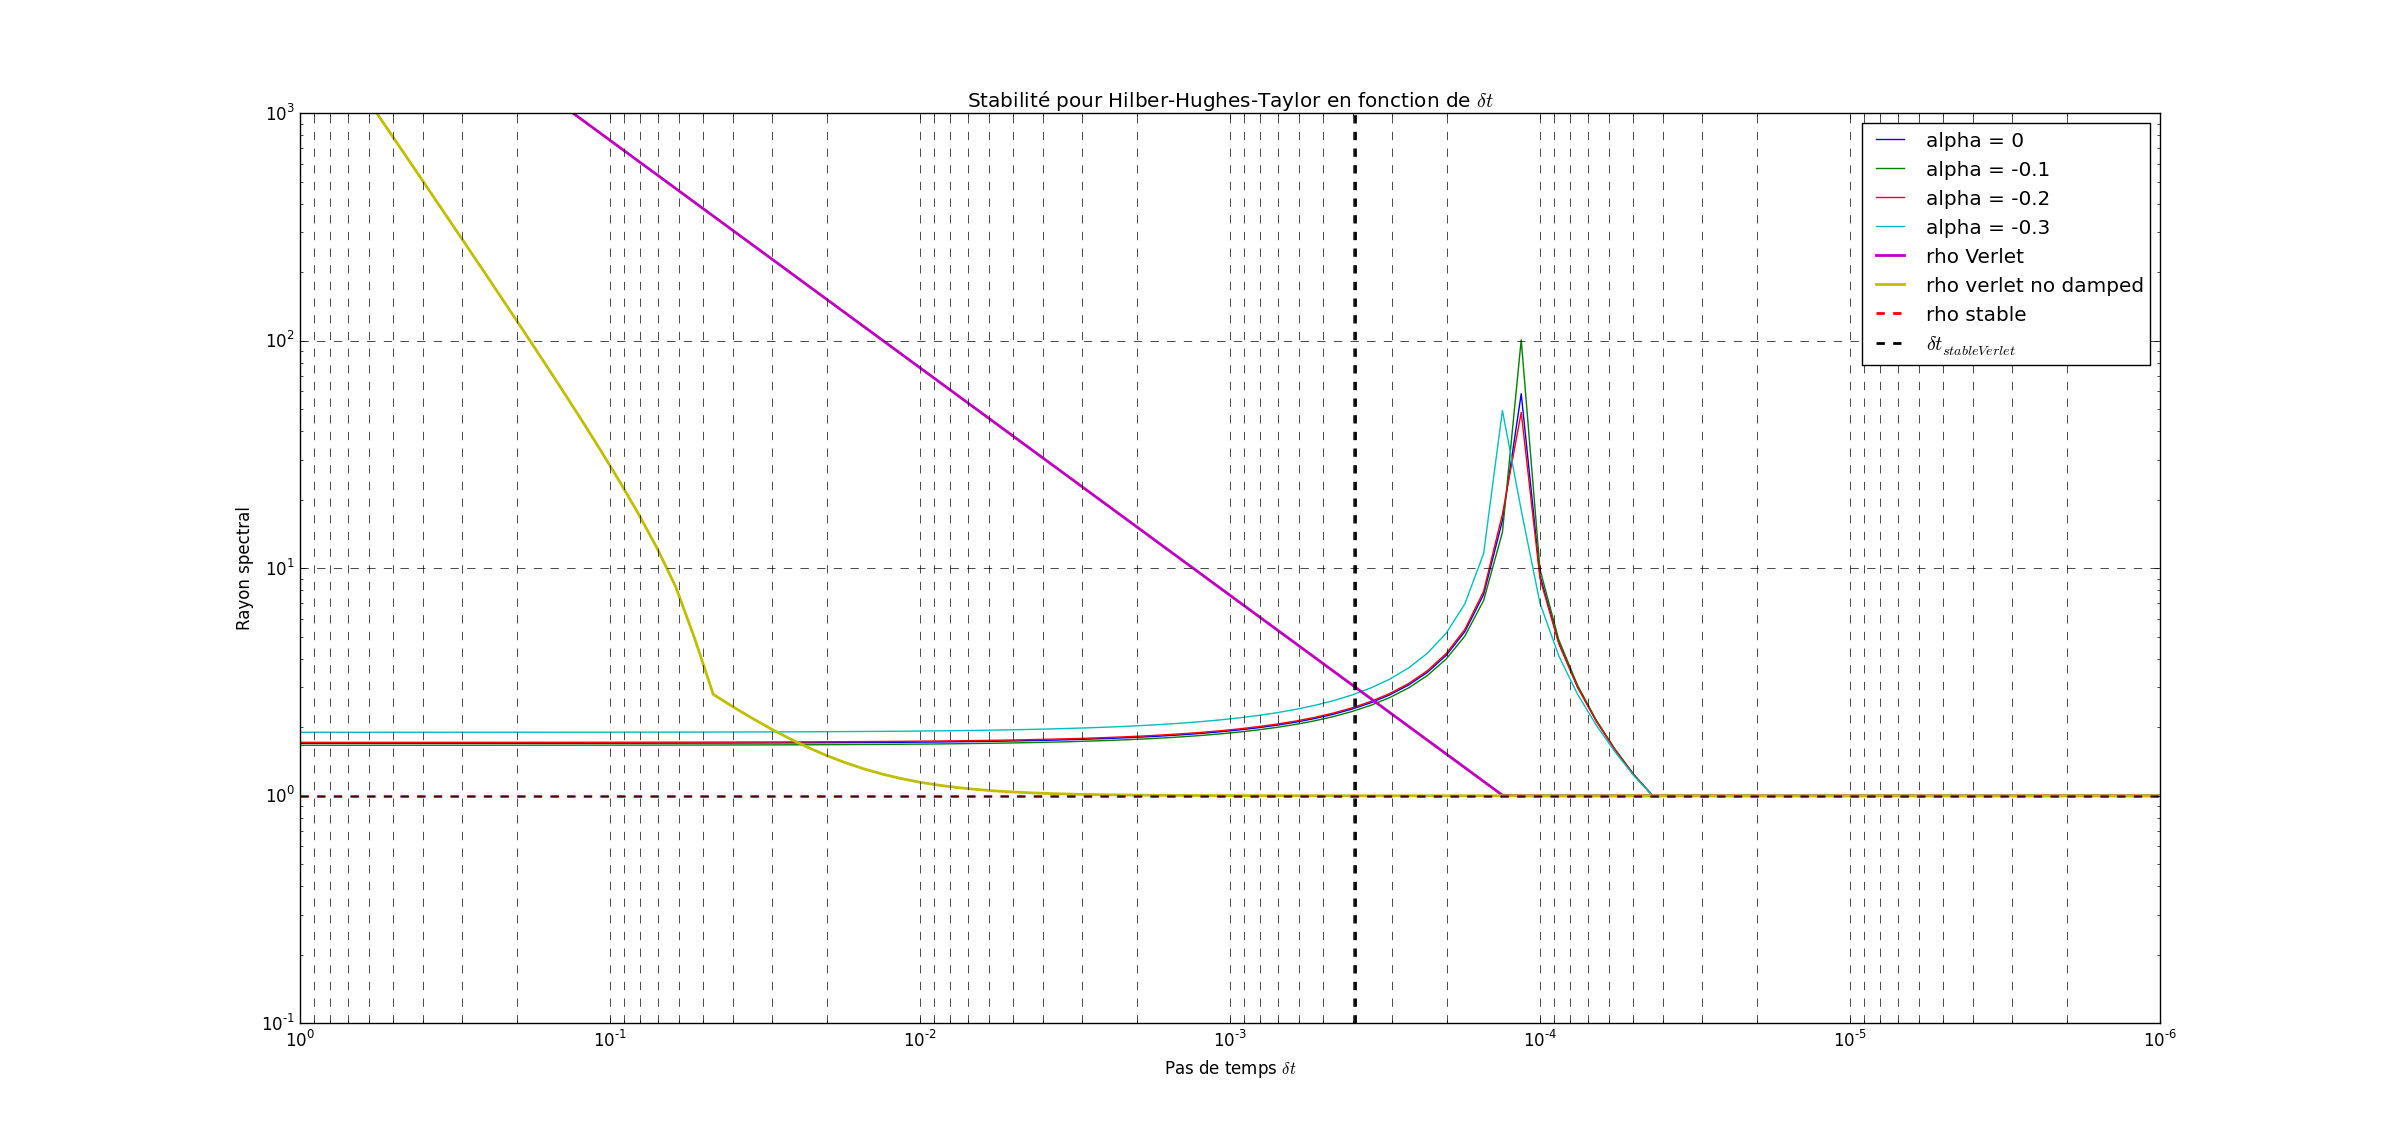
\includegraphics[width=1\linewidth]{figures/Part5/RhoVerlet.png}
	\label{RhoVerlet}
	\caption{Rayon spectral en fonction du pas de temps $\delta t$ appliqué au schéma de Verlet}
\end{figure}
\end{document}
